\documentclass[10pt,oneside]{report}

% Encoding and font packages
\usepackage[table]{xcolor}
\usepackage[utf8]{inputenc}
\usepackage[T1]{fontenc}
\usepackage{lmodern}
\usepackage{booktabs}
\usepackage{amsmath}
\usepackage{amsfonts}
\usepackage[nottoc]{tocbibind} % If you don't want the main TOC itself listed
\usepackage{setspace}
\onehalfspacing
\usepackage{hyperref}
\hypersetup{
    colorlinks=true,
    linkcolor=blue,
    filecolor=magenta,      
    urlcolor=cyan,
    citecolor=blue
}
\usepackage[numbers]{natbib}
\renewcommand{\citet}[1]{\citeauthor{#1}, \citeyear{#1}}

\usepackage[colorinlistoftodos,prependcaption,textsize=small]{todonotes}
\usepackage{adjustbox}
\usepackage{graphicx}
\graphicspath{ {./images/} }

\usepackage{anyfontsize}
\usepackage{lmodern}
% Dynamically scale font sizes (80% of original)
\let\oldsmall\small
\renewcommand{\small}{\fontsize{7}{8}\selectfont}
\let\oldnormalsize\normalsize
\renewcommand{\normalsize}{\fontsize{8}{10}\selectfont}
\let\oldlarge\large
\renewcommand{\large}{\fontsize{10}{12}\selectfont}
\let\oldLarge\Large
\renewcommand{\Large}{\fontsize{11.5}{13.8}\selectfont}
\let\oldLARGE\LARGE
\renewcommand{\LARGE}{\fontsize{13}{15.6}\selectfont}
\let\oldhuge\huge
\renewcommand{\huge}{\fontsize{16}{19.2}\selectfont}
\let\oldHuge\Huge
\renewcommand{\Huge}{\fontsize{20}{24}\selectfont}
\usepackage{subcaption}
\usepackage[font={normalsize},labelfont={bf}]{caption}

\DeclareCaptionType{equ}[][]
%\captionsetup[equ]{labelformat=empty}

\usepackage{color}
\usepackage{listings}
\usepackage{lipsum}


% Your provided environment setup:
\newcounter{nalg}[chapter] % defines algorithm counter for chapter-level
\renewcommand{\thenalg}{\thechapter .\arabic{nalg}} %defines appearance of the algorithm counter
\DeclareCaptionLabelFormat{algocaption}{Algorithm \thenalg} % defines a new caption label as Algorithm x.y
\lstnewenvironment{algorithm}[1][] %defines the algorithm listing environment
{
    \refstepcounter{nalg} %increments algorithm number
    \captionsetup{labelformat=algocaption,labelsep=colon} %defines the caption setup
    \lstset{ %this is the style
        mathescape=true, % Allows math mode with $...$
        frame=tB, % Top and bottom frame lines
        numbers=left,
        numberstyle=\tiny,
        basicstyle=\scriptsize\ttfamily, % Use typewriter font for code feel
        keywordstyle=\color{black}\bfseries, % Keywords bold (removed \em)
        keywords={input, output, return, function, in, if, else, foreach, for, while, begin, end, then, repeat, until, compute, select, assign, perform, update}, % Added more keywords
        commentstyle=\color{gray}\itshape, % Style for comments
        morecomment=[l]{\#}, % Define # as line comment start
        breaklines=true, % Allow line breaks
        breakatwhitespace=true,
        numbers=left,
        xleftmargin=.04\textwidth,
        #1 % this is to add specific settings to an usage of this environment
    }
}
{} % End of environment definition
% Begin document
\begin{document}

% -------------------------
% Title Page
% -------------------------
\begin{titlepage}
    \centering
    % Title (two lines)
    {\LARGE TODO TITLE\\\par}
    \vspace{2cm}
    % Subtitle/description
    {\large A report submitted to the University of Manchester for the degree of
    Bachelor of Science in the Faculty of Science and Engineering\par}
    \vspace{2cm}
    \vspace{1cm}

    {\large Author: Sai Putravu\par}
    {\large Student id: 10829976\par}
    {\large Supervisor: TODO\par}
    \vfill
    % Department
    % Date
    {\large 2025\par}
    \vspace{1cm}
    {\large School of Computer Science\par}
\end{titlepage}

% Roman page numbering for preliminary pages
\pagenumbering{roman}

% -------------------------
% Table of Contents
% -------------------------
\tableofcontents
\clearpage

% -------------------------
% List of Figures
% -------------------------
\listoffigures
\clearpage

% -------------------------
% List of Tables
% -------------------------
\listoftables
\clearpage


% -------------------------
% Abbreviations and Acronyms
% -------------------------
% \phantomsection
\addcontentsline{toc}{chapter}{Abbreviations and Acronyms}
\chapter*{Abbreviations and Acronyms}

\todo{Alphabetically sort this}
\begin{table}[ht]
    \centering
    \begin{tabular}{ll}

        \textbf{AE} & Auto-encoding. \\
        \textbf{AR} & Auto-regressive. \\
        \textbf{BERT} & Bidirectional Encoder Representation from Transformers. \\
        \textbf{CBM} & Condition-based maintenance policy. \\
        \textbf{CLI} & Command Line Interface. \\
        \textbf{CNN} & Convolutional Neural Network. \\
        \textbf{CPU} & Central Processing Unit. \\
        \textbf{CUDA} & Compute Unified Device Architecture. \\
        \textbf{DBSCAN} & Density-Based Spatial Clustering of Application with Noise. \\
        \textbf{DL} & Deep Learning. \\
        \textbf{ELMo} & Embeddings from Language Models. \\
        \textbf{EPB1} & Extracted proton beam line 1. \\
        \textbf{EPB2} & Extracted proton beam line 2. \\
        \textbf{FAP} & Fault Analysis Pathway. \\
        \textbf{FLD} & First-line diagnosis system. \\
        \textbf{GPT} & Generative Pre-trained Transformer. \\
        \textbf{GPU} & Graphics Processing Unit. \\
        \textbf{HDBSCAN} & Hierarchical Density-Based Spatial Clustering of Application with Noise. \\
        \textbf{HDD} & Hard-Disk Drive. \\
        \textbf{HEDS} & High energy drift space. \\
        \textbf{IoT} & Internet of Things. \\
        \textbf{LEBT} & Low energy beam transport line. \\
        \textbf{LINAC} & Linear Accelerator. \\
        \textbf{LSA} & Latent Semantic Analysis. \\
        \textbf{MCR} & Main Control Room. \\
        \textbf{ML} & Machine Learning. \\
        \textbf{MST} & Minimum Spanning Tree \\
        \textbf{MRL} & Matryoshka Representation Learning. \\
        \textbf{MTEB} & Massive Text Embedding Benchmark. \\
        \textbf{NLP} & Natural Language Processing. \\
        \textbf{Operalog} & The ISIS Operational Log. \\
        \textbf{PAM} & Partitioning Around Medoids. \\
        \textbf{PCA} & Principle Component Analysis. \\
        \textbf{PdM} & Predictive maintenance policy. \\
        \textbf{PLM} & Pre-trained Language Model. \\
        \textbf{PvM} & Preventative maintenance policy. \\
        \textbf{R2F} & Run-to-failure maintenance policy. \\
        \textbf{RAM} & Random Access Memory. \\
        \textbf{RFQ} & Radio-frequency quadrupole. \\
        \textbf{RF} & Random Forest. \\
        \textbf{RoPE} & Rotary Positional Embeddings. \\
        \textbf{SAFE} & Supervised Aggregative Feature Extraction. \\
        \textbf{SMART} & Self-monitoring and reporting technology. \\
        \textbf{STFC} & Science and Technology Facilities Council. \\
        \textbf{SVD} & Singular Value Decomposition. \\
        \textbf{SVM} & Support Vector Machine. \\
        \textbf{TS-1} & Target Station 1. \\
        \textbf{TS-2} & Target Station 2. \\
        \textbf{t-SNE} & t-distributed Stochastic Neighbour Embedding. \\
        \textbf{UKRI} & United Kingdom Research and Innovation. \\
        \textbf{UMAP} & Uniform Manifold Approximation and Projection. \\
        \textbf{VRAM} & Video Random Access Memory. \\

    \end{tabular}
\end{table}

\clearpage

% Switch to Arabic numbering after preliminary pages
\pagenumbering{arabic}

% -------------------------
% Chapters
% -------------------------
\chapter*{Abstract}
\todo[inline]{TODO}


\chapter{Introduction}

This project concerns the use of statistical and machine learning models to augment the predictive maintenance process at the STFC Rutherford Appleton Laboratory's ISIS Neutron and Muon research facility. The ISIS Neutron and Muon facility is a research centre for physical and life sciences, owned and operated by the STFC, a council that forms the UK Research and Innovation. In order to produce beams of neutrons and muons, allowing scientists to study materials at the atomic level, large and complex structures and machinery are required. The facility has a wealth of instrumentation taking multitudes of measurements to ensure that proper maintenance is completed in a timely manner. \\

\todo[inline] {Finish this off, also mention this is one of two parts. And this aims to focus on the Operalog, a rich textual record of real-world failures of the of the ISIS facility.

Also, mention that this is a very open-ended research project and what we should be judged on? i.e. progressing the space of auto-categorisation of industrial operational logs.

Also mention there is no "industry standard" for this to compare it to. 
}

\textbf{ }
\todo[inline,caption={}]{
Introduce the sections of the paper.
\begin{itemize}
    \item Refine this after coming back
    \item Section 2,
    \item Section 3, 
    \item ...
\end{itemize}
}


\section{Motivation}
Motivate the research project.


\todo[inline,caption={}]{
The things in this section will include
\begin{itemize}
    \item Introduce the problem: Auto-categorisation and label inference
    \item Highlight the research aims. This should highlight the vastly open nature of the project and then hone in on the particular issue I am tackling. (i.e. to progress the state of PdM ...)
    \item Identify the data input, expected output, data shape and explain why this motivates the project
\end{itemize}
}


\section{Overview of the ISIS Research Facility}\label{sec:isisbg}

The STFC Rutherford Appleton Laboratory's ISIS Neutron and Muon research facility is a research centre for physical and life sciences. It is owned and operated by the STFC, a council within the United Kingdom Research and Innovation (UKRI). The UKRI is a public body of the United Kingdom's Government that directs funding for research and innovation through the science budget of the Department for Science, Innovation and Technology. ISIS was designed in the 1970s and early 1980s, with the core of the design being a strong-focusing machine with six radio frequency accelerating cavities to provide an average beam current of $200\mu A$ \cite{thomason2019isis}. According to (\citet{thomason2019isis}), with the introduction of ISIS and other neutron sources, rapid development of neutron instrumentation was stimulated. Over the years, the facility has been augmented with numerous components and instruments, such as the second target station. The current schematic representation of the facility can be seen in Figure~\ref{fig:isis}.

\begin{figure}[htbp]
    \centering
    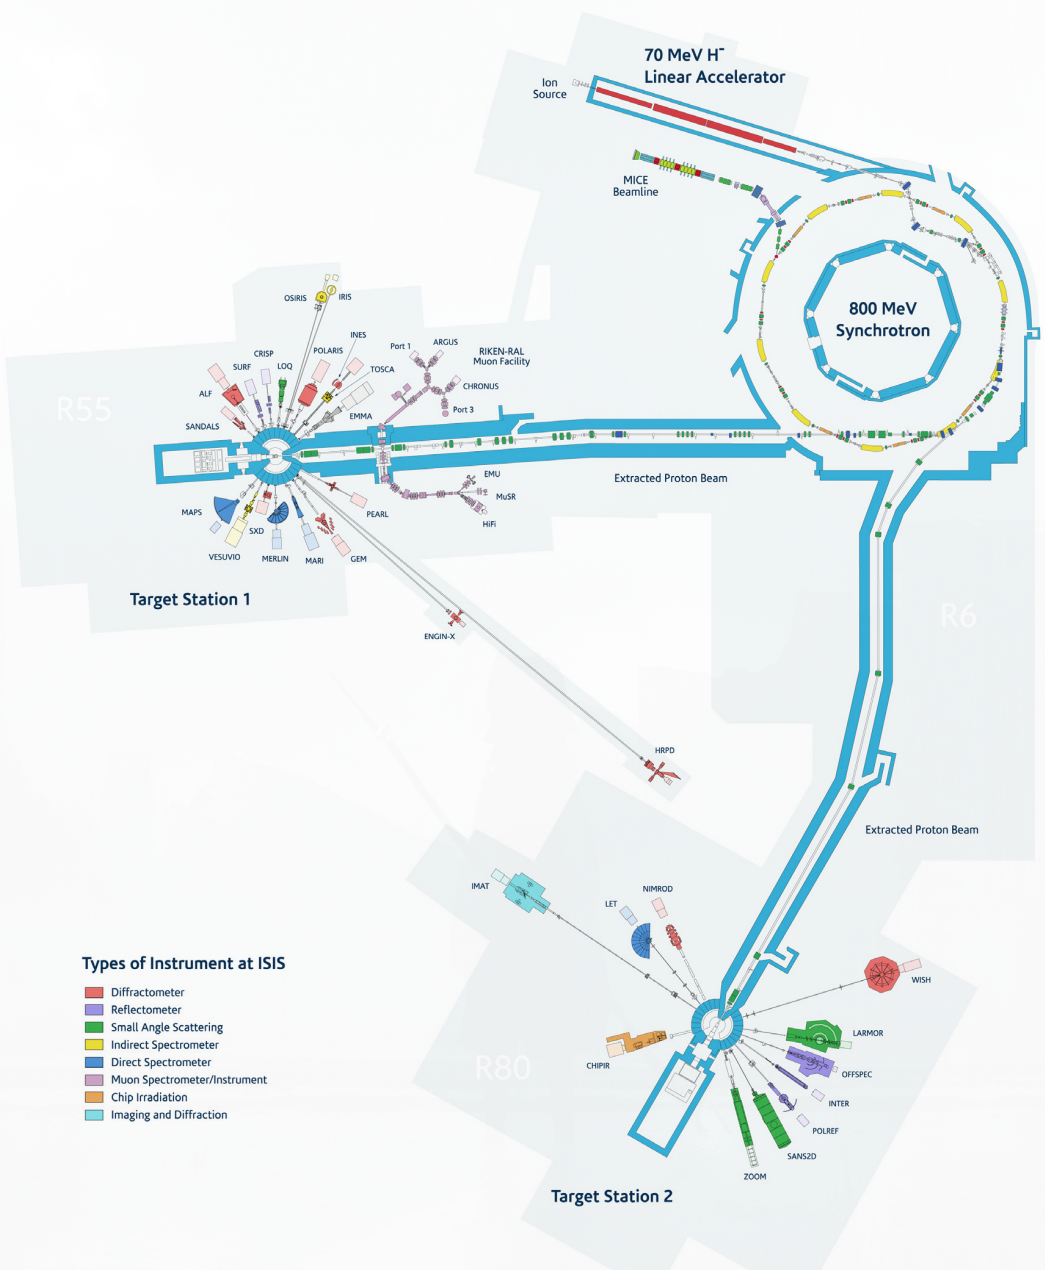
\includegraphics[width=0.95\textwidth]{ISIS.png}
    \caption{The schematic representation of the physical layout of ISIS. The light grey areas are footprints of the buildings. Source: (\citet{thomason2019isis}).}\label{fig:isis}
\end{figure}

\subsection{The end-to-end production of neutrons and muons}
\begin{figure}[htbp]
    \centering
    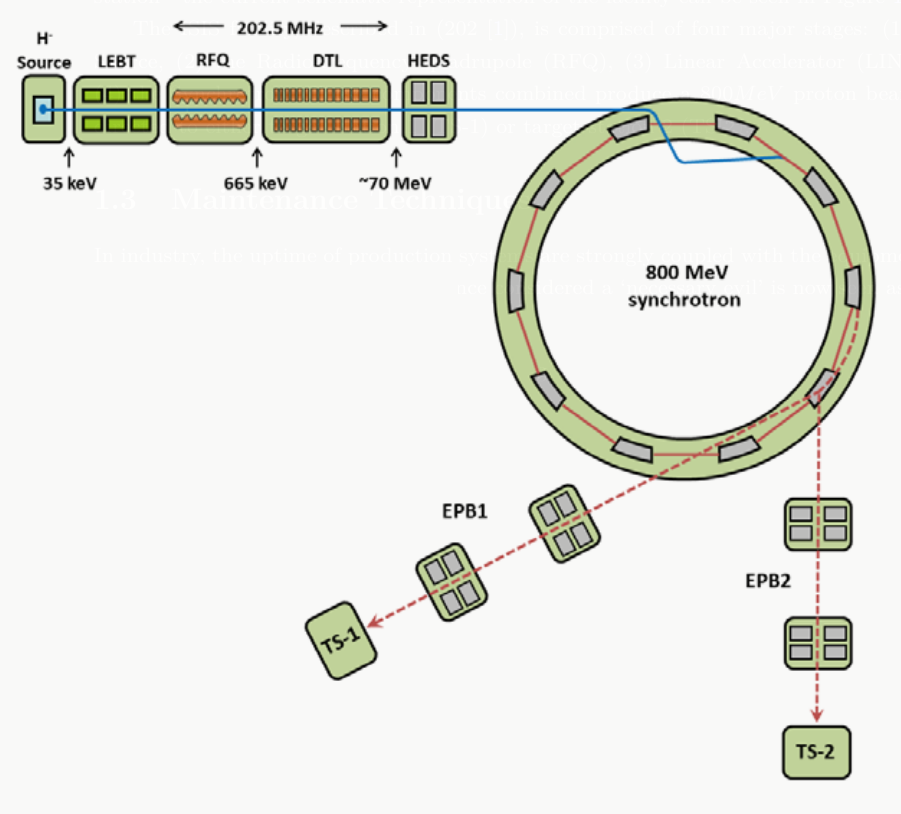
\includegraphics[width=0.6\textwidth]{ISIS2.png}
    \caption{ISIS ion source and chain of accelerators, with $H^-$ ions in blue and protons in red. Not to scale. Source: (\citet{2021practicalguide}).}\label{fig:isis2}
\end{figure}

The ISIS facility, described in A Practical Guide to the ISIS Neutron and Muon Source (\citet{2021practicalguide}), is comprised of four major stages: (1) the ion source, (2) the radio-frequency quadrupole (RFQ), (3) linear accelerator (LINAC) and (4) the synchrotron. These components combine to produce a 800 MeV proton beam that is directed to either target station 1 (TS-1) or target station 2 (TS-2). Starting with $H^-$ ions (protons with two orbiting electrons), the path taken through the four stages is shown in Figure~\ref{fig:isis2}. Throughout the entire $H^-$ or proton acceleration process, the beam must be kept under tight vacuum and, to do so, many tens of vacuum pumps are maintaining the vacuum between $10^{-8}$ and $10^{-9}$ of atmospheric pressure. Maintaining this vacuum integrity is a constant operational challenge as leaks may disrupt the beam and potentially damage sensitive components, necessitating numerous pumps and continuous monitoring system \cite{2021practicalguide}. The rest of this section explains the various stages in a more detail with the purpose of highlighting the complex infrastructure in place and critical control required for the reliable operation of the facility.

The first stage of the ISIS machine is the ion source, which generates the negative hydrogen ($H^-$) ions, which are then accelerated through the RFQ and LINAC. This ion source is a pulsed source that ionises hydrogen gas via an electric discharge between an internal anode and cathode \cite{2021practicalguide}. As detailed in the guide, around 20ml of hydrogen gas per minute is continuously delivered to the ion source from a hydrogen gas bottle. Once the $H^-$ ions emerge from the ion source, they have an energy of 35 keV and are presented to the RFQ via the Low Energy Beam Transport line (LEBT). The LEBT prevents the low-energy $H^-$ beam from increasing in size (due to the mutual repulsion of the ions) and also incorporates a beam stop. This is essentially a remotely removable sheet of metal that physically blocks the beam. Precise control and monitoring of the beam intensity are required here since inconsistencies originating from the ion source affect the overall performance of the machine. This is because these issues can propagate and amplify through the subsequent stages. Additionally, the failure of the source itself, for example due to component wear, requires immediate intervention and is a common maintenance task \cite{2021practicalguide}.

Following the ion source and LEBT, the $H^-$ beam enters the RFQ. This section of the machine utilises high-intensity radio frequency electric fields that contain (focus), group (bunch) and begin accelerating the particles in this beam up to an energy of 665 keV. A key function of the RFQ is to isolate downstream accelerators from variations originating in the ion source, thereby improving beam stability in the LINAC, synchrotron and target stations \cite{2021practicalguide}. However, the stability of the RFQ's own high-intensity beam is a primary concern as, again, fluctuations can lead to poorly formed bunches.

The subsequent stage is the LINAC, which increases the beam energy from 665 keV to 70 MeV. This acceleration is achieved via high-intensity radio-frequency fields arranged in structures that possess a very high Q factor \cite{michael2006electronic} (around 50,000). This means their geometry must be exceptionally stable. Therefore the precise temperature regulation of the cooling water tank is critical in ensuring it is significantly under $1^\circ C$ so that the effects of thermal expansion and contraction are countered \cite{2021practicalguide}. Furthermore, maintaining a high vacuum is critical throughout the LINAC. Failure to do so can lead to premature stripping of loosely bound electrons in the $H^-$ ions, consequently leading to an increase in radioactivity and particle loss (i.e. beam loss). To detect and warn about such cases, beam loss monitors are installed throughout the LINAC, which provide an indication whenever there is an excessive loss in particles. \cite{2021practicalguide}.

Once the $H^-$ particles leave the LINAC, they then pass through a beam transport line - the High Energy Drift Space (HEDS). The function of this is to mainly reduce the particles spreading and focus the beam to the synchrotron. To accumulate the high intensity beam in the synchrotron, ISIS employs charge-exchange injection. This technique allows incoming $H^-$ beam from the LINAC to be `layered' into the synchrotron's circumference over many turns. As the $H^-$ ions enter the synchrotron ring, they pass through a thin foil which strips away their two electrons, converting them to protons. The charge-exchange injection process is specifically chosen as it is the most efficient way of taking and wrapping a long string of particles around the circumference of a synchrotron \cite{2021practicalguide, ankenbrandt1980h}. The integrity of this thin foil is vital for efficient injection and represents a consumable component requiring periodic replacement, which is a scheduled maintenance activity. Damage to the foil will lead directly to beam loss and reduced performance.

The 70 MeV beam is then injected into the synchrotron, which is the primary accelerator ring at ISIS. This ring boosts the (now proton) beam energy to 800 MeV. For an idea of scale, the machine has a circumference of around 163m (corresponding to a radius of approximately 26m). It features a repeating structure of ten `superperiods'. Each superperoid uses dipole magnets to bend the proton path by $36^\circ$ and quadrupole magnets to maintain beam focus \cite{2021practicalguide}. The protons gain energy over just under 8000 revolutions, as each turn gives a proton 0.1 MeV. Achieving this final energy requires extreme precision over each and every revolution. While the protons gain energy, the magnetic fields and accelerating radio-frequency voltages must also very precisely be increased in synchronism. Any deviations can cause the beam to oscillate and strike the vacuum vessel walls which results in particle loss and potential component damage. Therefore, continuous precise monitoring of beam position, magnet currents and more via a network of sensors is imperative for controlling the beam orbit and ensuring successful acceleration \cite{2021practicalguide}. The initially continuous ring of injected protons is gathered into two distinct bunches, a little more than $0.1\mu s$ apart, using a low-level radio-frequency voltage before the main acceleration begins \cite{2021practicalguide}.

Once accelerated, in order to direct the proton bunches towards a pre-selected target station (TS-1 or TS-2) three kicker magnets are used which deflect the bunches upwards. These bunches are then bent into the respective extracted proton beam lines (EPB1 or EPB2). These lines use further magnets for steering. Safe transport relies on accurate magnet performance as mis-steering could direct the high-energy beam into the pipe walls. Additionally, as a safety precaution, both lines are heavily shielded in thick steel and concrete and beam loss monitors are installed along their length to detect any errant particles and provide crucial, real-time feedback to operators \cite{2021practicalguide}.

The primary purpose of the ISIS facility culminates at the target stations. The high-energy proton beam collides with a dense, high atomic number target (tantalum-clad tungsten at ISIS), designed to produce a large number of neutrons via spallation, within a compact region of space \cite{2021practicalguide}. These energetic neutrons are then slowed down (moderated) by surrounding materials (liquid nitrogen, liquid hydrogen and water at ISIS) and reflected back towards instruments by a beryllium reflector \cite{sharma2001nuclear, 2021practicalguide}. Additionally, ISIS produces muons for experiments by inserting a thin (roughly 1cm thick) graphite target into the proton beam around 20m away from the TS-1 neutron target. Collision in this target generates pions, which subsequently decay into muons \cite{2021practicalguide}.
This entire system needs extremely careful control and monitoring capabilities, as failure due to overheating or material damage is a major operational concern which requires careful management and represents a major maintenance undertaking. Precise monitoring is required of metrics such as incoming beam profile, target temperature, cryogenic temperatures. \\

\noindent This detailed description sourced from the guide highlights some key takeaways. There are an incredible number of points of failure in the facility due to the highly precise and radioactive nature of the task. The ISIS team has taken many precautions such as fault detection mechanisms (i.e. the beam loss monitors) and breakdown counter-measures (i.e. the thick layer of steel and concrete in the EPB1 and EPB2 lines). However, the inherent complexity and harsh operating environment (radiation, high-power) necessitate both robust preventative maintenance schedules and sophisticated diagnostic capabilities that address the component degradation and failures that will inevitably arise. 

\subsection{Maintenance at ISIS} 
As detailed in the 33-year historical account of the ISIS facility (\citet{thomason2019isis}), the ISIS operations occur in cycles, periods of roughly 30-50 days where the machine runs constantly without breaks. Gaps between cycles typically range from 1 week to 3 months. In addition, typically every four years, shutdowns scheduled for 6-9 months occur for major maintenance and upgrade work. On the ground, day-to-day operations are run from the Main Control Room (MCR) by the ISIS crew which consists of 6 shift teams of the following roles: (1) duty officer, (2) assistant duty officer and (3) duty technician. \todo{Add the graph, if you can ever figure out the operating cycles before 2016.} The expertise and rapid response capabilities of these trained operational crews are vital for both routine operation and initial fault response.
Minimising this downtime is crucial for several reasons inherent to operating a large-scale user facility like ISIS \cite{thomason2019isis}. Primarily, unscheduled downtime directly impacts the international researchers allocated beam time, potentially jeopardising experiments planned months or years in advance and wasting valuable research opportunities. Furthermore, interruptions disrupt the tightly packed operational schedule, reduce the overall scientific output, and incur significant operational costs without delivering the facility's core research product \cite{thomason2019isis}. Therefore, understanding the factors that contribute to downtime and implementing strategies to mitigate it are paramount.
Many factors affect downtime such as having a robust plan, the day-to-day operators' knowledge of the system and adequate inventories of spares \cite{thomason2019isis}. Figure~\ref{fig:isisDowntime} shows the ratio of downtime to active machine operation since 2016, indicating this machine has been down for maintenance over half the time since 2016. In other words, over half the time, the machine is not active and is undergoing maintenance. This highlights the trade-off between maximising operational availability and minimizing failures through planned maintenance. The major maintenance strategies and their trade-offs are further explored in Section~\ref{sec:maintenanceTechniques}.

To help reduce downtime, over the last few years, a first-line diagnosis (FLD) system was introduced, presented in (\citet{fld2017}). The FLD system helps reduce downtime by providing expert guidance on fault diagnosis and resolution, which has been shown to improve the dissemination of knowledge from experts to operations. The FLD utilises Fault Analysis Pathways (FAPs), which provide structural links between ISIS subsystems. This allows users of the system to access granular subsystems' local documentation minimising file hunting and saving time and effort. An example FAP can be seen in Figure~\ref{fig:fap}.

\begin{figure}[htbp]
    \centering
    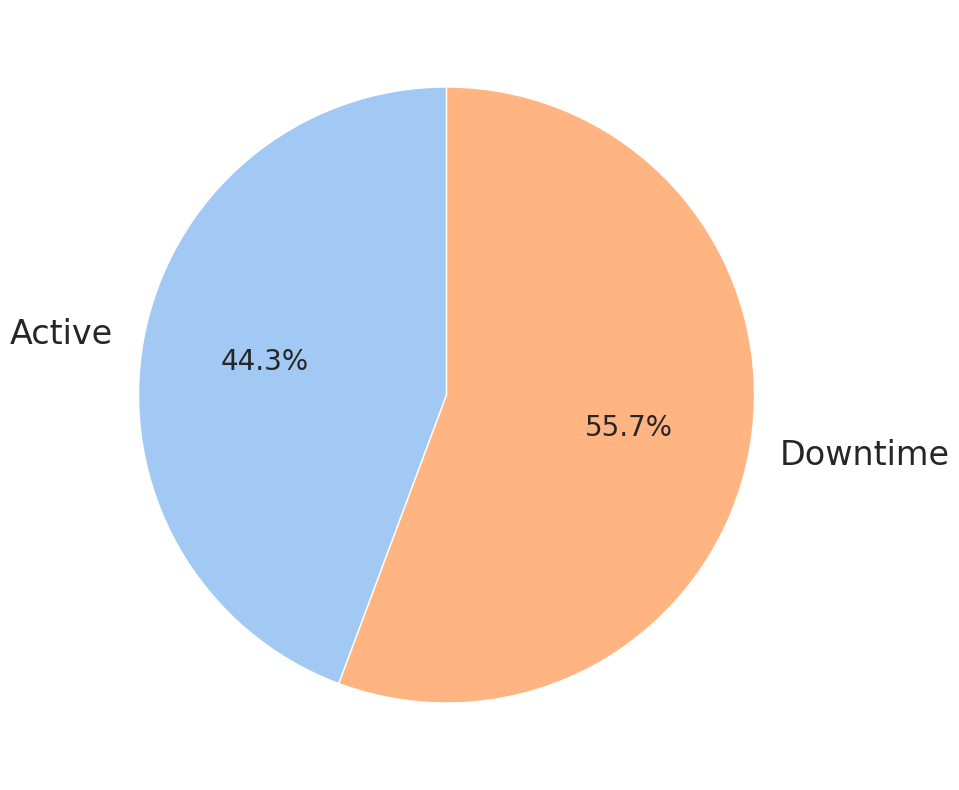
\includegraphics[width=0.5\textwidth]{isisDowntime.png}
    \caption{A visualisation of the machine downtime as opposed to time operating, according to the ISIS operational cycle. Data source: (\citet{isisbeamoperations2024})}\label{fig:isisDowntime}
\end{figure}
\begin{figure}[htbp]
    \centering
    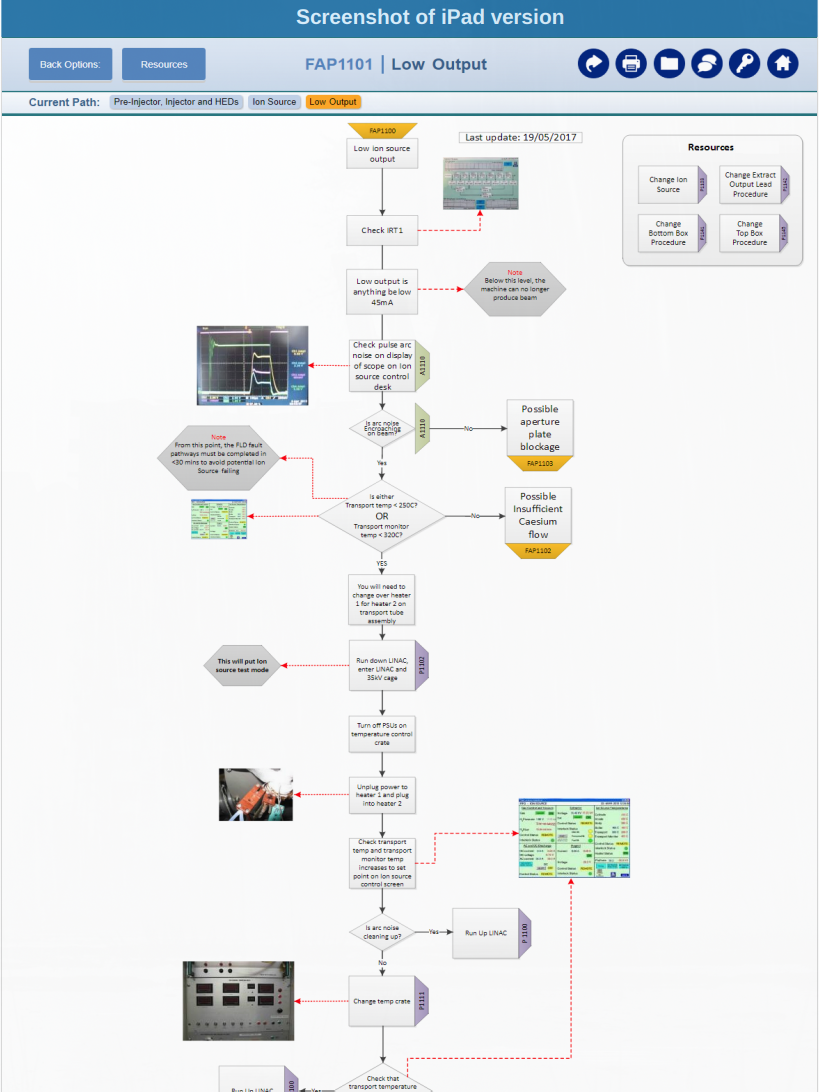
\includegraphics[width=0.95\textwidth]{fap.png}
    \caption{Example FAP1101, screenshotted from an iPAD version of FLD version 2.2, which shows the FAP for pre-injector, injector and High Energy Drift Space. Source: (\citet{fld2017})}\label{fig:fap}
\end{figure}


% \textbf{}\\
% \todo[inline,caption={}]{
% Introduce the research topic. 
% The things in this section will include
% \begin{itemize}
%     \item Talk about the ISIS research facility - DONE
%     \item Talk about the Operational Cycle for ISIS - SORT OF DONE (graph too)
%     \item Talk about the ISIS Crew and importance of having trained staff on premises. - SORT OF
%     \item Talk about the Lost time and why it is important to minimise this for the ISIS research facility. - SORT OF
%     \item Describe the first-line diagnosis system (FLD) and FAPs. - DONE
%     \item Talk about the Datasets, operalog (MOVED)
% \end{itemize}
% }


\section{Maintenance Techniques}\label{sec:maintenanceTechniques}
In industry, the uptime of production systems is strongly coupled with the equipment maintenance. So much so that what was once considered a `necessary evil' is now seen as a `profit contributor' to be able to maintain a competitive edge \cite{waeyenbergh2002framework, faccio2014industrial}. For facilities aiming to provide systems for research, maintenance impacts the downtime and cost of running. As a result, both to minimise unexpected downtime and provide a competitive edge, many industrial applications collect vast quantities of data during the entire life cycle of the system. This large amount of data may include information about processes, events and alarms \cite{carvalho2019systematic} which occur along the industrial production line, collected by different equipment. The equipment may be located in different locations in the sub-components of the larger system or even different sub-components themselves. 

% \todo{talk about maintenance itself in a lot more depth}

In the literature, various terms and categories of maintenance arise each with differing strategies \cite{susto2012predictive, mobley2002introduction, susto2016dealing}. Thus, while there exists some disagreement in nomenclature, we consider the four categories presented in (\citet{susto2012predictive}). The four maintenance policy categories are as follows, noting that each policy has, uniquely, their own benefits and drawbacks:

\begin{enumerate}
    \item{Run-to-failure (R2F) maintenance: Continual usage of the system until failure. Restoration is performed at the point of noticing failure condition. This is the simplest approach and typically the most costly method as it reduces the facility's availability and requires a complete replacement of parts.} 
    \item{Preventative maintenance (PvM): Otherwise referred to as scheduled maintenance, performing maintenance at regular intervals to increase longevity of the component or in anticipation of the end of expected life of the component. While this typically prevents many errors, it wastes maintenance cycles when systems are perfectly healthy. Hence, causing unnecessary downtime and cost.}
    \item{Condition-based maintenance (CBM): Taking the action to perform maintenance on equipment through monitoring various health characteristics and metrics of the components of the system. This approach requires continuous monitoring and, thus, allows for close to instant response on maintenance only when required. However, a drawback of this policy is that one cannot plan maintenances in advance.}
    \item{Predictive maintenance (PdM): Otherwise referred to as statistical-based maintenance, only performs maintenance actions when determined necessary. Prediction tools are utilised to implement forward-planning and scheduling systems, using statistical inference methods. However, if these statistical inferences are not accurate, the whole system suffers which inevitably leads to additional downtime and costs.}
\end{enumerate}
It should be noted that several sources conflate CBM and PdM \cite{mobley2002introduction}. As in (\citet{susto2012predictive}), where they are given as separate categories, we follow suit. \\ 

The PdM strategy stands out in the four categories presented as, given a statistical inference model that is able to detect faults accurately, this policy optimises the trade-off between improving equipment condition, reduce failure rates for equipment and minimising maintenance costs \cite{carvalho2019systematic}. This technique enables one to apply foresight for pre-emptive scheduling of large-scale maintenance. As pointed out in Section~\ref{sec:isisbg}, the ISIS facility aims to strike a balance between PvM, CBM and PdM through periods of large-scaled scheduled maintenance and collection of high quantities of metrics. This balance is achieved through the careful coordination between cycle scheduling, day-to-day crew-based monitoring and the FLD \cite{thomason2019isis}.

In industry, many maintenance strategies prefer using PdM whilst experimenting with a variety of statistical inference and artificial intelligence modelling approaches \cite{mobley2002introduction, jezzini2013effects}. Some examples from \cite{carvalho2019systematic} are listed in Table~\ref{tab:pdmPaperTable} which highlights the trend in the industry towards more accurate, ML-based approaches.

\rowcolors{2}{gray!10}{white}
\begin{table}[htbp]
    \fontsize{8}{12}\selectfont
    \centering
    \caption{Examples of applications of PdM for industrial maintenance strategies.}
    \label{tab:pdmPaperTable}
    \begin{adjustbox}{max width=\textwidth}
    \begin{tabular}{p{1.5cm} p{8.5cm} p{3cm}}
        \toprule
        \textbf{Type} & \textbf{Description} & \textbf{Reference} \\
        \midrule
        Statistical & Application of SAFE to deal with PdM problems characterised by time-series data. The approach is tested on a real-life dataset of the semiconductor ion implantation process. & (\citet{susto2016dealing})\\
        ML & Application of SVM classification for fault prediction of rail networks, with discussion on using the model in optimising trade-offs related to maintenance schedule and costs. & (\citet{li2014improving})\\
        ML & Audio analysis on IoT devices, enabling acoustic event recognition for machine diagnosis. This paper describes designing an end-to-end system, utilising CNN-based classification. & (\citet{pan2017cognitive})  \\
        ML & Utilisation of RF decision trees trained on SMART data to predict reliability of HDD in real-time. & (\citet{su2018real}) \\
        \bottomrule
    \end{tabular}
    \end{adjustbox}
\end{table}



\chapter{Natural Language Processing Background}

This chapter delves into the technical background required for the methodology proposed in Chapter \ref{chap:Methodology}. Firstly, we discuss various measures of text similarity in Section \ref{sec:sentenceSimilarity}, which motivates text embeddings and categorises similarity measures into different generations. Section \ref{sec:sentenceEmbedding} introduces both third‑generation model BERT \cite{devlin2019bert} and the more recent fourth‑generation universal‐embedding architecture XLNet \cite{yang2019xlnet}. We specifically discuss the technical details of the BERT model and further iterations on it, then detail one improvement over BERT (XLNet) and outline the design principles that underpin contemporary fourth‑generation models. Afterwards, we cover two methods of dimensionality reduction,  PCA \cite{pearson1901liii,hotelling1933analysis} and UMAP \cite{mcinnes2018umap}, motivated by the need to visualise samples from the high‑dimensional embedding spaces of the aforementioned models, in Section \ref{sec:dimred}. Finally, we present three clustering algorithms—one partitioning‑based (k‑Medoids \todo{Fill this}\cite{}) and two density‑based (DBSCAN \cite{ester1996density} and HDBSCAN \cite{campello2013density})—together with four clustering‑evaluation metrics: (1) Inertia \todo{find the reference for this}\cite{}, (2) Silhouette \cite{rousseeuw1987silhouettes}, (3) Davies–Bouldin Index \cite{davies1979cluster}, and (4) Calinski–Harabasz Index \cite{calinski1974dendrite}. \todo{maybe talk about optuna, if we use it.} \todo{double check all citations here are not empty}\


\todo[inline,caption={}]{
Describe the various technical factors required before attempting to understand the methodology.
The things in this section will include
\begin{itemize}
    \item Discuss sentence embedding, similarity measures: BERT, RoBERTA, MPNet, XLNet, NOMIC.
    \item Dimensional reduction techniques and need for them (UMAP, PCA, t-SNE).
    \item Clustering methods: kmedoids, DBSCAN, DBSCAN*/HDBCAN
    \item Clustering evaluation methods: todo I don't remember these off the top of my head 
    \item Maybe briefly touch on Optuna?
\end{itemize}
}

\section{Sentence Similarity}\label{sec:sentenceSimilarity}
Sentence similarity, otherwise referred to as document similarity, is the (NLP) task of computing the quantification of the similarities between two sentences, documents or texts. This task is motivated by the increasingly large amount of digitisation of human languages (and data, in general), calling for the need to understand similarity between various texts \cite{raju2022sentence}. Examples of the use-cases of sentence similarity include: detection of academic malpractice via plagiarism \cite{lukashenko2007computer, baba2017plagiarism}, and text summarisation \cite {aliguliyev2009new, kumar2020semantic, jo2017k}. According to \cite{raju2022sentence}, there are two main types of sentence similarities: (1) lexical similarity and (2) semantic similarity. The former is a computation of the equality between the lexicon of two sentences (i.e. a purely syntactical view). This contrasts with semantic similarity, which compares meaning. Further, the type we focus on, semantic similarity can be split into three types: 

\begin{itemize}
    \item String-based similarity: Measures similarity directly between two strings, accounting for string sequences and character composition. These can be fine-grained, i.e. character-based; coarse-grained, i.e. term-based; or a hybrid mixture of both \cite{yu2016string}.
    \item Knowledge-based similarity: Measures the degree to which two sentences are related, utilising semantic networks (i.e. knowledge graphs). Examples of Knowledge-based similarity approaches include WordNet \cite{budanitsky2001semantic}, the most popular type of approach.
    \item Corpus-based similarity: Premised on a provided corpus, a large database of text to derive inferences from. Methods of this type require the development statistical or DL models that train on the provided corpus and estimate the similarity between two sentence-pair inputs. Popular examples include traditional statistical models, such as LSA \cite{landauer1998introduction} and SVD \cite{steinberger2005text} as well as word embedding models (utilising ML), such as Word2Vec \cite{bojanowski2017enriching}, GloVe \cite{pennington2014glove} and fastText \cite{mikolov2013efficient}.
\end{itemize}

Most of the models mentioned above require some numerical representation of the text to be able to apply mathematical procedures for similarity calculation. Computing this representation involves converting unstructured textual data into one or more vectors. Typically, this process includes (1) general natural language pre-processing steps such as stop-word removal, case normalisation, parts-of-speech tagging, lemmatisation, and tokenisation \cite{tabassum2020survey}; and (2) applying an embedding model, either to a single token (word embedding) or to a sequence of tokens (sentence embedding). Step (1) can be seen as a feature extraction step applied on the unstructured textual data, where feature extraction is the process of extracting the most useful components of the data \cite{sammons2016edison}. For example, part-of-speech tagging can be seen as introducing non-trivial features to some token through extracting the surrounding context. 

This representation is known as an embedding, with the span of the possible vectors referred to as the embedding space. The dimension of the span is termed the embedding dimension. This is an important concept because the characteristics of the embedding space influence the model's ability to capture syntactic and semantic meaning in text, as the embedding space itself encodes this information. This can be seen in the Word2Vec model, described in (\citet{bojanowski2017enriching}), which shows different embedding dimensions produce different results. Another conclusion that can be drawn from this paper is that, if embedding space is not constructed to maximise the meaning of texts, the accuracy of model predictions tends to deteriorate. 

Therefore, the problem of sentence similarity can be directly mapped from the problem of sentence embedding (otherwise referred to as text embedding), where text embedding is the (NLP) task of learning a high-dimensional embedding space representation. Various aspects of text embedding are more thoroughly covered in Section~\ref{sec:sentenceEmbedding}. However, with the advent of the transformer architecture \cite{vaswani2017attention} and rise of the large language models, text embedding has been increasingly solved using DL models with high parameter counts \cite{cao2024recent} and considering extremely large token sequences. Nowadays, word embedding models are considered obsolete with (\citet{cao2024recent}) only considering these models second-generation. Further, the paper states newer generations fall into the following categories:
\begin{itemize}
    \item Third-generation: contextualised embeddings. These models dynamically account for contexts, encoding them into the embedding space. Examples of models include ELMo \cite{sarzynska2021detecting}, GPT \cite{radford2018improving} and BERT \cite{devlin2019bert}. As these models are trained to both understand some embedding space and generate natural language text, they are canonically referred to as language models.
    \item Fourth-generation: universal text embeddings. The generation which is currently state-of-the-art, with the aim of developing a unified model which is able to address multiple downstream tasks. Examples of models in this generation, making progress towards unification include Gecko \cite{lee2024gecko}, Multilingual e5 text embeddings \cite{wang2024multilingual}, Nomic \cite{nussbaum2024nomic} and many more. 
\end{itemize}

Second-, third- and fourth-generation text embedding models are used frequently in PdM for applications such as insight extraction \cite{abijith2023large,usuga2022using} and clustering intents from unstructured text data. Sources of natural language datasets, in industrial applications typically arise from operational or managerial log files which document aspects such as failures, resolutions and comments. Advanced text embedding models enable for semi- or fully automatic insight retrieval and auto-categorisation, enabling intuitive understanding of the textual datasets potentially highlighting patterns in failure \cite{nota2022text}.

\section{Sentence Embedding}\label{sec:sentenceEmbedding}
Briefly touched on in Section~\ref{sec:sentenceSimilarity}, sentence embedding (otherwise known as text embedding) is the NLP task of computing some high-dimensional embedding vector-space representation for unstructured text data. This vector-based representation should encode the semantic and syntactic meaning of the text and establish meaningful relationships. For example, the sentence `I like dogs' should have the opposite representation to `I hate dogs'.  However these sentences should be more related than to the sentence `My house was destroyed in an earthquake'. For a naive illustration of this, see Figure~\ref{fig:sentenceEmbeddingExample}, which shows how similar sentences should be grouped together. As Nomic requires the task explicitly in input text (more on this later), `clustering:' is appended to all sentences. Deep learning sentence embedding models are now seen to be state-of-the-art as they are able to extract features automatically and more effectively than manual efforts, when supported with large quantities of data \cite{liang2017text}.

\begin{figure}[htbp]
    \centering
    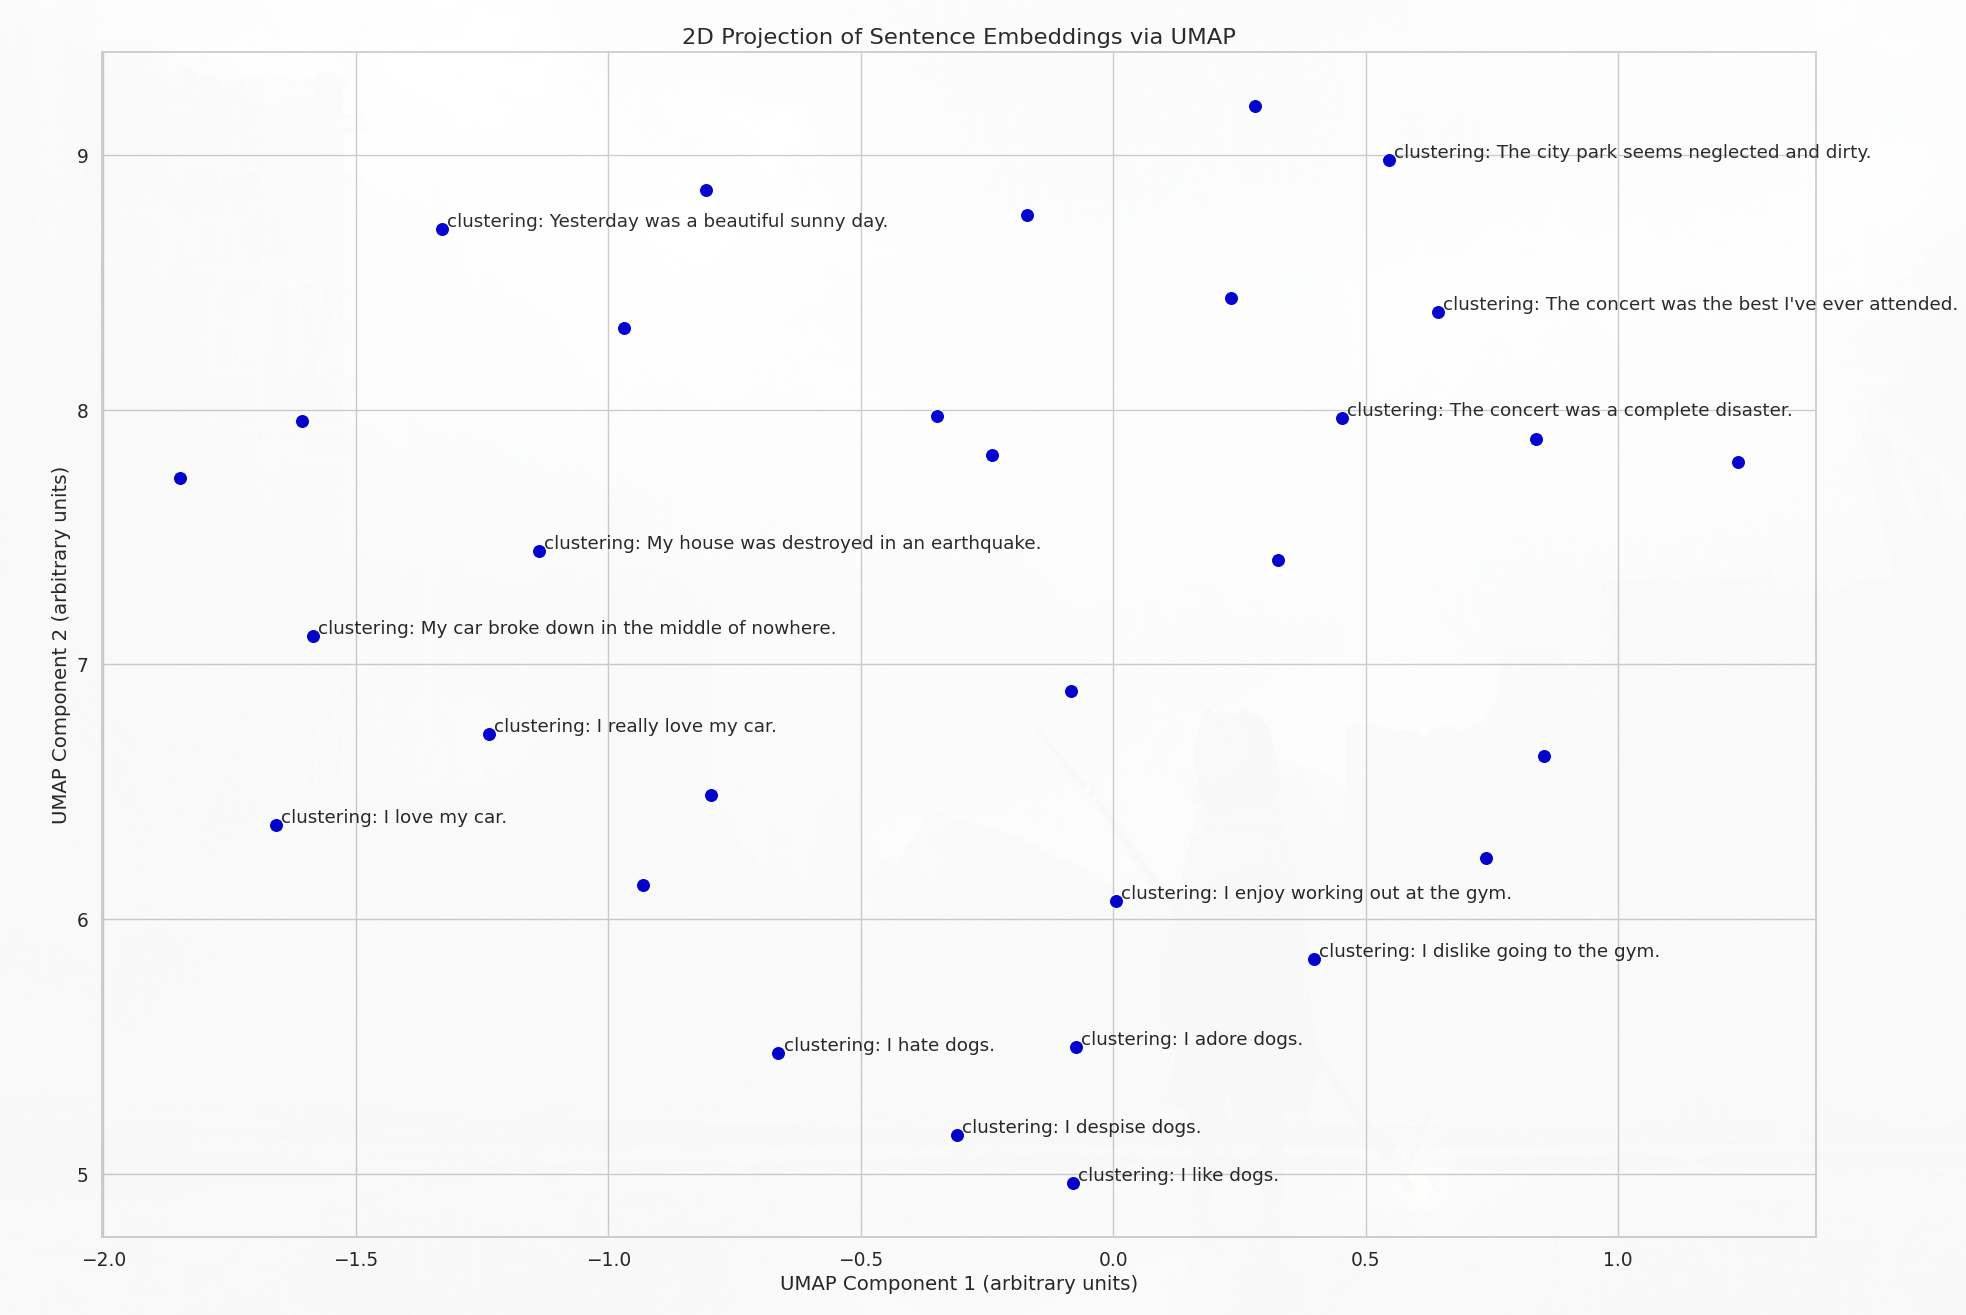
\includegraphics[width=0.95\textwidth]{sentenceEmbeddingExample.png}
    \caption{Example text embedding with Nomic Text Embedding v1.5 \cite{nussbaum2024nomic} of random sentences generated using OpenAI's ChatGPT o3-mini-high and projected onto 2 dimensions using UMAP \cite{mcinnes2018umap} with a random seed of 42 and minimum neighbours of 15. Only some of the labels are highlighted for visual clarity.}\label{fig:sentenceEmbeddingExample}
\end{figure}

\subsection{Transformers}\label{sec:BERT}
Pre-trained language models (PLMs), such as BERT \cite{devlin2019bert}, have been widely successful in a wide range of NLP tasks through fine-tuning \cite{edunov2019pre, min2023recent}. Fine-tuning is the process of re-training a PLM on specialised tasks, leveraging the model's base knowledge, by applying perturbations to the pre-trained model parameters through gradient descent learning algorithms. These language models, trained on finding an embedding space for natural language as well as stochastically generating tokens to mimic natural language, often provide a great platform to perform task-specific model fine-tuning. 
\todo{fix wording}
Platforms such as HuggingFace \cite{wolf2019huggingface}, allow authors to upload these pre-trained model parameters which in-turn allows researchers to download them for them fine-tuning. Moreover, task-specific fine-tuned models parameters are uploaded, downloaded and shared on these platforms. These fine-tuned models are useful for researchers whose focus lies outside of optimising these model parameters.
In this section, we talk about the transformer-family of language models.

\subsubsection{BERT}
The Bidirectional Encoder Representations from Transformer (BERT) language model introduced in 2018 by Google AI Language team in (\citet{devlin2019bert}) was designed to learn deep bidirectional representations from unlabelled text. It achieved this by learning the left and right context in every layer of the model. The model implementation can be split into two phases: \todo{sprinkle some images in here.} (1) the pre-training phase; and (2) the fine-tuning phase. This allows the model architecture to remain common, with many down-stream NLP tasks benefiting from a single PLM \cite{devlin2019bert}. An example illustration can be seen in Figure~\ref{fig:bert1}, where a single model can be fine-tuned on many down-stream tasks by simply replacing the output layer. The model architecture is a multi-layer transformer encoder based on the original paper (\citet{vaswani2017attention}) which is bidirectional by nature. As the transformer architecture is a very well researched architecture, well represented in the literature and slightly out-of-scope for this paper, we refer the reader to the original paper.

\begin{figure}[htbp]
    \centering
    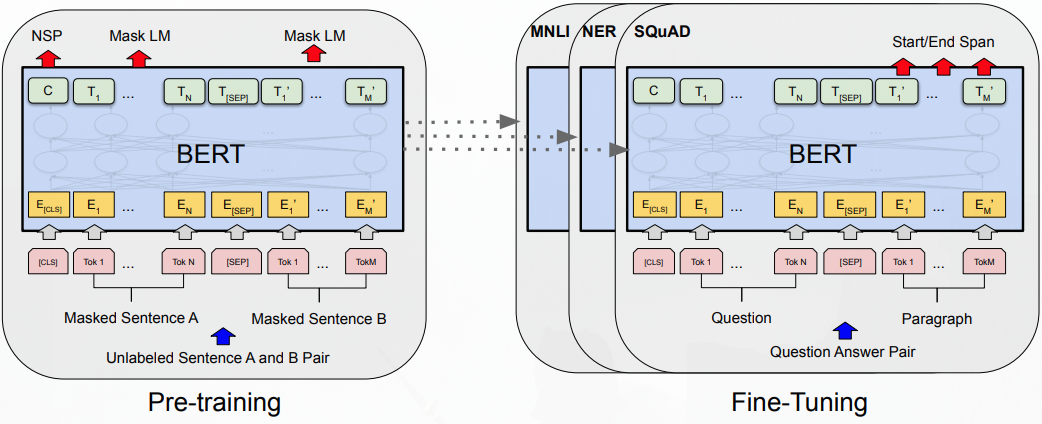
\includegraphics[width=0.95\textwidth]{BERT1.png}
    \caption{The overall pre-training and fine-tuning phases for BERT. For different down-stream tasks, notice the same architecture, except output layer, is used. Source: (\citet{devlin2019bert}).}\label{fig:bert1}
\end{figure}

\textbf{}\\ The pre-training phase can be split into two further training tasks (otherwise referred to as objectives):
\begin{itemize}
\item  Masked Language Modelling - During training, a portion of the input tokens are `masked' and the model predicts these masked tokens based on the remaining context, using cross-entropy loss \cite{zhang2018generalized}. In the literature, this is referred to as a Cloze task \cite{taylor1953cloze}. In the experiments conducted by (\citet{devlin2019bert}) 15\% of tokens in each sequence are randomly selected for masking. However, to mitigate the mismatch between pre-training and fine-tuning phases, a training data generator replaces each chosen masked tokens with: (1) the special token \texttt{[MASK]} 80\% of the time; (2) a random token 10\% of the time; and (3) the original token itself 10\% of the time \cite{devlin2019bert}.
    \item Next Sentence Prediction - In this task, the model is trained on a binary classification task prediction the relationship between sentence pairs. Given two sentences \texttt{A} and \texttt{B} either (1) sentence \texttt{B} is the actual sentence that follows \texttt{A} 50\% of the time or (2) sentence \texttt{B} is randomly selected from the corpus 50\% of the time \cite{devlin2019bert}. 
\end{itemize}

\textbf{}\\ The Google AI Language team further fine-tune BERT across 11 NLP tasks, showing that BERT out-performed the state-of-the-art models at its point in time.

As previously mentioned, a benefit of using PLMs such as BERT for NLP tasks (such as text embedding) is the ability to off-load the computationally intensive pre-training and any initial fine-tuning stages to another party. Although, this means that there now exists an implicit trust in that third-party's model parameters. For example, the third-party could be motivated by factors to censor certain phrases, artificially injecting testing data into training to increase performance metrics or maliciously change the embedding space. These are all factors which influence our decision on using a PLM and, thus, PLMs with transparently documented data sources, pre-training and fine-tuning should be preferred.

Since the release of the Google AI Language team's BERT, there have been some developments on further improving the performance of PLMs based on techniques presented in the paper. Namely, we touch on two: XLNet \cite{yang2019xlnet} and MPNet \cite{song2020mpnet}. 
XLNet's architecture is backed by the Transfomer-XL model \cite{dai2019transformer}. However, it is still briefly covered here to motivate MPNet. MPNet is a hybrid model that inherits XLNet's key feature, permutation language modelling, and BERT's masked language modelling, producing a `unified view'.

\subsubsection{XLNet}\label{sec:xlnet}

According to (\citet{yang2019xlnet}), the most successful pre-training objectives can broadly be split into two categories: (1) auto-regressive (AR) and auto-encoding (AE). AR language modelling, given a sequence of tokens $X = (x_1, ..., x_T)$, aims to factorize likelihood of a token into either a forward (Equation~\ref{eq:fwdprod}) or backward (Equation~\ref{eq:bckprod}) product. As an AR language model encodes context in a singular direction (only forward or backward, but not both), it has been shown to not be effective \cite{yang2019xlnet}. The notation $X_{<i}$ for some $1 \le i \le T$ means to include the first $i - 1$ elements (vice versa for $X_{>i}$).

\begin{align}
    p(x) &= \prod_{i=1}^{T} p(x_i | X_{<i})
    \label{eq:fwdprod} \\
    p(x) &= \prod_{i=T}^{i} p(x_i | X_{>i})
    \label{eq:bckprod}
\end{align}

AE language modelling, such as BERT, on the other hand aims to construct the original data from masked or malformed input, without estimations of the probability densities \cite{yang2019xlnet}. 
One downside of BERT, is the discrepancy between the pre-training and fine-tuning phases. Although BERT utilises bidirectional context for reconstruction of the special \texttt{[MASK]} token during pre-training, this special token does not exist at the fine-tuning phase. Additionally, the predicted tokens are masked in the \textit{input} and BERT assumes the predicted tokens are independent to the surrounding context as it is not able to model joint probabilities \cite{yang2019xlnet}. This assumption is an gross oversimplification, as longer term dependencies are highly prevalent in natural language applications \cite{schank1972conceptual, dai2019transformer}. 

Therefore, XLNet proposes an AR language modelling solution, backed by Transfomer-XL architecture \cite{dai2019transformer}, that combines the benefits of both AR and AE language modelling whilst avoiding their downsides. It does this by introducing two methods, described below.

\begin{itemize}
    \item{Permutation language modelling - XLNet maximises the pre-training objective, the expected log-likelihood over all possible factorisation orders of a length-$T$ sequence. A factorisation order is simply one way of shuffling the token positions $1, ..., T$. Imagine picking a shuffle then walking through the sentence in that order - when we come to a token, we predict it only using the tokens that appeared earlier in the very same shuffle even if those tokens lie to its right in the original sequence. Since this procedure is repeated for all shuffles, every token eventually `sees' information from both sides of the input, which gives XLNet a BERT-like bidirectional context \cite{yang2019xlnet}. More formally, 
            \begin{equation} \max_{\theta} \text{  } \mathbb{E}_{z\in\mathcal{Z}_T} \bigl[ \sum_{i=1}^{T} \log p_{\theta} \bigl(x_{z_i}\mid x_{z_{<i}}\bigr) \bigr], \label{eq:plm} \end{equation}
            where $\mathcal{Z_T}$ is the set of all $T!$ permutations of the index list $[1, ... , T]$. For a given permutation $z = (z_1, ..., z_T)$, $X_{z_{<i}}$ denotes the tokens that appear before $z_i$ in that permutation. $\theta$ denotes the model parameters, and is shared across all orders \cite{yang2019xlnet}.
        }

    \item{Two-stream self-attention - A naive transformer would expose the model to the very token it is trying to predict. XLNet avoids this by splitting the hidden state at every layer into (1) a content stream $h$, which encodes both content and position for every input token, and (2) a query stream $g$ which is target-aware. That is, the query stream knows where in the sequence a prediction is to be made, through its positional embedding but never sees the token's content \cite{vaswani2017attention, yang2019xlnet}. This helps the model use a different probability density depending on where in the text it is predicting, which BERT was lacking. At layer $m$ and target position $z_i$, the update sequence for $h$ and $g$ look like the following, using the regular attention function from (\citet{vaswani2017attention}), 
            \begin{align}
                g_{z_i}^{(m)} &\leftarrow \text{Attention} (Q = g_{z_i}^{(m - 1)}, KV = h_{z_{<i}}^{(m - 1)}) \\
                h_{z_i}^{(m)} &\leftarrow \text{Attention} (Q = h_{z_i}^{(m - 1)}, KV = h_{z_{\le i}}^{(m - 1)})
            \end{align}
            The query-stream vector $g_{(z_i)}^{(M)}$, after $M$ layers, is used to compute the soft-max \cite{gao2017properties} over some pre-determined vocabulary. This ensures the model predicts $x_{(z_i)}$ without ever having directly observed it. This is while the content stream continues to propagate contextual signals and positional signals.
        the use of two sets of hidden representations, the content representation and query representation. The content representation encodes both the context and the permutation $x_{(z_i)}$ whereas the query representation only encodes the position $z_i$ and the contextual information $X_{(Z_{<i})}$ \cite{yang2019xlnet}.}
\end{itemize}

Through integration of permutation language modelling and two-stream self-attention, XLNet inherits the probability density estimation ability of AR models and bidirectional context of AE models. Additionally, it also side-steps BERT's pre-train and fine-tune discrepancy and independence assumption \cite{yang2019xlnet}. For further specific details on XLNet, the reader is referred to (\citet{yang2019xlnet}).


% \todo{Finish this off (the caption)}


% \todo[inline, caption={}] {
%     \begin{itemize}
%         \item Mathematics of BERT (detailed in XLNet paper) - DONE
%         \item Mathematics of XLNet (detailed in XLNet paper) - DONE
%         \item Mathematics of MPNet (detailed in MPNet paper) - DONE
%         \item Autoregressive vs autoencoder - DONE
%         \item Architectural changes in XLNet - SKIPPED
%         \item Compare XLNet, MPNet and BERT.
%         \item Architectural differences from BERT to MPNet.
%     \end{itemize}
% }

\section{Dimensionality Reduction}\label{sec:dimred}

Embedding spaces can get large, often on the scale of hundreds or even thousands of embedding dimensions. For example, the BERT base architecture uses an embedding dimension of 768 \cite{devlin2019bert}. Therefore, in applications dealing with such embedding spaces, this motivates a technique that reduces the dimensions to 2- or 3-dimensions but reflects the high-dimensional characteristics of the dataset. 
Dimensionality reduction exploits the redundancy of the dataset by finding a smaller set of new features (variables) that are representative of the original data \cite{sorzano2014survey}.

It has been shown that many high-dimensional spaces show `counter-intuitive geometrical properties', impacting data analysis methods, such as clustering. This phenomenon is referred to as the `curse of dimensionality' \cite{verleysen2005curse, hinneburg1999optimal}. Further, most clustering algorithms (such as those described in Section~\ref{sec:clustering}) have been shown to be inefficient in high-dimensional spaces, due to this curse \cite{hinneburg1999optimal}. Thus, in order to apply clustering (as we will, later in Chapter~\ref{chap:Methodology}) dimensionality reduction is once again motivated.

This technique is not new in Statistics, with one of the most widely used dimensionality reduction techniques, Principal Component Analysis (PCA), introduced in (\citet{pearson1901liii}). However, with the increase in the quantity of available data and computational resources, researchers in fields such as Machine Learning and Statistics have developed a wide array of techniques aimed at tackling the dimensionality reduction problem \cite{sorzano2014survey}.

In this section, we cover the background required in understanding techniques used in Chapter~\ref{chap:Methodology}, Principal Component Analysis (PCA) and Uniform Manifold Approximation and Projection (UMAP).

% \todo[inline, caption={}] {
%     \begin{itemize}
%         \item Talk why dimensionality reduction is needed: visualisation, curse of dimensionality, clustering? Figure out how to structure this well for the story.
%         \item Talk about PCA and UMAP.
%     \end{itemize}
% }

\subsection{Principal Component Analysis}
Principal Component Analysis (PCA), as mentioned before, was first introduced in (\citet{pearson1901liii}) but later independently developed and named in (\citet{hotelling1933analysis}). PCA computes principal components, or variables which linearly decompose the features of the original dataset.
The core idea is to find directions (the principal components) in the data that capture the maximum amount of variance, essentially identifying the axes along which the data spreads out the most \cite{abdi2010principal}. Each subsequent principal component is computed to be orthogonal (that is, statistically uncorrelated) to the previous ones, ensuring that the new components capture different aspects of the data's variance.

This process can be described as an optimisation problem. Given a data matrix $X \in \mathbb{R}^{m \times n}$ (where $m$ is the number of data samples and $n$ is the number of original features), we want to find a new, lower-dimensional linear subspace, defined by the principal components, such that when the data $X$ is projected onto this subspace, the variance of the projected data is maximised. Equivalently, this can be viewed as finding the linear subspace that minimises the reconstruction error, specifically, the sum of squared distances (least-squares distance) between the original data points and their projections onto the subspace \cite{udell2016generalized}.

More formally, if we want to reduce the dimensionality from $n$ features down to $k$ principal components (for $k < n$), we seek a matrix $C \in \mathbb{R}^{n \times k}$ whose columns represent these top $k$ orthogonal component directions. The projected data in the lower $k$-dimensional space is given by $XC$. We can approximate the original data $X$ by projecting back from this lower dimension using $XCC^T$. PCA aims to find the matrix $C$ that minimises the difference between the original data $X$ and this reconstructed data $XCC^T$, subject to the constraint that the column-wise components are orthogonal ($C^TC = I$, for the identity matrix $I$) \cite{udell2016generalized}:
\begin{align}
    \min_C || X - XCC^T ||_F^2 
    \label{eq:pca} % Kept original label
\end{align}

A standard and efficient method for solving this optimisation problem and finding the principal components is through the Singular Value Decomposition (SVD) of the data matrix $X$ \cite{steinberger2005text, udell2016generalized}. SVD is a fundamental matrix factorisation technique that decomposes $X$ into three matrices:
\begin{align}
    X = USV^T \label{eq:svd} % Changed label to svd for clarity
\end{align}
Here, $U \in \mathbb{R}^{m \times k}$ and $V \in \mathbb{R}^{n \times k}$ are matrices with orthogonal columns, $S \in \mathbb{R}^{k \times k}$ is a diagonal matrix (only the diagonal contains non-zero elements) which contains the non-negative singular values ($s_i$) sorted in descending order, and $k$ is the rank of matrix $X$.

The crucial link to PCA is that the columns of the matrix $V$ are precisely the principal component directions we seek. That is, the matrix $C$ in Equation~\ref{eq:pca}, containing the top $k$ principal components, corresponds to the first $k$ columns of $V$.

Furthermore, SVD connects directly to the covariance matrix of the data ($X^TX$, assuming $X$ is centered). The decomposition of the covariance matrix is given by:
\begin{align}
    X^TX &= (USV^T)^T (USV^T) \\ % Show transpose step
         &= (VS^T U^T) (USV^T) \\ % Apply transpose rules
         &= V S^T (U^T U) S V^T \\ % Associativity
         &= V S^T I S V^T \quad \text{(since } U^T U = I \text{)} \\
         &= V (S^T S) V^T \\
         &= V S^2 V^T\quad \text{(since } S \text{ is a diagonal matrix)}
         \label{eq:svd_covariance} % Changed label, S^T S = S^2 as S is diagonal
\end{align}

This is the eigen-decomposition of the covariance matrix $X^TX$. It shows that the columns of $V$ are the eigenvectors (the principal components), and the diagonal entries of $S^2$  are the corresponding eigenvalues (i.e. $s_i^2 = \lambda_i$). Since the eigenvalues represent the variance of the data along the eigenvectors, the squared singular values ($s_i^2$) directly quantify the variance captured by each principal component \cite{udell2016generalized}. Therefore, computing the SVD of the data matrix $X$ provides both the principal components (in $V$) and the measure of variance associated with each component (in $S^2$) without explicitly forming the covariance matrix. Using a truncated SVD (keeping only the top $k$ components corresponding to the largest singular values) gives us a reduction in the dimensions.


% \todo[inline, caption={}] {
%     \begin{itemize}
%         \item Talk about PCA mathematics and why its used for dim reduction
%         \item Talk about elbowing and finding the most optimal (?)
%     \end{itemize}
% }

\subsection{Uniform Manifold Approximation and Projection}\label{sec:umap}

Unlike PCA, Uniform Manifold Approximation and Projection (UMAP) is generally considered a less directly interpretable dimensionality reduction method in terms of linear components. UMAP is a non-linear, stochastic `manifold learning technique' designed for dimensionality reduction, with theoretical foundations in Riemannian geometry and algebraic topology \cite{mcinnes2018umap}. As it places no constraints on the dimensionality of the input space, it is viable as a general-purpose technique in machine learning, often used for visualisation or as a pre-processing step for other algorithms like clustering. For the reader interested in the rigorous mathematics underpinning these topics, we refer them to the following textbooks: (1) (\citet{lee2003smooth}) for an introduction to differentiable and Riemannian manifolds; (2) (\citet{lee2006riemannian}) for Riemannian geometry in greater detail; and (3) (\citet{willard2012general}) for fundamental concepts of general topology.

The UMAP algorithm operates under the assumption that the high-dimensional data (the input embeddings in our case) lies on or near a lower-dimensional manifold embedded within the high-dimensional space. The algorithm then attempts to find a low-dimensional representation (typically 2- or 3-dimensional) that best models the essential structure of this assumed manifold. \\

\noindent Conceptually, the UMAP algorithm achieves this in two main stages \cite{mcinnes2018umap}:
\begin{enumerate}
    \item High-dimensional graph construction - First, UMAP constructs a representation of the relationships between data points in the original high-dimensional space. It does this by finding the nearest neighbours for each point and constructing a weighted graph where edge weights represent the estimated probability or likelihood that two points are closely connected on the underlying manifold. This step focuses on capturing the local structure and connectivity of the data.
    \item Low-dimensional layout optimization - Second, UMAP initialises the data points in the target low-dimensional space randomly. It then iteratively adjusts the positions of these low-dimensional points to create a graph structure that is as similar as possible to the high-dimensional graph constructed in the first stage. This optimisation process aims to minimise the difference (often measured using cross-entropy, a measure of divergence between probability distributions \cite{zhang2018generalized}) between the edge weights (probabilities of connection) in the high-dimensional and low-dimensional graphs. In other words, it tries to arrange the points in the low dimension such that connected points in the high dimension remain connected, and disconnected points remain disconnected.
\end{enumerate}

The outcome is a low-dimensional embedding that aims to preserve both the local connectivity structure and, to some extent, the broader global structure of the data's manifold. 

The output of the UMAP algorithm can be significantly influenced by several hyperparameters, which allow the user to tune the dimensionality reduction process \cite{mcinnes2018umap}. The two most commonly adjusted parameters are:
\begin{itemize}
    \item \texttt{n\_neighbors}: Determines the size of the local neighbourhood UMAP considers when initially modelling the manifold structure in the high-dimensional space. It controls the balance between capturing local detail versus preserving the global structure of the data. Lower values focus UMAP on very local structure, potentially isolating small, distinct groups but risking the loss of broader relationships. Higher values encourage UMAP to consider more points as neighbours, leading to embeddings that better reflect the overall global structure but may obscure fine-grained details or merge closely related clusters.
    \item \texttt{min\_dist}: This parameter controls the minimum distance between points in the final low-dimensional embedding space. It primarily affects the visual density of the resulting plot. Lower values allow points to be packed very tightly together, emphasizing cluster separation and density. Higher values force points further apart, creating more dispersed embeddings where the structure within potential clusters might be more visible, but the clusters themselves may appear less distinct.
    \item \texttt{n\_components}: This parameter specifies the target dimensionality of the reduced embedding space. It is commonly set to 2 or 3 for visualisation purposes, but can be set to higher values if the UMAP output is intended as input for subsequent machine learning tasks, such as clustering. Changing this directly alters the number of dimensions in the output array. 
    \item \texttt{metric}: This parameter defines the distance metric used to measure similarity or dissimilarity between data points in the original high-dimensional input space when finding nearest neighbours. The default is typically `euclidean', but other metrics like `cosine' (cosine distance) or `manhattan' (Manhattan distance) can be specified. The choice of metric is crucial and depends heavily on the nature of the input data. For instance, `cosine' distance is often preferred for high-dimensional, sparse data such as text embeddings, as it measures orientation rather than magnitude \cite{mcinnes2018umap}. Using an inappropriate metric can significantly distort the perceived local structure and thus the final embedding.
\end{itemize}

Selecting appropriate values for these parameters often involves experimentation based on the dataset and the specific goals of the dimensionality reduction (i.e. visualisation vs. input for clustering) \cite{mcinnes2018umap}. Implementations of UMAP, such as the widely used \texttt{umap-learn} Python library, are noted for being computationally efficient and scalable relative to other non-linear techniques like t-distributed Stochastic Neighbour Embedding (t-SNE) \cite{cai2022theoretical}, making UMAP a practical choice for many machine learning applications \cite{mcinnes2018umap}.

\begin{figure}[htbp]
    \centering
    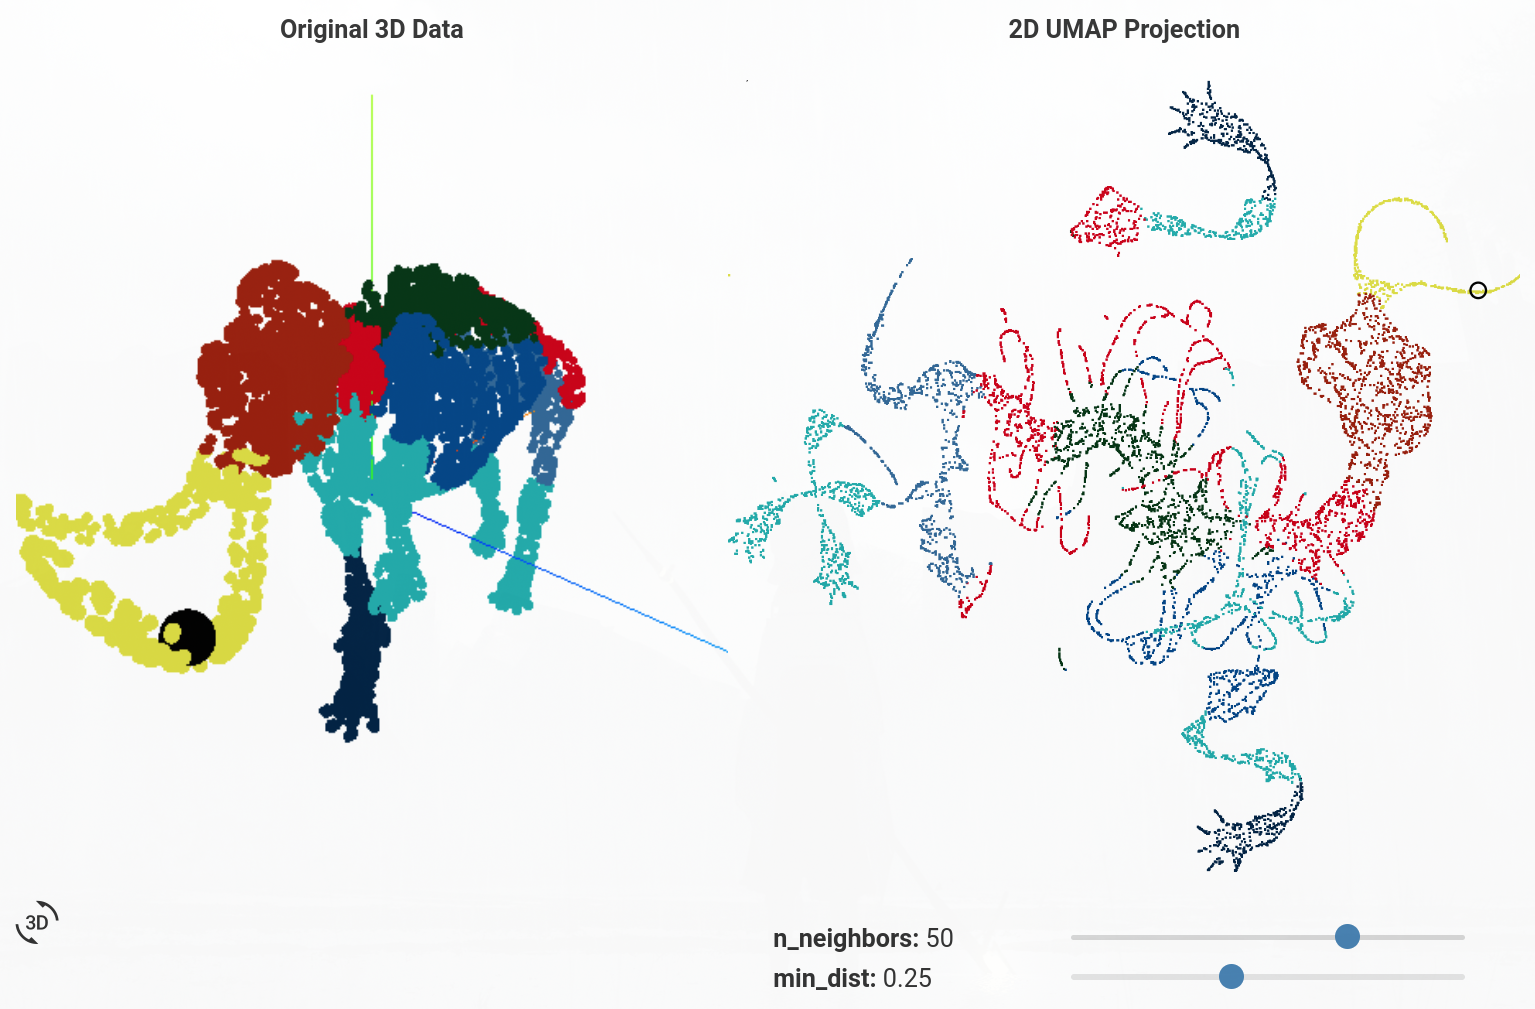
\includegraphics[width=0.6\textwidth]{./images/umapElephant.png}
    \caption{An illustration of UMAP applied (right) on samples taken from the skeletal structure of an elephant in 3-dimensions (left) with the UMAP hyperparameter values displayed. Highlighted, a black sphere (left) and circle (right), shows a chosen point mapped from 3-dimensions to 2. Source: (\citet{umapelephant}).}\label{fig:umapElephant}
\end{figure}

While powerful for visualisation and revealing non-linear structures, the resulting axes in the UMAP embedding do not have the same direct interpretation as the variance-ordered principal components derived from PCA.
An example illustration of UMAP applied to an elephant skeletal structure, which is considered structured data, can be seen in Figure~\ref{fig:umapElephant}.

% \todo[inline, caption={}] {
%     \begin{itemize}
%         \item Talk about UMAP, the algorithm, the assumptions, the constraints
%         \item Use the visualisation of the elephant here.
%     \end{itemize}
% }

\section{Clustering}\label{sec:clustering}

Clustering is an unsupervised machine learning task that aims to group data points such that items within a group (a cluster) are more similar to each other than to those in other clusters. Common approaches include partitioning methods, which divide the data into a predefined number of clusters, density-based methods, which identify clusters based on regions of high data point density, and hierarchical methods, which build a tree-like structure of nested clusters \cite{kaufman2009finding}.

This section provides the necessary background for the clustering techniques employed later in this project. We will cover k-Medoids \cite{kmedoids}, a partitioning algorithm; Density-Based Spatial Clustering of Applications with Noise (DBSCAN) \cite{ester1996density}, a density-based algorithm; and Hierarchical DBSCAN (HDBSCAN) \cite{campello2013density}, which builds upon density and hierarchical concepts.

% \todo[inline, caption={}] {
%     \begin{itemize}
%         \item Talk about what clustering does, i.e. looking at trying to categorise or something - DONE
%         \item Talk about the curse of dimensionality and why clustering does not perform well. Then talk about what people usually do (dimensionality reduction via feature selection or algorithms) - BEFORE
%         \item Talk about k-Medoids (supervised), DBSCAN and HDBSCAN (unsupervised). - DONE, but wrong classification here.
%     \end{itemize}
% }

\subsection{k-Medoids}\label{sec:kmedoids}
The k-Medoids algorithm is a partitioning-based clustering method that aims to divide a dataset into k distinct clusters. The k-Medoids algorithm uses actual data points, known as medoids, as the centres of its clusters. It aims to minimise a cost function based on the sum of pairwise dissimilarities (that is, distances) between each point and the medoid of the cluster it is labelled under \cite{kmedoids}.

A classical algorithm for implementing k-Medoids is Partitioning Around Medoids (PAM), introduced by (\citet{kmedoids}). PAM operates in two main phases:

\begin{enumerate}
    \item The build phase - An initial set of $k$ data points are seleceted as the starting medoids. This selection aims to establish a reasonable initial clustering by choosing points that are relatively central within potential groups that exists - minimising the initial total dissimilarity.
    \item The swap phase - This phase iteratively refines the set of medoids. For each currently selected medoid $m$ and each non-medoid point data point $x$, the algorithm computes the change in total dissimilarity that would result from swapping $m$ and $x$. That is, setting $x$ as that centroid of $m$'s cluster. The swap that yields the greatest reduction across all possible pairs is finally performed. This process repeats until no swap can further reduce the total dissimilarity which indicates a local optimum has been reached.
\end{enumerate}

The PAM algorithm employs a greedy search strategy during the swap phase, which means it may converge to a local rather than a global optimum \cite{kmedoids}. The computational complexity of the SWAP phase is often cited as $O(k(n - k)^2)$ per iteration, where $n$ is the number of data points and $k$ is the number of clusters \cite{kmedoids}.

Algorithm~\ref{alg:pam} provides a high-level pseudocode description of the relatively straightforward PAM process. It takes the desired number of clusters $k$ and the dataset $X$ as input, and outputs the final set of medoids $M$ and set of clusters $X'$. The fact that $k$ is a parameter to the algorithm means that either the number of clusters must be known beforehand or must be found through hyperparameter optimisation.

% --- The Algorithm ---
\begin{algorithm}[caption={Partitioning Around Medoids (PAM).}, label={alg:pam}]
input: Dataset $X = \{x_1, ..., x_n\}$, integer $k$ (number of clusters)
output: Set of $k$ medoids $M$, Partition $X' = \{C_1, ..., C_k\}$ where $C_j$ is the set of points assigned to medoid $m_j$

begin
    # --- Build Phase (Conceptual) ---
    # Select an initial set of k medoids M from X
    # (i.e. using a heuristic that minimizes initial total dissimilarity)
    $M \gets$ SelectInitialMedoids($X, k$)

    # --- Swap Phase ---
    repeat
        best_cost_reduction $\gets 0$
        best_swap $\gets \emptyset$ 
        total_cost $\gets$ ComputeTotalDissimilarity($X, M$) # Cost based on current M

        # Consider swapping each medoid m with each non-medoid x
        foreach $m \in M$ do
            foreach $x \in X \setminus M$ do
                # Compute cost if m is replaced by x
                $M_{swap} \gets (M \setminus \{m\}) \cup \{x\}$
                cost_after_swap $\gets$ ComputeTotalDissimilarity($X, M_{swap}$)
                cost_reduction $\gets$ total_cost - cost_after_swap

                # Check if this swap is the best found so far
                if cost_reduction > best_cost_reduction then
                    best_cost_reduction $\gets$ cost_reduction
                    best_swap $\gets (m, x)$ # Store the potential swap pair
                end
            end
        end

        # Perform the best swap found in this iteration, if any cost reduction occurred
        if best_cost_reduction > 0 then
            ($m_{out}, x_{in}$) $\gets$ best_swap
            $M \gets (M \setminus \{m_{out}\}) \cup \{x_{in}\}$ # Update medoid set
            improved $\gets$ true
        else
            improved $\gets$ false # No cost reduction possible
        end
    until not improved # Stop when no swap improves the total cost

    # Assign points to final medoids to form clusters X'
    $X' \gets$ AssignPointsToClusters($X, M$)

    return M, X'
end
\end{algorithm}

% \todo[inline, caption={}] {
%     \begin{itemize}
%         \item Talk about algorithm
%         \item Talk about the parameters any effects when tuning these parameters.
%         \item Talk about drawbacks and benefits of this approach, citations needed.
%     \end{itemize}
% }

\subsection{DBSCAN}\ref{sec:dbscan}

Density-Based Spatial Clustering of Applications with Noise (DBSCAN) is density-based clustering algorithm, unlike partitioning methods like k-Medoids \cite{ester1996density}. Instead of partitioning data around centres, DBSCAN groups together points that are closely packed in high-density regions, separated by sparser areas. A key characteristic of this approach is its ability to discover clusters of arbitrary shapes and to automatically determine the number of clusters present, rather than requiring it as a predefined input \cite{ester1996density}. The core intuition is that points belonging to the same conceptual group or category tend to lie close to each other, forming denser regions than considered noise or outliers.

The algorithm's behaviour and the concept of density is controlled by two hyperparameters \cite{ester1996density}:
\begin{itemize}
    \item \texttt{Eps} - This parameter defines the maximum distance between two points for one to be considered as in the neighbourhood of the other. It essentially sets the radius for identifying neighbours. A smaller \texttt{Eps} value requires points to be closer together to form a dense region, potentially leading to smaller, tighter clusters and classifying more points as noise. Conversely, a larger \texttt{Eps} value allows clusters to span sparser regions and potentially merge groups that might otherwise be distinct.
    \item \texttt{MinPts} - This parameter specifies the minimum number of points (including the point itself) required within a point's Eps-neighbourhood for that point to be considered a core point (i.e. an interior point of a dense region). \text{MinPts} defines the threshold for density. A higher value requires more points to constitute a dense core, potentially resulting in fewer clusters and more points being classified as noise. A lower value allows sparser groupings to qualify as clusters, potentially resulting in more clusters.
\end{itemize}

Determining appropriate values for \texttt{Eps} and \texttt{MinPts} often requires a heuristic (such as the one described by (\citet{ester1996density})) or domain knowledge, as DBSCAN is an unsupervised machine learning algorithm \cite{ester1996density}.

To understand the algorithm's operation, several core concepts are essential \cite{ester1996density} \begin{itemize}
    \item Eps-neighbourhood - The Eps-neighbourhood of a point is the area within a radius of length \texttt{Eps} from that point.
    \item Density-reachable - A point $p$ is density reachable from another core point, if there is a sequence of points from $p$ to $q$ where the distance between any two points is less than or equal to \texttt{Eps} and every point in this sequence except $q$ must be a core point. This defines a chain of density connecting $p$ to $q$.
\end{itemize}

Additionally, based on the hyperparameters, DBSCAN categorises each point in the dataset into one of the three types \cite{ester1996density}. 
\begin{itemize}
    \item Core point - A point whose Eps-neighbourhood contains at least \texttt{MinPts} points, including itself. Core points are considered to be in the interior of a dense cluster.
    \item Border point - A point that is not a core point itself, but falls within the Eps-neighbourhood of at least one core point. Border points lie on the border of a cluster.
    \item Noise point - A point that is neither a core point nor a border point. These points typically reside in low-density regions and are not assigned to any cluster.
\end{itemize}

The DBSCAN algorithm, formally defined in (\citet{ester1996density}), iterates through the data points. When it encounters an unvisited point, it checks if that point qualifies as a core point by examining the set of points Eps-neighbourhood. If it is indeed a core point, then a new cluster is formed. This cluster is then expanded by finding all density-reachable points, starting from this initial core points. This involves recursively exploring the Eps-neighbourhood of all core points found during the expansion process. Any point reachable through a chain of core points connected by their Eps-neighbourhood becomes part of the cluster. If an unvisited point examined is not a core point, it is initially marked as noise, although it may be later reclassified as a border point, if found within the Eps-neighbourhood of a core point belonging to an expanding cluster. Points identified as density-reachable but not core points become border points assigned to this cluster. This procedure continues until all points in the dataset have been visited and assigned to a cluster or designated as noise.

An important consideration arises when a border point falls within the Eps-neighbourhood of core points belonging to different, simultaneously expanding clusters. Standard DBSCAN implementations typically resolve this based on the order of processing: the border point is assigned to the cluster associated with the first core point that `discovers' it during expansion \cite{ester1996density}. Once assigned, it is generally not reassigned, even if subsequently found to be reachable from another cluster's core point. Thus, while the core cluster structures are stable, the assignment of some border points can be implementation-dependent.

In general, DBSCAN offers significant advantages: it can identify clusters of arbitrary shape, is inherently robust to noise (which it explicitly labels) and does not require the number of clusters to be specified beforehand. However, it also has limitations. The algorithm's performance is sensitive to the choice of \texttt{Eps} and \texttt{MinPts} and it can struggle to correctly identify clusters of significantly varying densities within the same dataset. Furthermore, the average runtime complexity is $O(n\log n)$ where $n$ is the number of points in the dataset. \cite{ester1996density, campello2013density}. Like many distance-based algorithms, its effectiveness can degrade in very high-dimensional spaces due to the `curse of dimensionality' (see Section~\ref{sec:dimred}) \cite{hinneburg1999optimal, verleysen2005curse}.


% \todo[inline, caption={}] {
%     \begin{itemize}
%         \item Talk about algorithm
%         \item Talk about the parameters any effects when tuning these parameters.
%         \item Talk about drawbacks and benefits of this approach, citations needed.
%     \end{itemize}
% }

\subsection{HDBSCAN}\ref{sec:hdbscan}

Hierarchical Density-Based Spatial Clustering of Applications with Noise (HDBSCAN), proposed by \citet{campello2013density}, is an advancement over DBSCAN that generates a hierarchical clustering structure. This approach addresses a key limitation of DBSCAN: its reliance on a single global density threshold $\epsilon$ (equivalent to \texttt{Eps} in DBSCAN), which makes it difficult to identify clusters of varying densities simultaneously. HDBSCAN overcomes this by effectively exploring all possible density thresholds ($\lambda = \frac 1 \epsilon$, for all $\epsilon \in \big[0, \infty \big)$) to build a cluster hierarchy \cite{campello2013density}.

The method introduces two main contributions: (1) the HDBSCAN algorithm itself, which constructs this complete density-based hierarchy, represented as a dendrogram (a hierarchical tree-based representation of the dataset points); and (2) a novel measure of cluster stability used to extract a simplified, flat partition containing only the most significant and persistent clusters from this hierarchy \cite{campello2013density}. This extraction is framed as an optimisation problem maximising the total stability of the selected clusters. A significant advantage of HDBSCAN is its reduced sensitivity to hyperparameters as it primarily requires only $m_{\text{pts}}$ (equivalent to \texttt{MinPts} in DBSCAN), a parameter whose effect as a density smoothing factor is generally well-understood \cite{campello2013density}.

Importantly, the remaining portion of this section assumes a reasonably basic level of understanding of graph theory. For a great primer, the reader is referred to (\citet{harris2008combinatorics}).

To establish a formal link between the flat clustering of DBSCAN and the hierarchy of HDBSCAN, the authors first revisit the DBSCAN concept (referred to as DBSCAN\* in the paper for clarity). In this view, clusters are defined as connected components of core objects within a graph where edges connect mutually reachable core points based on $\epsilon$ and $m_{\text{pts}}$. Non-core objects are considered noise, which includes border points. This perspective allows density-based clusters to be seen as connected components of a level set of density (i.e. here, given a density threshold $\lambda = \frac 1 \epsilon$, it can be thought of as a set with points with density above that value) \cite{campello2013density}.

HDBSCAN builds upon the defining concepts relative to $m_{\text{pts}}$, only allowing $\epsilon$ (or $\lambda$) to vary \cite{campello2013density}:
\begin{itemize}
    \item Core distance ($d_{\text{core}}(x)$) - For a data point $x$, this is the distance to its $m_{\text{pts}}$-th nearest neighbour (including itself). It serves as a measure of the local density around $x$. A smaller core distance implies a denser region.
    \item Mutual reachability distance ($d_{\text{mreach}}(x_p, x_q)$) - Defined for two data points $x_p, x_q$, this is the maximum of their respective core distances and their pairwise distance defined as:
        \[d_{\text{mreach}}(x_p, x_q) = \max \{ d_{\text{core}}(x_p), d_{\text{core}}(x_q), d(x_p, x_q) \}\]
    This adjusted distance measure ensures that points in sparse regions are effectively pushed further apart, reflecting density differences.
\end{itemize}

The HDBSCAN algorithm constructs the cluster hierarchy based on these concepts. Conceptually, it first computes the core distance for all points. Then, it builds a graph where all points are vertices, and the weight of the edge between any two points is their mutual reachability distance. The algorithm finds the Minimum Spanning Tree (MST) of this complete graph. The cluster hierarchy (dendrogram) is then extracted from this MST by considering edges in decreasing order of weight (distance). As edges are removed (corresponding to decreasing the density threshold $\lambda$ or increasing the distance threshold $\epsilon$), connected components in the remaining graph represent clusters at that specific density level. The hierarchy captures how these components merge as the density threshold decreases \cite{campello2013density}. This process can be implemented efficiently, with a typical time complexity of $O(n^2)$ if pairwise distances are precomputed or provided, or potentially $O(dn^2)$ depending on MST construction details if distances are computed on the fly from $d$-dimensional data \cite{campello2013density}.

To extract a meaningful flat partition from this hierarchy, HDBSCAN introduces the concept of cluster stability. This measure quantifies how persistent a cluster $C_i$ is across different density levels ($\lambda = \frac 1 \epsilon$). That is, as you vary the density level $\lambda$, what is the longest period in which the cluster exists without disappear or splitting. The stability $S(C_i)$ is calculated by summing, for each point $x_j$ belonging to cluster $C_i$, the range of density levels for which that point remains part of that specific cluster \cite{campello2013density}. More formally, using the notation from the paper where $\lambda_{\text{min}}(C_i)$ is the density level at which cluster $C_i$ appears (thought of as is `born') and $\lambda_{\text{max}}(x_j, C_i)$ is the density at which point $x_j$ leaves cluster $C_i$, either through becoming noise or part of some child cluster as density increases \cite{campello2013density}:

\begin{align}
S(C_i) = \sum_{x_j \in C_i} (\lambda_{\text{max}}(x_j, C_i) - \lambda_{\text{min}}(C_i))
\label{eq:hdbscan-stability}
\end{align}

Equation~\ref{eq:hdbscan-stability} adapts the concept of `excess of mass' \cite{muller1991excess} to a set of discrete data points and density levels derived from the hierarchy. Clusters where points persist over a larger range of $\lambda$ values (i.e. are more `stable' across varying density thresholds) will have higher stability scores.

Using this concept of stability, HDBSCAN selects the optimal flat clustering by solving an optimisation problem: finding a maximal disjoint set of clusters from the hierarchy  such that the sum of stabilities $S(C_i)$ is maximised. Here a maximal disjoint set of clusters refers to the fact that no two cluster is an ancestor or descendant of another selected cluster, ensuring a flat partition covering all points down certain branches \cite{campello2013density}. The paper provides an efficient algorithm that traverses the simplified cluster tree bottom-up and then top-down to find this optimal set of stable clusters in linear time, relative to the size of the simplified tree. The simplified cluster tree is obtained after applying a minimum cluster size $m_{\text{dSize}}$, typically set equal to $m_{\text{pts}}$. This process effectively performs the optimal `local cuts' in the cluster dendrogram at different levels of hierarchy, based on this notion of cluster persistence.

\section{Clustering Evaluation}\label{sec:clusteringEval}
\todo[inline] {Maybe this can be moved to the methodology?}
Furthermore, as evaluating the quality of unsupervised clustering results is crucial, we will also introduce several common clustering evaluation heuristics used in this work: Inertia, the Silhouette coefficient \cite{rousseeuw1987silhouettes}, the Davies-Bouldin Index \cite{davies1979cluster}, and the Calinski-Harabasz Index \cite{calinski1974dendrite}.

\todo[inline, caption={}] {

    Maybe this should be later on in the methodology? 

    \begin{itemize}
        \item Motivate the need for clustering evaluation.
        \item Just highlight mathematics of each algorithm and mention the need for them.
    \end{itemize}
}
\subsection{Inertia}
\subsection{Silhouette}
\subsection{Davies-Bouldin Index}
\subsection{Calinski-Harabasz Index}

\section{Maybe Optuna}

\chapter{Automatic Categorisation and Label Generation}\label{chap:Methodology}

\section{Data}

Data relevant to the operational state and maintenance of the ISIS facility originates from several sources. The facility publishes open-access datasets, primarily containing instrument calibrations and experimental metrics, via its data portal \citep{isisdata}. Alongside this, the ISIS team maintains proprietary internal datasets detailing specific component performance, which are available upon request. For this research, access was granted to historical logs for the ion source component, with entries dating back to 27 March 2003. Furthermore, the operations crew maintains a daily operational log, the Operalog, documenting facility faults and the corresponding remedial actions taken.

Given the breadth of available data and the project's scope constraints, a decision was made to focus the analysis presented in this paper on the \textbf{Operalog}. This dataset provides a rich textual record of real-world failures across the facility, offering valuable insights despite its partially unstructured nature. Data from the specialised ion source logs is the focus of the partner project. 

\subsection{The Operalog}
The operational log, otherwise referred to as the `Operalog', is an Excel spreadsheet with entries documenting moments of machinery failure within the ISIS facility covering the period 1996 - 2023. Table~\ref{tab:operalog} documents the important features. Notably, the day-to-day operational crew have developed custom abbreviations, acronyms and terminology which may not immediately be clear. Additionally, different crew members have varying writing styles and levels of depth of information. Thus, this results in an unstructured text dataset which has a huge variance in quality and quantity of information. Furthermore, as noted in Table~\ref{tab:operalog}, \texttt{FaultRepair} was seemingly made redundant post-2017. Figure~\ref{fig:FaultDescriptionVSFaultRepairs} highlights the distribution in the text lengths of both unstructured text fields. Furthermore, around $0.02\%$ of \texttt{FaultDescription} fields are empty whereas around $66\%$ of \texttt{FaultRepair} fields are empty. The generally shorter entries in \texttt{FaultRepair}, with a large majority having fewer than or equal to 5 characters, suggest lower informational content compared to \texttt{FaultDescription}. This is further illustrated in the Wordcloud illustrations \cite{oesper2011wordcloud} (Figure~\ref{fig:wc}), where \texttt{FaultRepair} only has one extremely large word (`reset'). As the size of the word indicates the frequency, this means \texttt{FaultRepair} has the word `reset' in almost all non-empty entries. With `reset' being exactly 5 characters and most non-empty entries in \texttt{FaultRepair} being at most 5 characters (of which, those that contain reset are over 70\% of entries), it is easy to see that the \texttt{FaultDescription} field contains richer, more informative context. 

\rowcolors{2}{gray!10}{white}
\begin{table}[htbp]
    \fontsize{8}{11}\selectfont
    \centering
    \begin{adjustbox}{max width=\textwidth}
    \begin{tabular}{p{3cm} p{3cm} p{7cm}}
        \toprule
        \textbf{Feature Name} & \textbf{Data Type} & \textbf{Description} \\
        \midrule
        FaultDate & Date-time & Date the fault occurred, with a precision up to the nearest second. \\
        UserRun & String & Operational cycle that this fault has occurred within. Cycle information up to 2016 can be found at (\citet{isisbeamoperations2024}). \\
        Downtime & Integer & The amount of time, in hours the downtime has occurred for. \\
        Group & String, Fixed Category & The group that the faulty equipment is part of. There are 13 unique equipment groups. \\
        Equipment & String, Fixed Category & The equipment type that failed. There are around 200 unique equipment types that have been logged to fail. \\
        FaultDescription & String, Free-form & This is a free-form, unstructured text field that allows the on-shift operational crew to note details about the problem diagnosis and remediation that has occurred. There is no constraint to the size of this text field.\\
        FaultRepair & String, Free-form & Another free-form, unstructured text field that allows the on-shift operational crew to note only the remediation steps. The crew seems to have stopped using this field after the end of 2017, preferring to put remediation steps in FaultDescription. \\
        ManagersComments & String, Free-form & A very rarely used free-form text field, where the manager in charge of the on-shift crew will input comments. \\
        \bottomrule
    \end{tabular}
    \end{adjustbox}
    \caption{Description of important features (columns) in the Operalog.}
    \label{tab:operalog}
\end{table}

\begin{figure}[htbp]
    \centering
    \begin{subfigure}[b]{0.48\textwidth}
        \centering
        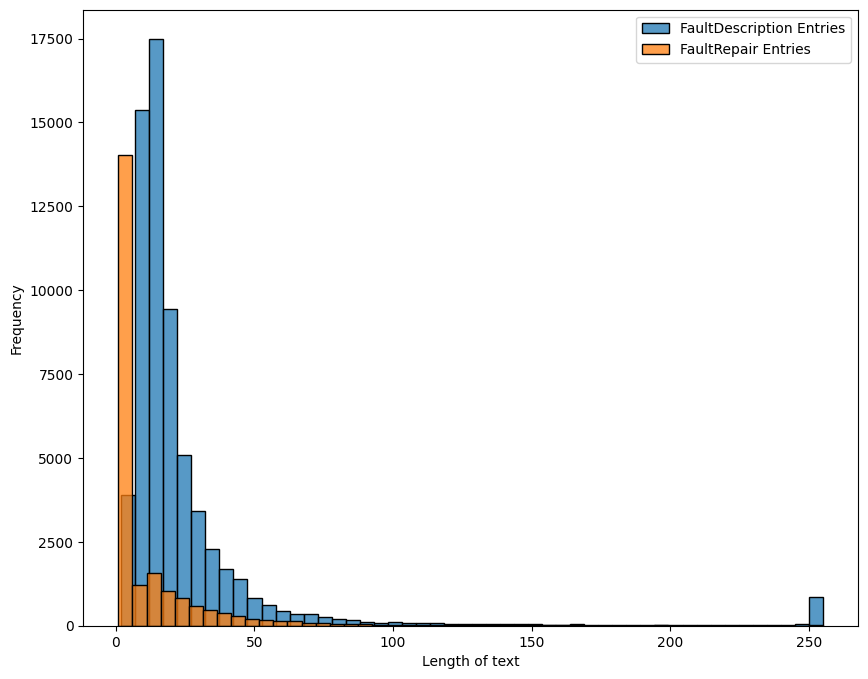
\includegraphics[width=\textwidth]{FaultDescriptionVSFaultRepairs.png}
        \caption{Frequency distribution of the text lengths for non-blank \texttt{FaultDescription} and \texttt{FaultRepair} fields. Each bar represents a range of 5 characters.}\label{fig:FaultDescriptionVSFaultRepairs}
    \end{subfigure}
    \hfill
    \begin{subfigure}[b]{0.48\textwidth}
        \centering
        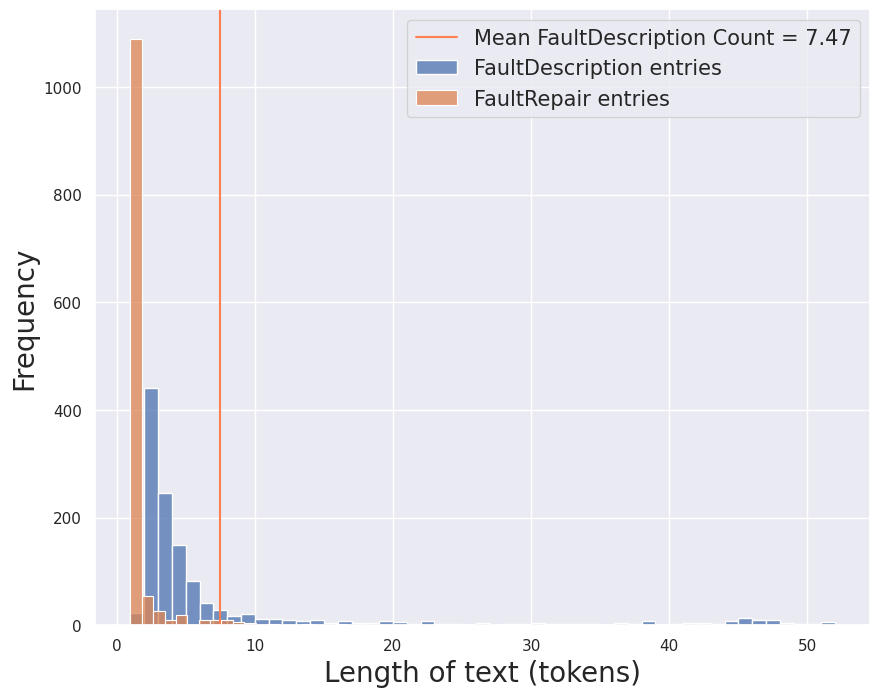
\includegraphics[width=\textwidth]{./images/ionSourceTokenCountDist.png}
        \caption{Frequency distribution of the number of tokens for non-blank \texttt{FaultDescription} and \texttt{FaultRepair} entries. Each bar represents a range of around 2 tokens.}\label{fig:ionSourceTokenCountDist}
    \end{subfigure}
    \caption{Frequency distributions of characters and tokens.}
    \label{fig:hists}
\end{figure}

\begin{figure}[htbp]
    \centering
    \begin{subfigure}[b]{0.48\textwidth}
        \centering
        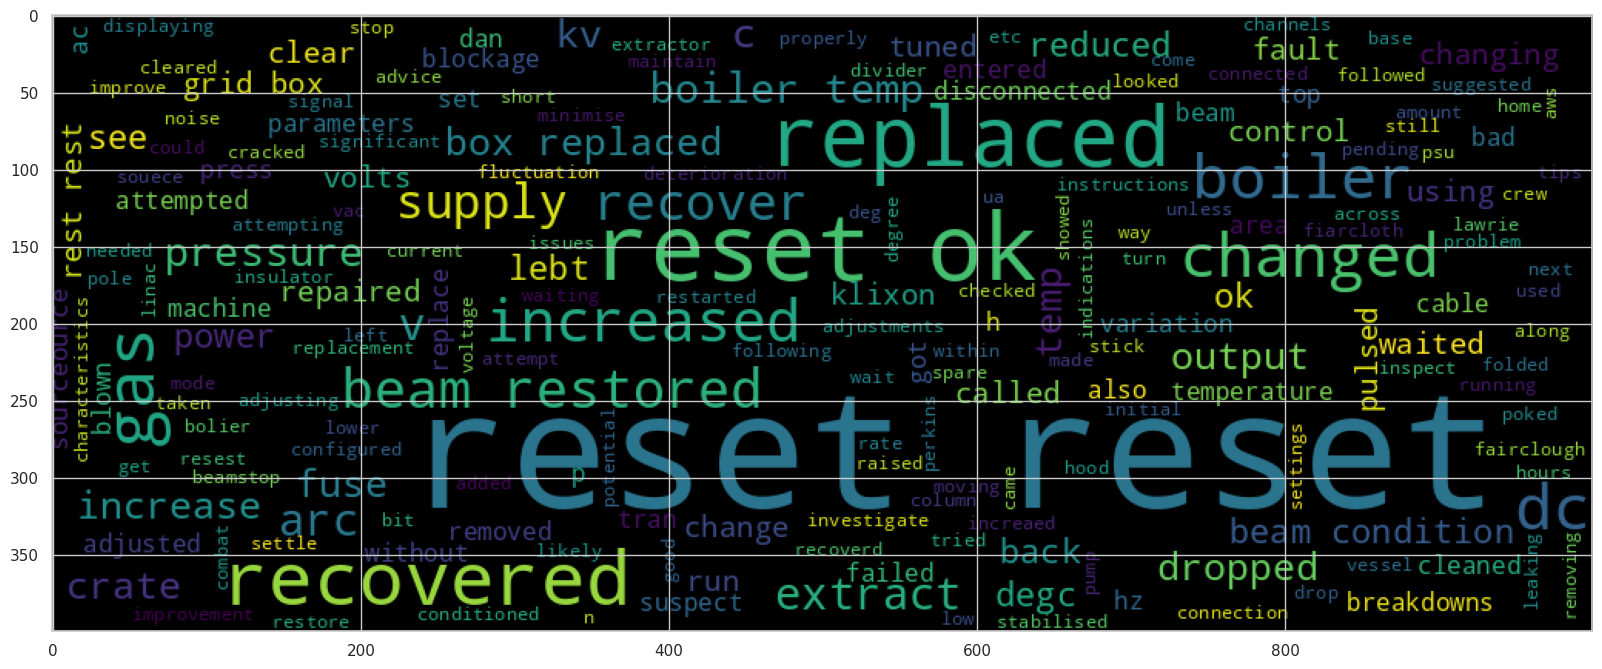
\includegraphics[width=\textwidth]{wcFaultRepairs.png}
        \caption{FaultRepair}
        \label{fig:wcFaultRepairs}
    \end{subfigure}%
    \hfill
    \begin{subfigure}[b]{0.48\textwidth}
        \centering
        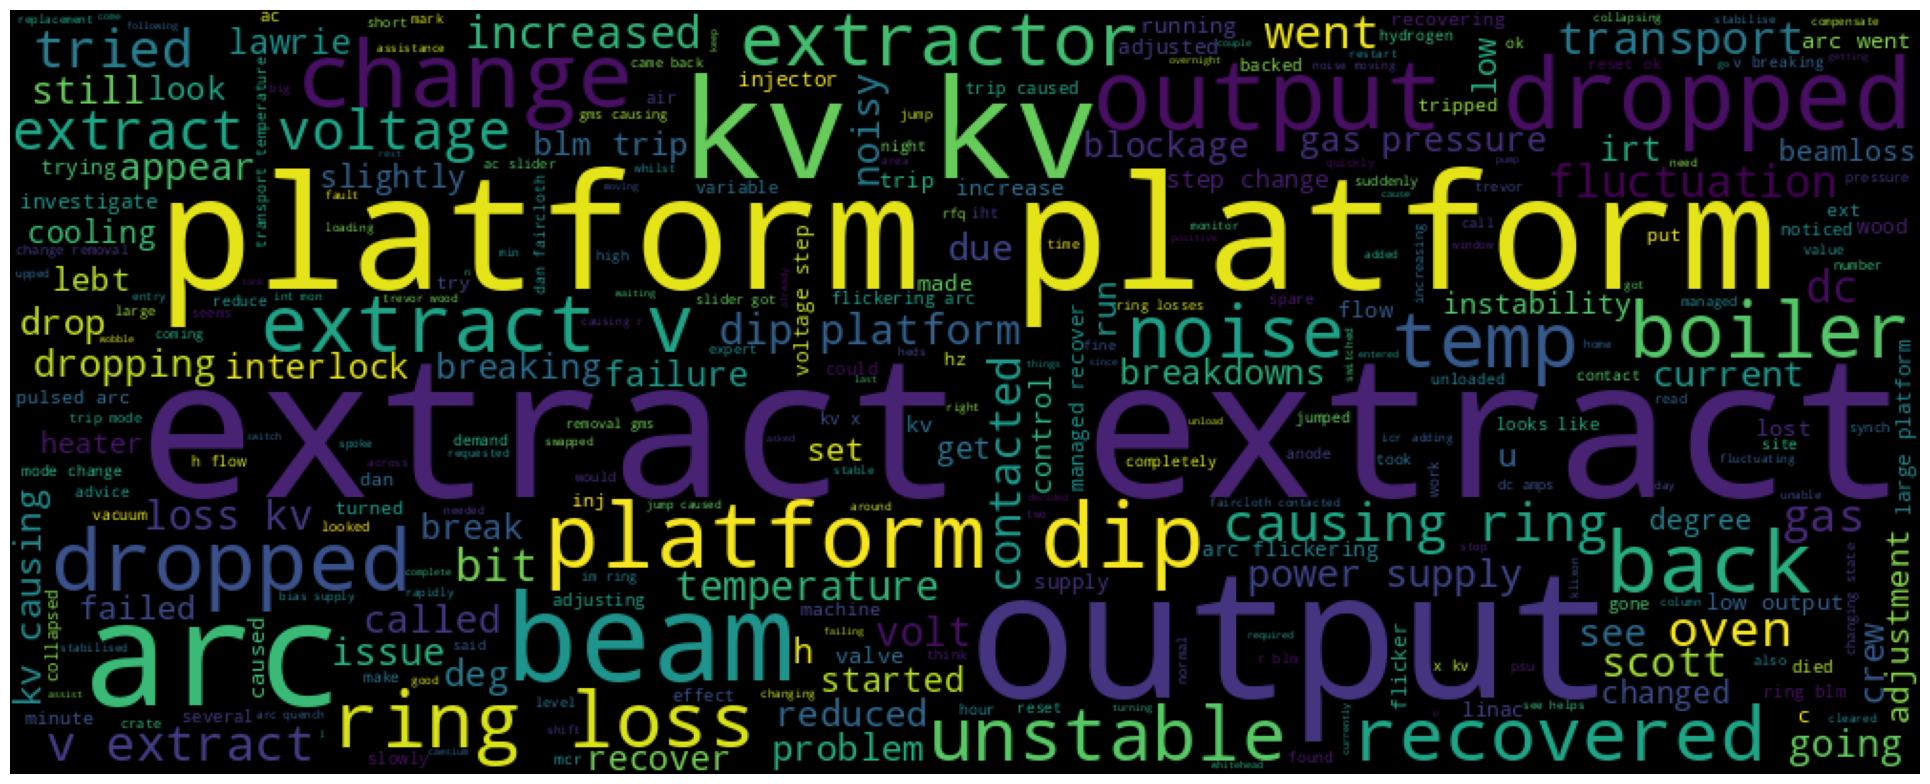
\includegraphics[width=\textwidth]{wcFaultDescription.png}
        \caption{FaultDescription}
        \label{fig:wcFaultDescription}
    \end{subfigure}
    \caption{Comparison of word clouds for the top 300 most common words for the FaultRepair field versus the FaultDescription field. Larger words are more common and collocations are enabled so both words and phrases are shown, leading to some repeating.}
    \label{fig:wc}
\end{figure}

\subsection{Preliminary Data Analysis}
\todo[inline, caption={}]{ 
    \begin{itemize}
        \item Talk about amount of issues per year
        \item Talk about the distribution of text lengths across whole df
        \item Talk about the distribution of text lengths across iondf
    \end{itemize}
}


\section{Overview}

\todo{Make a diagram that showcases the process (and all the hyperparameter choices)}

The process of transforming an unlabelled, uninformative Operalog into an informed, induced-label tagged dataset can be broadly characterised into five major steps. These steps are: (1) initial pre-processing and normalisation of the \texttt{FaultDescription} natural language text to standardise text and reduce noise; (2) embedding the cleaned text into a high-dimensional embedding space to capture semantic meaning numerically; (3) low-dimensional projection of the embedding space while respecting the higher-dimensional topological manifold (that is, aiming to preserve the structure and relationships present in the original high-dimensional space) to enable effective clustering while preserving structure; (4) performing clustering on the low-dimensional data, optimising clustering using clustering metrics as heuristics for the `goodness' of a cluster to group similar fault descriptions automatically; and (5) using natural language processing to induce label names for each cluster and tagging each entry with a meaningful label identifying a fault category.  Here, we choose to solely consider the \texttt{FaultDescription} field as the vast majority of \texttt{FaultRepair} fields are either empty or less than or equal to 5 characters long. 

Several hyperparameters affect the performance of the label generating process. Examples include model or algorithm specific parameters (i.e. the dimensionality reduction or clustering algorithms) and clustering `goodness' heuristics used. These hyperparameters are tuned using Optuna \cite{akiba2019optuna}, an automatic optimisation framework specifically designed for machine learning applications and allows for multi-objective optimisation. This hyperparameter optimisation process determines `best' induced categories, and thus labels, for each issue type. 

Additionally, as this project is an early stage exploration of auto-categorisation for the ISIS Operalog, the major focus is on ion source \texttt{Equipment} type unless explicitly specified. This enables the project to focus on refining the approach in a scoped manner with a structured goal in mind - to progress the auto-categorisation effort on the ISIS Operalog. The subsequent sections of this chapter detail each stage of this end-to-end pipeline, developed with the goal of producing an effective auto-categorisation model for the Operalog data.

\todo{Clean up wording in the above}

\section{Natural Language Pre-processing}

The aim of pre-processing the unstructured, English natural language text data from \\ \texttt{FaultDescription} is to normalise and prepare it for text embedding. Normalisation allows many syntactic permutations or augmentations of a text to be collapsed into one standardised form. This allows for consistent results as it ensures texts that are syntactically different but semantically similar will be mapped by embedding model to the same value. For pre-processing, and the rest of the pipeline, each log entry's \texttt{FaultDescription} is considered one text.

\todo{Clean up wording in the above}

Tokenisation is one of the earliest stages of natural language processing. To perform tokenisation, we use Tensorflow's \texttt{UnicodeScriptTokenizer} \cite{tensorflow2015whitepaper}. Tensorflow is `an end-to-end platform for machine learning', which provides efficient machine learning algorithm implementations. A tokeniser, such as this, splits the text into sub-units called `tokens' \cite{gefenstette1999tokenization}. These tokens are useful to pass to subsequent natural language processing stages which is, in our case, text embedding. UnicodeScriptTokenizer, a specialised version of Tensorflow's \texttt{Tokenizer}, tokenises `UTF-8 strings by splitting where there is a change in Unicode script' (\cite{tensorflow2015whitepaper}, Tensorflow Text). 

Once tokenised, stop-word removal is performed. Stop-words are non-informative words such as articles, prepositions and pronouns. Therefore removal of these words tends to help models have access to informative contexts and reduce noise \cite{silva2003importance}. We consider the standard English stop-words from NLTK \cite{bird2009natural} and some context specific stop-words. This includes `ion source' which does not provide any informative contexts as we have already scoped our dataset to ion source \texttt{Equipment} and `breakdown' which appears in just over $50\%$ of entries. 

As mentioned previously, there are a few non-trivial abbreviations used by the operational crew when writing a log entry. These abbreviations are normalised into a standard English word or phrase (see Table~\ref{tab:abbrevCrew}).

Furthermore, punctuation tokens are converted into one of two categories: end-of-sentence (\texttt{EOS}) tokens or regular punctuation (\texttt{PUNC}) tokens, which are self-explanatory. The goal for this is to normalise punctuation to either signify sentence boundaries or collapse into one token. The majority of the \texttt{FaultDescription} text does not typically utilise punctuation to convey additional meaning. However, this is not trivial to see and thus the step was made parameterisable via a flag which decides whether punctuation mapping is enabled. Similarly, text casing normalisation (converting all text to lower-case) follows the same procedure. 

Just in terms of ion source \texttt{Equipment}, the pre-processing is applied across 1251 log entries, ranging from 2009 - 2023. Tokenisation and operating on tokens is computationally intensive, thus the solution operates on tensors, leveraging Tensorflow capabilities to perform GPU-based compute, which speeds up machine learning based applications \cite{tensorflow2015whitepaper, baldini2014predicting}.

As text pre-processing is computationally intensive, using these flags to perform hyperparameter optimisation (Section~\ref{sec:hyperparameterOpt}) is an inefficient use of compute. This is because the pre-processing must be re-computed using these Boolean flags, for each configuration run. As these flags are Boolean, it is relatively easy to manually enumerate each configuration option and, thus, these parameters are instead exposed through the CLI application (Section~\ref{sec:CLI}) rather than in the hyperparameter optimisation process.

\todo{Clean up wording in the above}

\rowcolors{2}{gray!10}{white}
\begin{table}[htbp]
    \fontsize{8}{12}\selectfont
    \centering
    \caption{Operational crew abbreviation mapping.}
    \label{tab:abbrevCrew}
    \begin{adjustbox}{max width=\textwidth}
    \begin{tabular}{c | c}
        \toprule
        \textbf{Abbreviation Regular Expression} & \textbf{Mapped word or phrase} \\
        \midrule
        {o/p} & {output} \\
        {i/s} & {ion source} \\
        {(b/down | break-down | b\textbackslash down | b/d)} & {breakdown} \\
        \bottomrule
    \end{tabular}
    \end{adjustbox}
\end{table}


\section{Text Embedding Model Selection and Application}
After pre-processing, the cleaned and normalised \texttt{FaultDescription} text requires transformation into a numerical format suitable for analysis. Sentence embedding (introduced in Section~\ref{sec:sentenceEmbedding}) provides this by mapping text into a high-dimensional vector space, where semantic relationships are preserved. This is crucial for the project's goal: automatically categorising log entries by grouping semantically similar entries, which corresponds to finding similar fault types. 

\subsection{Dataset and hardware driven requirements}
Effective categorisation relies on an embedding model that can accurately capture the syntactic and semantic nuances of these technical descriptions. Figure~\ref{fig:ionSourceTokenCountDist} highlights that, although the average \texttt{FaultDescription} entry has roughly 7 tokens, in the dataset, over 60\% of entries have less than 5 tokens and around 10\% of the 1251 entries have over 20 tokens. This includes entries which stretch to multiple sentences. Additionally, the vocabulary is heavily domain specific (i.e. `ion source') and a single out-of-place adjective can reverse the meaning of a fault report (i.e. `beam loss' versus `no beam loss').  

Furthermore, the hardware available for research is detailed in Table~\ref{tab:researchHw}. Some models, such as large language models with a parameter counts in hundreds of millions or billions may exceed the 6GB GPU VRAM limit during inference. Therefore, we restrict consideration to models whose inference memory footprint and compute latency remain feasible on this hardware.

As a result, we require a model that (1) handles sequences that contain both long- and short-term dependencies but still establish semantic relationships effectively; (2) is able to capture the semantic contextual meaning from the entire sequence - that is, bidirectionally; and (3) is able to be feasibly loaded and run on the research hardware specified in Table~\ref{tab:researchHw}.

\rowcolors{2}{gray!10}{white}
\begin{table}[htbp]
    \fontsize{8}{12}\selectfont
    \centering
    \begin{adjustbox}{max width=\textwidth}
        \begin{tabular}{p{3cm}|p{10cm}}
        \toprule
        \textbf{Hardware} & \textbf{Description} \\
        \midrule
        {CPU} & {11th Gen Intel i7-11800H (16 core) @ 4.600GHz} \\
        {RAM} & {64GB} \\
        {GPU} & {NVIDIA GeForce RTX 3060 Mobile / Max-Q} \\
        {GPU VRAM} & {6GB} \\
        \bottomrule
    \end{tabular}
    \end{adjustbox}
    \caption{Research hardware description.}
    \label{tab:researchHw}
\end{table}


\subsection{Candidate Models}

With these constraints in mind, we look at the recent state-of-the-art embedding models and highlight models that were not in consideration. Candidate models were compared on the constraints above and selected based on pre-fine-tuned models published on HuggingFace (so we can use them directly, without re-training) \cite{wolf2019huggingface}. HuggingFace is an open-source platform for machine learning related development, where researchers can upload pre-trained and fine-tuned model parameters. The models that ranked high on clustering tasks on the Massive Text Embedding Benchmark (MTEB) leaderboard, which compares more than 100 text and image embedding models across 132 tasks of 9 categories - 17 of which are clustering tasks \cite{muennighoff2022mteb}. 

Two BERT-family sentence-embedding models satisfy the constraints above, MPNet and Nomic. Both models were used with their out-of-the-box HuggingFace settings (i.e. maximum token lengths of 384 and 8192, respectively and embedding dimension of 768) \cite{song2020mpnet, nussbaum2024nomic, nussbaum2024nomic1.5}.

\paragraph{MPNet - an overview}
512-token context window with a 768 embedding dimension. Unifies BERT's masked and XLNet's permutation language modelling pre-training objectives. This gives better positional awareness for tokens that are further away from each other \cite{song2020mpnet}. MPNet has around 109 million parameters, meaning it is able to load onto the research hardware. The HuggingFace model path is: \texttt{sentence-transformers/all-mpnet-base-v2} and achieves a clustering score of 40.77, ranking at 98 on the MTEB leaderboard, at time of writing.

\paragraph{Nomic - an overview}
Current state-of-the-art 8192-token context window with up to a 768 embedding dimension. Utilises rotary positional embeddings and flash attention that provide long-context support while remaining relatively small, with around 137 million parameters. Task prefixes (i.e. \texttt{classification:}, \texttt{clustering:}, etc.) encourage distinct semantic sub-spaces, thus we prepend all inputs passed to this model with `clustering:'. Specifically, we use version 1.5 which takes advantage of matryoshka representation learning and is able to encode coarse versus fine-grained semantic information in embedding vector sub-spaces \cite{nussbaum2024nomic, nussbaum2024nomic1.5}. The HuggingFace model path is: \texttt{nomic-ai/nomic-embed-text-v1.5} and achieves a clustering score of 41.55, ranking at 54 on the MTEB leaderboard, at time of writing.

\paragraph{Excluded Models}
The following embedding models were evaluated but ultimately excluded, either because they exceeded our 6GB VRAM budget or failed to meet clustering performance thresholds in pilot runs (see Table~\ref{tab:excludedModels}). Excluding these ensures all retained models both fit our hardware and deliver the minimum clustering quality we require.

\rowcolors{2}{gray!10}{white}
\begin{table}[htbp]
    \fontsize{8}{11}\selectfont
    \centering
    \begin{adjustbox}{max width=\textwidth}
        \begin{tabular}{p{1.6cm} p{1.7cm} p{7.3cm} p{2.3cm}}
        \toprule
        \textbf{Model} & \textbf{Parameters} & \textbf{Exclusion Reason} & \textbf{Reference}\\
        \midrule
        Qwen2‑7B   & 7 billion   & Requires more than 6 GB VRAM at inference. & \citet{yang2407qwen2} \\
        Mistral‑7B & 7 billion   & Similar VRAM overrun on consumer GPUs. & \citet{wang2023improving} \\
        e5‑large   & 440 million & Scored only 32 points on MTEB’s clustering  benchmark. & \citet{wang2024multilingual}\\
        \bottomrule
        \end{tabular}
    \end{adjustbox}
    \caption{Models considered but excluded from the embedding pipeline.}
    \label{tab:excludedModels}
\end{table}


\subsection{Detailed Rationale}
In this section, we cover the selected models in a higher level of technical detail.

\subsubsection{MPNet}\label{sec:rationalempnet}

MPNet aims to combine both BERT's and XLNet's pre-training objectives to achieve the benefits without the drawbacks of each individual models. This hybrid approach is particularly attractive for this project because the Operalog dataset contains a mixture of short, concise entries and longer, more descriptive entries detailing causal factors or sequences of events. Effectively understanding these requires capturing both fine-grained token relationships and broader contextual meaning.

While detailed descriptions of BERT and XLNet are in Section~\ref{sec:BERT}, the key challenge MPNet addresses is that masked language modelling (BERT) assumes independence between masked tokens, potentially losing valuable dependency information, and permutation language modelling (XLNet), while capturing dependencies, can have inconsistencies regarding positional information between pre-training and fine-tuning \cite{song2020mpnet, yang2019xlnet}.

MPNet proposes a 'unification' solution that addresses these issues. It achieves this by intelligently permuting the order of input tokens and applying masking in a way that allows the model to learn bidirectional context (like BERT) while also modelling the dependencies between tokens (like XLNet) \cite{song2020mpnet}.
This capability is crucial for the Operalog data, where understanding the relationship between specific technical terms, even if separated by other words, is key to identifying the true nature of a fault.
This unified objective function is formally defined in Appendix~\ref{app:mpnet_maths} (Equation~\ref{eq:mpnet_objective_appendix}).

To facilitate this objective, MPNet structures the input by rearranging tokens based on the permutation and partitioning them into non-predicted and predicted segments, using appropriate masking (conceptually illustrated in Figure~\ref{fig:mpnet}). This allows the model to condition its predictions effectively. The precise mechanism for structuring the input is detailed with an example in Appendix~\ref{app:mpnet_maths} (Equation~\ref{eq:mpnet_input_appendix}).

Similarly to XLNet, MPNet also employs a two‑stream self‑attention mechanism (content vs
query) but modifies the attention mask to enable the model to see the entire input sequence. The modified attention masks allow the query stream to access the
entire sequence during pre‑training, which better aligns with downstream (fine-tune) tasks \cite{song2020mpnet}. This also matters in our use-case as, using a pre-fine-tuned model, we want a pre-training objective that reflects inference usage, rather than focus on fine-tuning discrepancies.
Because many Operalog entries reiterate initial fault cues later in the same sentence (e.g. describing a corrective action by name), allowing the query stream full sequence visibility helps MPNet embed those long‑range dependencies.

Similarly to XLNet, MPNet employs a two-stream self-attention mechanism (distinguishing content and query information). However, MPNet modifies the attention masks to allow the query stream to access the entire input sequence during pre-training \cite{song2020mpnet}. This modification better aligns the pre-training conditions with how the model is used during inference for downstream tasks like embedding generation.
This is relevant for our use-case as Operalog entries sometimes re-iterate initial fault symptoms or mention corrective actions later in the description (i.e. `ion source unstable ... source change required.'). Allowing the model full sequence visibility helps MPNet embed those long-range dependencies, leading to more accurate embeddings for capturing the overall semantic meaning.

Using these changes, (\citet{song2020mpnet}) has quantitatively shown that MPNet leverages 92.5\% tokens (as opposed to 85\% by BERT) and 100\% of positions (as opposed to 92.5\% by XLNet) of input sequences (under the assumption they predict the same 15\% masked token amounts). In addition, they have also shown that MPNet outperforms the state-of-the-art, at the time of publishing, in almost all GLUE benchmark tasks (an industry standard language model benchmark, with 9 natural language understanding tasks) and various other benchmarks \cite{wang2018glue}. 

For further information on the MPNet architecture and pre-training, the reader is referred to the original paper by (\citet{song2020mpnet}).

\begin{figure}[htbp]
    \centering
    \begin{subfigure}[b]{0.493\textwidth}
        \centering
        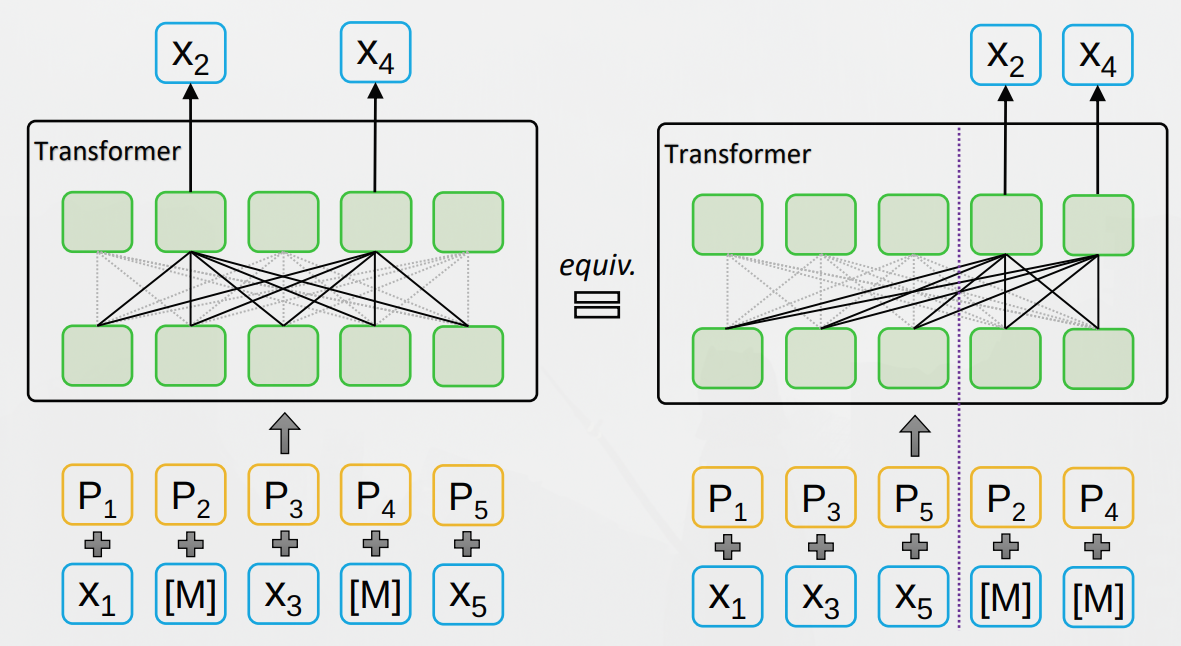
\includegraphics[width=\textwidth]{MPNetMLM.png}
        \caption{Masked language modelling (left) compared to the permuted order (right, unified view).}
        \label{fig:MPNetMLM}
    \end{subfigure}%
    \hfill
    \begin{subfigure}[b]{0.455\textwidth}
        \centering
        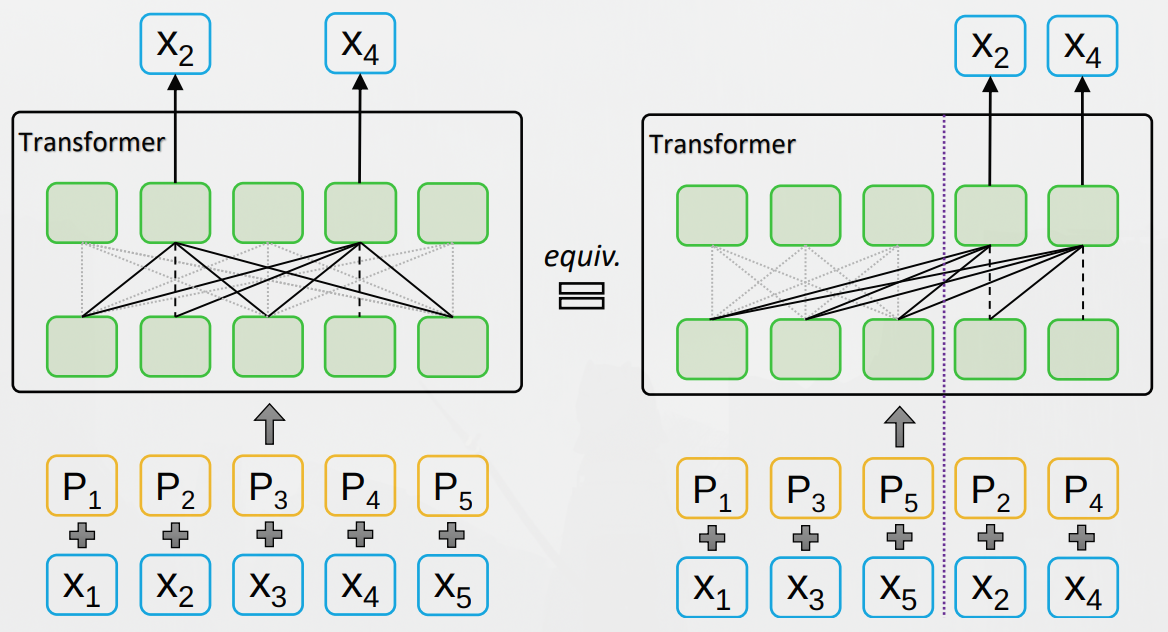
\includegraphics[width=\textwidth]{MPNetPLM.png}
        \caption{Permutation language modelling (left) compared to the permuted order (right, unified view).}
        \label{fig:MPNetPLM}
    \end{subfigure}
    \caption{Comparison of both masked and permutation language modelling pre-training objectives. Here, tokens are denoted $X_i$, masked tokens are denoted \texttt{[M]} and positional encoding is denoted $P_i$. Source: (\citet{song2020mpnet}).}
    \label{fig:mpnet}
\end{figure}


\subsubsection{Nomic}\label{sec:nomic}

The second model evaluated is Nomic. This model, released in 2024, represents a state-of-the-art, open-source text embedding model specifically designed for long-context understanding and reproducibility \cite{nussbaum2024nomic, nussbaum2024nomic1.5}. Version 1.5, used in this project, builds upon the initial release with features like Matryoshka Representation Learning (MRL) and multi-modal support.


The relevant adaptions and justifications are listed below.
\begin{itemize}
    \item Long context handling via RoPE - Nomic utilise Rotary Positional Embeddings (RoPE) instead of traditional positional embeddings \cite{su2024roformer, nussbaum2024nomic, vaswani2017attention}. RoPE encodes positional information using rotations, which has been shown to improve model generalisation to sequences of lengths not seen during pre-training (whether longer or shorter) \cite{su2024roformer}. This is a significant advantage for the Operalog dataset, where \texttt{FaultDescription} entries vary greatly in length (Figure~\ref{fig:hists}), helping ensure effective semantic understanding by the model.
    \item Computational efficiency - Despite its capabilities, Nomic v1.5 maintains a relatively small parameter count of around 137 million compared to other leading models, whose parameter counts typically exceed 1 billion significantly. It also incorporates architectural optimizations like FlashAttention \cite{dao2022flashattention}, an I/O-aware attention mechanism that reduces memory usage and latency during inference \cite{nussbaum2024nomic}. These factors were significant in selecting Nomic, as they allow the model to run efficiently within the constraints of the available 6GB GPU VRAM (Table~\ref{tab:researchHw}), unlike larger models such as Qwen2 or Mistral-7B (Table~\ref{tab:excludedModels}).
    \item Task-specific optimisation - Nomic supports task-specific prefixes prepended to the input text. For this project, the `clustering:' prefix was used for all \texttt{FaultDescription} entries fed into the Nomic model. This technique enables the model to produce embeddings specifically optimized for clustering tasks, by leveraging distinct semantic embedding subspaces learned during pre-training \cite{nussbaum2024nomic}. Utilising this prefix aims to enhance the quality of the embedding space specifically for the goal of grouping similar fault types, potentially leading to more coherent and meaningful clusters.
    \item Matryoshka Representation Learning (MRL) - Nomic version 1.5 incorporates MRL, which trains the model to produce nested embeddings where shorter prefixes of the full embedding vector still form meaningful representations \cite{kusupati2022matryoshka, nussbaum2024nomic1.5}. While the full 768-dimension embedding was used for this project, with MRL creating a structured embedding space, it opens up the possibility of detecting patterns that aid fault categorisation  more easily.
    \item Modern Architecture Choices - Nomic also incorporates other modern design choices adapted from BERT, such as removing the next sentence prediction pre-training objective, which simplifies pre-training and allowing for longer contiguous text processing, and using 0\% dropout, reflecting findings on training with very large datasets \cite{nussbaum2024nomic, liu2019roberta, xue2023repeat}. These contribute to its overall efficiency and performance.
    \item Benchmark Performance - Nomic version 1.5 demonstrates strong performance on the MTEB leaderboard, particularly for its size, ranking well on clustering tasks and providing empirical validation for its selection \cite{muennighoff2022mteb, nussbaum2024nomicelo}.
\end{itemize}

For further technical details on the Nomic architecture, pre-training and MRL, readers are referred to the relevant publications \cite{nussbaum2024nomic, nussbaum2024nomic1.5, kusupati2022matryoshka}.


\subsection {Section Summary}
MPNet and Nomic satisfied the criteria set out initially, including the hardware requirements and dataset features identified previously. They are therefore carried forward through the remaining portion of the pipeline. 

\section{Embedding dimensionality reduction}

% Motivated by the need for visualisation of the high-dimensional embedding space we explore dimensionality reduction techniques. Specifically we justify the applicability of two reduction techniques, Principal Component Analysis (PCA) \cite{pearson1901liii, hotelling1933analysis} and Uniform Manifold Approximation and Projection (UMAP) \cite{mcinnes2018umap}. Through justification from visualisation and literature, we decide to continue using UMAP in our pipeline. Apart from these two techniques, there was also consideration of t-distributed Stochastic Neighbour Embedding (t-SNE). However, as UMAP is known to be most consistent across runs and tends to better preserve the global structure of the data and due to the time constrained nature of this project, we opted to not explore t-SNE. Below, we show the justification in using UMAP for our dimensionality reduction use-case and explore the various hyperparameter applications to our dataset.

The high dimensionality (768 dimensions) of the text embeddings necessitates dimensionality reduction, initially to enable visualisation and subsequently to aid clustering (referring to the `curse of dimensionality' \cite{verleysen2005curse}, see Section~\ref{sec:dimred} for more details). This section explores and justifies the applicability of two techniques for this purpose: Principal Component Analysis (PCA) \cite{pearson1901liii, hotelling1933analysis}, a linear method, and Uniform Manifold Approximation and Projection (UMAP) \cite{mcinnes2018umap}, a non-linear manifold learning approach. While another non-linear technique, t-distributed Stochastic Neighbour Embedding (t-SNE), was initially considered, we focused on the evaluation of PCA and UMAP. This decision was based on UMAP's reported advantages in preserving global data structure more effectively than t-SNE, alongside its generally greater computational efficiency and run-to-run consistency \cite{mcinnes2018umap}. Given the project's scope, these practical benefits drew us away from t-SNE. The following subsections present a comparison between PCA and UMAP based on visualisations, justify the subsequent selection of UMAP for our pipeline; and detail its hyperparameter application to the Operalog dataset.

\subsection{Visualisation}

An example visualisation comparing the 3-dimensional projection, obtained using both PCA and UMAP in both MPNet and Nomic embedding spaces, is shown in Figure~\ref{fig:dimred-compare}. Since the original data resides in a 768-dimension embedding space, direct visualisation is impossible. Projecting this data down to the three dimensions enables visualisation but potentially loses information, making purely visual comparisons between the method outputs subjective.

To supplement the visual assessment with a quantitative measure, we evaluate the spread within these 3-dimensional projections using normalised variance. Normalised variance, defined for a data matrix $X$ in Equation~\ref{eq:normvar}, serves as a metric to quantify the overall dispersion of the points in the low-dimensional space.
Observing Figure~\ref{fig:dimred-compare}, the UMAP projections visually appear to exhibit more defined structures, such as clearer separations and groupings of points. Comparatively, the corresponding PCA projections look more dispersed and do not show any `clusters' or groupings of points. This visual impression is supported quantitatively by the normalised variance metric, calculated for these specific runs. The values for the UMAP projections ($0.90$ for MPNet, $2.27$ for Nomic) are substantially lower and closer to 1 than those for PCA (approximately $1.0 \times 10^7$ for MPNet, $-2.4 \times 10^9$ for Nomic). In this context, the lower normalised variance for UMAP suggests a projection that arranges the data more compactly while potentially preserving meaningful neighbourhood relationships, consistent with UMAP's goal of modelling the data manifold.

\begin{align}
    \text{Normalised Variance}(X) = \frac{\text{Var}(X)}{\text{Mean}(X)}
    \label{eq:normvar}
\end{align}

However, as discussed in Section~\ref{sec:umap}, UMAP is a stochastic algorithm. That is, due to an element of algorithmic randomness, its output naturally varies between runs \cite{mcinnes2018umap}. To account for this variability, Figure~\ref{fig:normvarumap} visualises the distribution of normalised variance results obtained over 100 independent UMAP runs for both embedding spaces. While variation exists, these distributions reaffirm the concept that UMAP consistently produces projections with significantly lower normalised variance than those produced by PCA. The distributions exhibit some right-skewness, particularly for the MPNet embeddings but remain concentrated in a range indicative of more structured projections than those from PCA.

Based on the combination of visually apparent characteristics in the example projections Figure~\ref{fig:dimred-compare} and the consistently lower (although variable) normalised variance scores, indicative of the better preservation of manifold structure, in Figure~\ref{fig:normvarumap}, UMAP is selected as the dimensionality reduction technique for the remainder of this pipeline. It appears more likely, than PCA, to produce a low-dimensional representation that retains structural information beneficial for the next clustering stage. 



\begin{figure}[htbp]
\centering
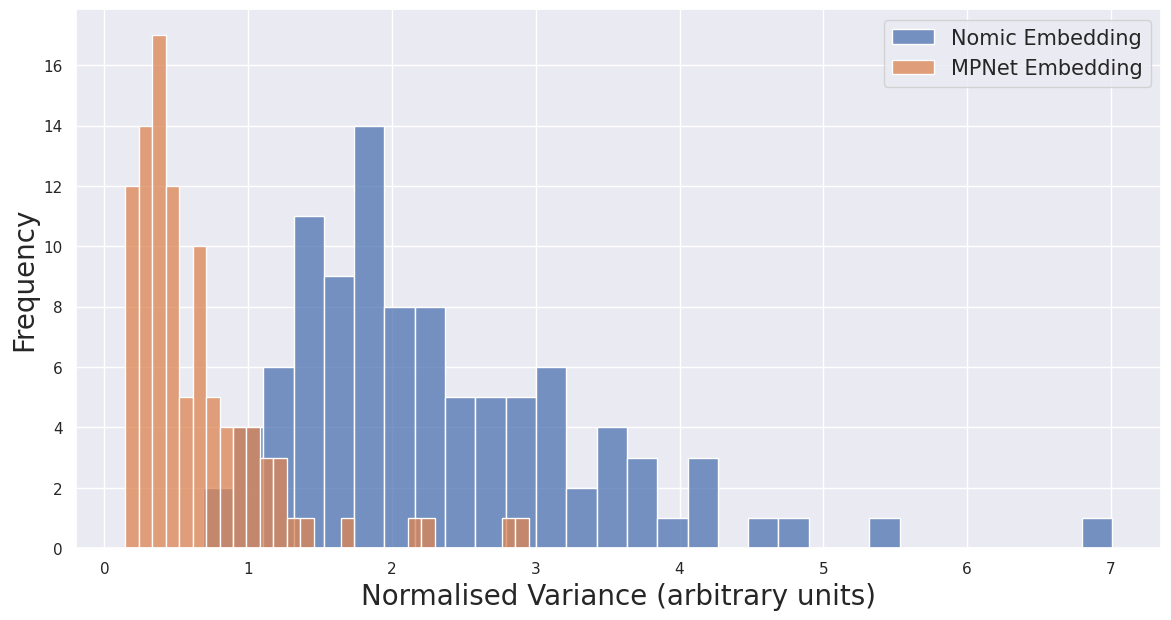
\includegraphics[width=0.8\textwidth]{distUMAP.png}
\caption{Histogram plot of 100 UMAP runs' normalised variance (Equation~\ref{eq:normvar}) is shown for both MPNet and Nomic embedding spaces of the Operalog \texttt{FaultDescription} entries. UMAP parameters: \texttt{min\_dist} $=0.1$, \texttt{n\_neighbors} $=15$, \texttt{metric} $= \text{cosine}$.}
\label{fig:normvarumap}
\end{figure}
\begin{figure}[htbp]
  \centering
  % Row 1: MPNet
  \begin{subfigure}[b]{0.48\textwidth}
    \centering
    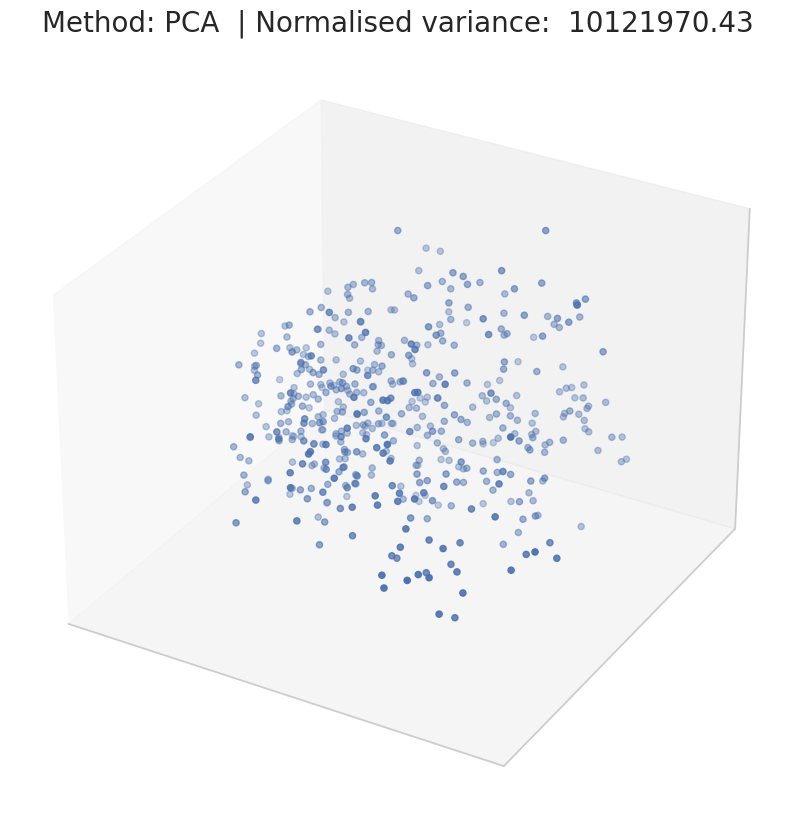
\includegraphics[width=\textwidth]{pcaTestMPNet.png}
    \caption{MPNet --- PCA}
    \label{fig:pcaTest-mpnet}
  \end{subfigure}%
  \hfill
  \begin{subfigure}[b]{0.48\textwidth}
    \centering
    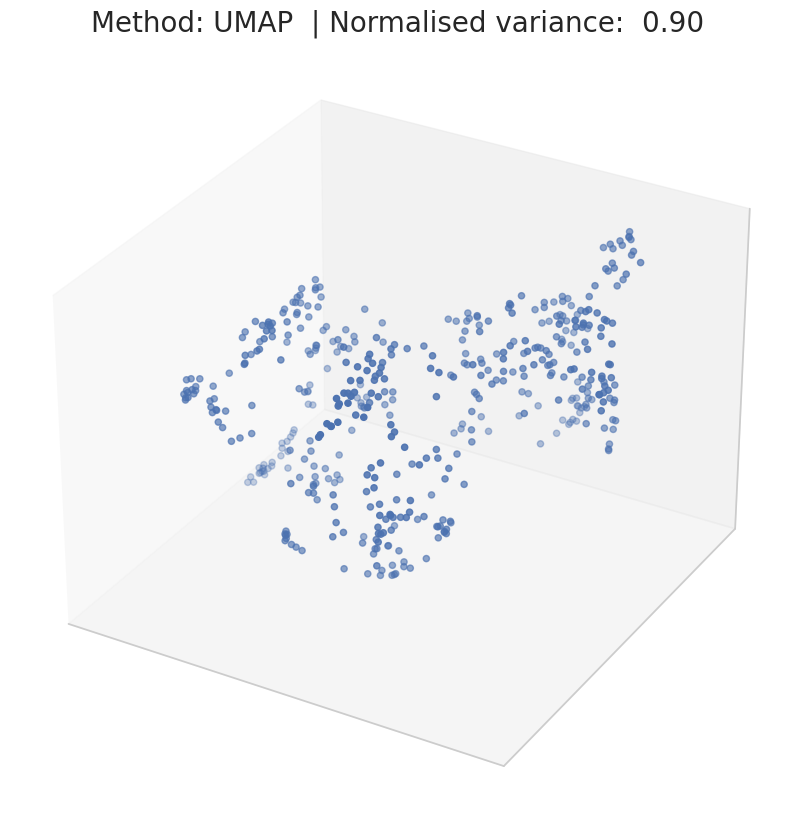
\includegraphics[width=\textwidth]{umapTestMPNet.png}
    \caption{MPNet --- UMAP}
    \label{fig:umapTest-mpnet}
  \end{subfigure}
  \vspace{1em} % space between rows
  % Row 2: Nomic
  \begin{subfigure}[b]{0.48\textwidth}
    \centering
    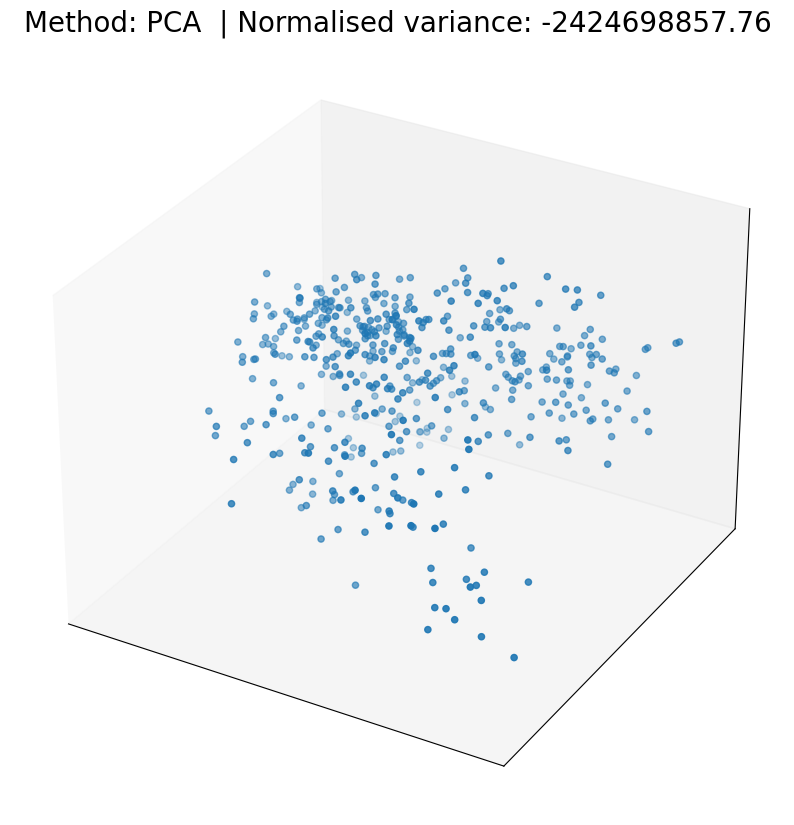
\includegraphics[width=\textwidth]{pcaTestNomic.png}
    \caption{Nomic --- PCA}
    \label{fig:pcaTest-nomic}
  \end{subfigure}%
  \hfill
  \begin{subfigure}[b]{0.48\textwidth}
    \centering
    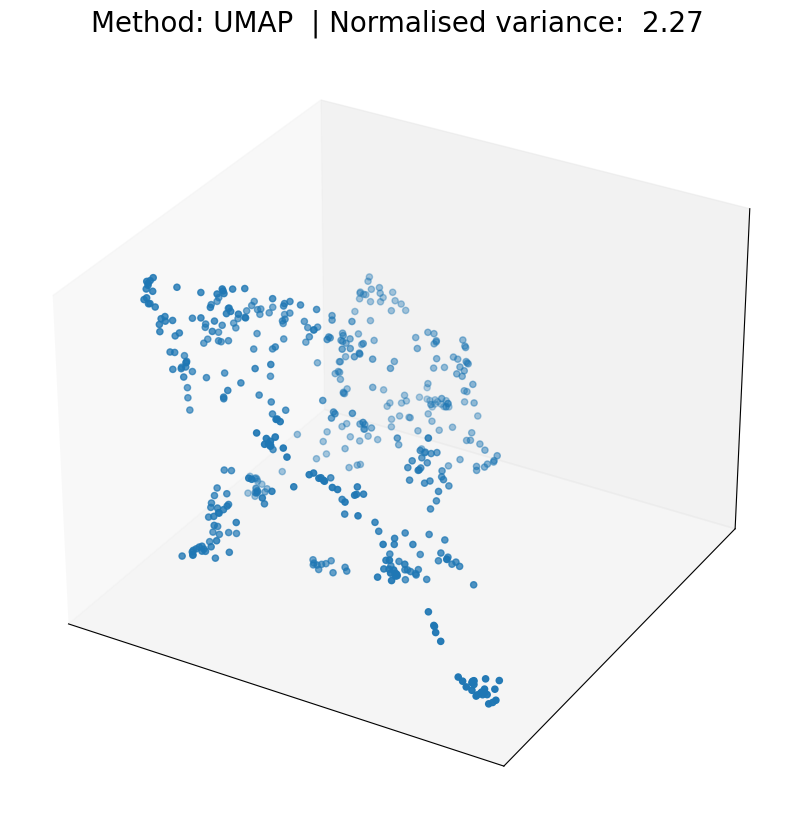
\includegraphics[width=\textwidth]{umapTestNomic.png}
    \caption{Nomic --- UMAP}
    \label{fig:umapTest-nomic}
  \end{subfigure}
  \caption{Comparison of PCA versus UMAP dimensionality reduction on the MPNet (top row) and Nomic (bottom row) embedding spaces on Operalog \texttt{FaultDescription} entries Normalised variance (Equation~\ref{eq:normvar}) is shown. UMAP parameters: \texttt{min\_dist} $=0.1$, \texttt{n\_neighbors} $=15$, \texttt{metric} $= \text{cosine}$.}
  \label{fig:dimred-compare}
\end{figure}

% \todo[inline, caption={}] {
%     \begin{itemize}
%         \item Talk about the visualisation mpnet vs nomic
%         \item {Talk about all the hyperparameters of the library, and add all the images generated for nomic and mpnet to the appendix. highlight that this not the end, right now we have no quantitative measure of deciding what is correct and what is not. So look forward to the clustering and hyperparameter section.}
%     \end{itemize}
% }

\subsection{UMAP Hyperparameters}

% As mentioned in Section~\ref{sec:umap}, UMAP has 4 main hyperparameters, described below. Evidently, from the previous section, it is unintuitive to decide which embedding space is `better' or even what values to set the model parameters. 
%
% Here we touch on how the parameters may affect the Operalog data.
%
% \todo[inline, caption={}] {
%     \begin{itemize}
%         \item justify the tuning 
%         \item introduce the experimentation
%         \item connect main text to appendix
%         \item summarise findings / selection
%         % \item Talk about how each hyperparameter works, and what we did to tune this.
%         % \item Talk about how they affect.
%     \end{itemize}
% }


As discussed in Section~\ref{sec:umap}, % Adjust reference to where UMAP is introduced
tuning UMAP's hyperparameters is crucial for obtaining a meaningful low-dimensional representation of the high-dimensional Operalog text embeddings. The choice of parameters like \texttt{n\_neighbors} and \texttt{min\_dist}, along with the distance \texttt{metric}, significantly influences the resulting structure.

Based on the nature of the Operalog data, adjusting \texttt{n\_neighbors} involves a trade-off. Lower values might isolate highly specific or rare fault types but could cause fragmentation of broader categories. Higher values might group related issues more globally but risk merging unique sub-types. Given the mix of common and rare faults, exploring a range of neighbour values is necessary. 

Similarly, \texttt{min\_dist} affects the visual density. Here, lower values may create tightly packed, visually distinct clusters suitable for identifying major categories. However, higher values might reveal finer intra-cluster variations relevant for understanding subtypes, but could make overall separation less clear. This parameter will affect clustering algorithms, such as DBSCAN as it essentially determines potential cluster density \cite{ester1996density}.
% [*Optional: Add a sentence about the potential impact on density-based clustering if applicable.*]
The choice of \texttt{metric} (i.e. `cosine' vs. `euclidean') is also critical, as `cosine' is often better suited for high-dimensional text embeddings like those used here \cite{baba2017plagiarism, cao2024recent}.

To gain an initial understanding of suitable UMAP parameters for the Operalog data, a naive grid search was performed using both MPNet and Nomic embeddings across the parameter ranges displayed in Table~\ref{tab:umapgrid}. The resulting visualisations for each parameter combination are presented in Appendix~\ref{app:umaphypgrid}. However, visual inspection of these results highlighted a surprising finding: contrary to common practice for text embeddings, cosine distance did not appear to yield projections demonstrably better at preserving structure more faithfully than Euclidean distance in this preliminary exploration. These inconclusive and unexpected outcomes underscore the need for a more systematic hyperparameter optimisation phase, which is later detailed in Section~\ref{sec:hyperparameterOpt}.

\begin{table}[htbp]
    \fontsize{8}{11}\selectfont % Kept your font size setting
    \centering
    \caption{UMAP hyperparameter values explored in naive grid search} % Correct caption
    \label{tab:umapgrid} % Kept your label
    \renewcommand{\arraystretch}{1.2} % Increase vertical spacing between rows slightly
    \rowcolors{2}{gray!10}{white} % Keep your row coloring
    \begin{tabular}{p{3cm}|p{8.5cm}} % Use left-aligned columns, no vertical rule
        \toprule % Top rule from booktabs
        \textbf{Hyperparameter} & \textbf{Values Explored} \\ % Column headers
        \midrule % Middle rule from booktabs
        \texttt{n\_neighbors} & $\big\{$ 5, 10, 13, 15, 20, 25 $\big\}$ \\ % Plain text list
        \texttt{min\_dist}    & $\big\{$ 0.0125, 0.05, 0.1, 0.15, 0.2 $\big\}$\\ % Plain text list
        \texttt{metric}       & $\big\{$ \texttt{'euclidean'}, \texttt{'cosine'} $\big\}$\\ % Keep texttt for strings
        \bottomrule % Bottom rule from booktabs
    \end{tabular}
    \renewcommand{\arraystretch}{1.0} % Reset arraystretch to default
\end{table}


% To empirically determine suitable parameters for the Operalog data using both MPNet and Nomic embeddings, a grid search was performed across a range of values for \texttt{n\_neighbors} and \texttt{min\_dist}, using the
% [State the metric you used, e.g., 'cosine'] distance metric and projecting to [State dimensions, e.g., 3] dimensions. The resulting visualisations for each combination are presented in [Reference Appendix and Figures, e.g., Appendix~B, Figures~B.1 through B.12].

% Visual inspection of these results
% [Reference Appendix again, e.g., in Appendix~B]
% revealed that
% [Summarise key observations from your 12 plots. E.g., "lower values of n\_neighbors (<10) tended to produce fragmented structures, while values above 50 overly smoothed distinct groups. A min\_dist below 0.1 created overly dense clusters where internal structure was lost, whereas values above 0.5 made separation difficult. The Nomic embeddings generally showed clearer structure across parameters compared to MPNet." - **REPLACE THIS WITH YOUR ACTUAL OBSERVATIONS**].

% Based on this analysis, the UMAP parameter configuration selected for subsequent clustering analysis (Section~\ref{sec:clustering_methods}) % Adjust reference if needed
% was \texttt{n\_neighbors=[Your chosen value]}, \texttt{min\_dist=[Your chosen value]}, and \texttt{metric='[Your chosen metric]'}. This configuration was chosen because it appeared to offer [State your justification based on observations. E.g., "the most informative balance between preserving local cluster separation (identifying distinct fault types) and representing the broader relationships between fault categories for both embedding models, based on the visual evidence in the appendix." - **REPLACE THIS WITH YOUR SPECIFIC JUSTIFICATION**].


\subsection{Section Summary}

Based on the comparison in the previous subsections, UMAP was selected over PCA as the preferred dimensionality reduction technique for the MPNet and Nomic embedding spaces. The preliminary visualisations also highlighted that UMAP's output is sensitive to its hyperparameters, indicating that a systematic approach is required to find optimal settings for revealing structure within the Operalog data. Directly evaluating the 'quality' of different UMAP projections is challenging therefore, to assess the effectiveness of various projections (resulting from different hyperparameter settings), we adopt an indirect evaluation strategy by applying clustering algorithms to the low-dimensional UMAP outputs. The quality of the resulting clusters, measured using specific clustering evaluation metrics (introduced in Section~\ref{sec:clusteringEval}), will serve as a proxy for how well the UMAP projection preserved the relevant structure for categorization. The next section introduces the clustering algorithms and metrics chosen for this purpose

% \todo[inline, caption={}]{
%     \begin{itemize}
%         \item motivate this with the curse of dimensionality and state the embedding spaces of the models - DONE
%         \item Here, we put some effort into visualisation of the embedding dimension with MPNET and with Nomic. Show images - DONE
%         \item Note that only unique sentences are considered for embedding (we have a one to one mapping backwards anyways). - DONE
%         \item In literature, there exists PCA and t-SNE and UMAP. Explain why we did not choose t-SNE and stuck with comparing UMAP and PCA. - DONE
%         \item Reason why UMAP is fine to use here, the topological manifold assumption (hard). - DONE
%         \item Talk about selecting UMAP and why over PCA. - DONE
%         \item Talk about UMAP parameters and how changing them affects things. - DONE
%         \item Talk about UMAP librarys and just lightly motivate this as an optimal  implementation. - SORT OF
%     \end{itemize}
% }

\section{Unsupervised categorisation through clustering}

The low-dimensional embedding space, projected by UMAP, is now ready for clustering. Clustering is the unsupervised machine learning task of grouping similar points together (see Section~\ref{sec:clustering}). Intuitively, each cluster produced by a clustering algorithm can be mapped uniquely to an Operalog fault category. However, as we are inducing fault categories `unsupervised', it is not immediate how to evaluate any one clustering. Three clustering algorithms were chosen, to compare against each other: k-Medoids \cite{kmedoids}, a partitioning-based clustering algorithm; DBSCAN \cite{ester1996density}, a density-based clustering algorithm; and HDBSCAN \cite{campello2013density}, a hybrid density and hierarchical clustering algorithm which is based on DBSCAN. In addition to this, k-Means \cite{macqueen1967some}, another partition-based clustering algorithm was considered but not chosen. This is due to the well-known disadvantages of k-Means; it is highly sensitive to the initialised configuration and it has issues with instability \cite{zhang2008improved}. This section outlines the clustering algorithms used and motivates the clustering heuristics used for clustering evaluation.

\todo{Maybe list these clustering heuristics explicitly here?}

\subsection{Clustering Candidates}

The k-Medoids clustering algorithm has one key hyperparameter (see Section~\ref{sec:kmedoids}), $k$, the number of initial clusters. Due to this, to select the optimal configuration, various values of $k$ must be tested against clustering heuristics. Additionally, as mentioned in the detailed description of the k-Medoids algorithm, the runtime complexity of the algorithm 

The DBSCAN algorithm has two key hyperparameters (see Section~\ref{sec:dbscan}), \texttt{Eps} and \texttt{MinPts}. 

The HDBSCAN algorithm only has one key hyperparameter (see Section~\ref{sec:hdbscan}), $m_{\text{pts}}$.

\todo{Heavily fix the wording here, discuss benefits and drawbacks of each for our operalog and motivate why we need to test all three.}

\subsection{Clustering heuristics}  

Motivated by the necessity to evaluate this open-ended problem, four clustering heuristics are utilised: inertia, ... \todo{list the others here}.


\todo[inline, caption={}]{
    \begin{itemize}
        \item mention k-medoids sklearn implementation uses PAM algorithm. Touch on the fact it only has one parameter, which is significant for our usecase
        \item motivate the clustering - DONE ISH
        \item talk about clustering algorithms we did not consider, with research - DONE ISh
        \item explain the 3 clustering methods we have chosen to use and the hyperparameters in a table
        \item show test clustering 
        \item this section is not really quantitative, highlight how we have to introduce clustering heuristics 
    \end{itemize}
}

\section{Hyperparameter optimisation}\label{sec:hyperparameterOpt}

\section{Label generation}

\section{CLI Application}\label{sec:CLI}

\todo[inline, caption={}]{
    \begin{itemize}
        \item Okay so we have done hyper parameter tuning etc but the real benefit of this tool is that it gives you a qualitatively assessable result in an easy to run format.
    \end{itemize}
}


\todo[inline,caption={}]{
    Describe the methods and procedures used.
    The things in this section will include.
    \begin{itemize}
        \item Explaining data format and data visualisation: wordcloud.
        \item Data cleaning steps, including removing key words such as Ion Source.
        \item Text preprocessing steps (cleaning) and computational challenges (tensorflow).
        \item Choosing the best sentence embedding transformer: MPNET, NOMIC.
        \item Data visualisation (before and after sentence embedding): similarity visualisation, explain unique sentences, token length distribution.
        \item Motivate why clustering in higher dimensions performs worse
        \item UMAP, PCA, t-SNE comparison. Motivate using UMAP.
        \item UMAP hyperparameter optimisation.
        \item Performing clustering with kmedoids, dbscan, hdbscan.
        \item Using optuna.
        \item Evaluation of results and choosing the best model (and arguing why hdbscan is the best by looking at the variance of dbscan and inflexibility of kmedoids)
        \item Touch on the production of a CLI application that allows you to mix and match various parts of the pipeline. Motivate the need for command line tool.
    \end{itemize}
}

\chapter{Results and Discussion}

\todo[inline,caption={}]{
Describe the results and analyse the results
\begin{itemize}
    \item Analyse the word cloud.
    \item Analyse the sentence embedding results.
    \item Analyse UMAP vs. PCA vs. t-SNE qualitatively and later quantitatively (compared to the clustering).
    \item Anaylse the UMAP hyperparameter optimisation qualitatively, mention that we use Optuna.

    \item Next steps: Fine tuning the PLM (Nomic or MPNet). Using MOE nomic (v2). Rent higher computation, then you can use top performing PLMS. Using t-SNE to see differences.
\end{itemize}
}

\chapter{Conclusion}

\todo[inline, caption={}]{
    \begin{itemize}
        \item Definitely talk about clear and transparent PLMs and malicious stuff (see BERT section).
    \end{itemize}
}

% \todo[inline,caption={}]{
% Summarize your findings and suggest areas for future work.
% }

% -------------------------
% References
% -------------------------
% \bibliographystyle{plainnat}

\bibliographystyle{plainnat}
\bibliography{refs}  % Uses the external file refs.bib

\appendix
\chapter{Further Discussion}
\section{MPNet Mathematical Formulations} \label{app:mpnet_maths}

This appendix provides supplementary mathematical details for the MPNet model discussed in Section~\ref{sec:rationalempnet}.

\subsection{MPNet Pre-training Objective}

The pre-training objective for MPNet aims to maximize the expected log-likelihood of predicting tokens based on a permuted context that includes information about masked tokens later in the sequence. Formally, let $\mathcal{Z}_{T}$ be the set of all $T!$ permutations of the index list $[1,...,T]$. For a given permutation $z=(z_{1},...,z_{T})$, let $x_{z_{i}}$ denote the token at original position $z_i$, and $x_{z<i}$ denote the sequence of tokens preceding $z_i$ in the permutation $z$. Let $M$ be the set of indices corresponding to masked tokens, and $M_{z>c}$ be the subset of masked token indices appearing after position $c$ in the permutation $z$. The objective is defined as \cite{song2020mpnet}:

\begin{equation} \label{eq:mpnet_objective_appendix}
\max_{\theta} \mathbb{E}_{z\in\mathcal{Z}_{T}} \left[ \sum_{i=1}^{T} \log p_{\theta}(x_{z_{i}} \mid x_{z<i}, M_{z>c}) \right]
\end{equation}

where $\theta$ represents the shared model parameters, fixed for each permutation $z$.


\subsection{MPNet Input Structuring Example}

To implement the objective (Equation~\ref{eq:mpnet_objective_appendix}), the input sequence is rearranged based on the permutation $z$ and a split point $c$. The sequence is divided into non-predicted tokens ($x_{z_{\le c}}$) and predicted tokens ($x_{z_{>c}}$). The input representation fed to the model concatenates the non-predicted part, mask token placeholders corresponding to the predicted part ($M_{z>c}$), and the actual predicted tokens (used only for loss calculation). For an example input sequence $(x_1, ..., x_6)$, a permutation $z=(x_3, x_5, x_2, x_1, x_4, x_6)$, and a split point $c=3$, the structured input is represented as \cite{song2020mpnet}:

\begin{equation} \label{eq:mpnet_input_appendix}
\langle x_{z_{\le c}}; M_{z>c}; x_{z_{>c}} \rangle = \langle x_3, x_5, x_2; [M], [M], [M]; x_1, x_4, x_6 \rangle
\end{equation}

where $[M]$ denotes the mask token placeholder.

% \subsection{MPNet Two-Stream Self-Attention Architecture}
%
% \begin{figure}[htbp]
%     \begin{center}
%         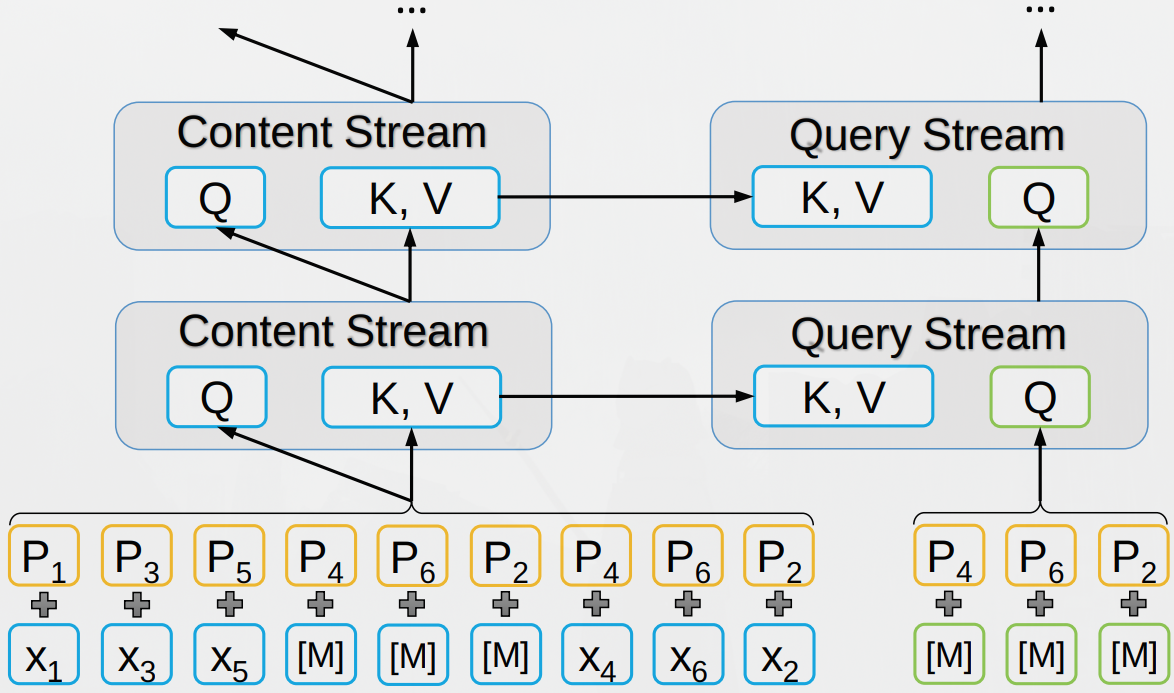
\includegraphics[width=0.5\textwidth]{MPNetTwoStreamSelfAttention.png}
%     \end{center}
%     \caption{The MPNet two-stream self-attention architecture illustration. Here, the query stream reuses the hidden value from the content stream for its key-value input. Source: (\citet{song2020mpnet})}\label{fig:MPNetTwoStreamSelfAttention}
% \end{figure}
% \begin{figure}[htbp]
%     \begin{center}
%         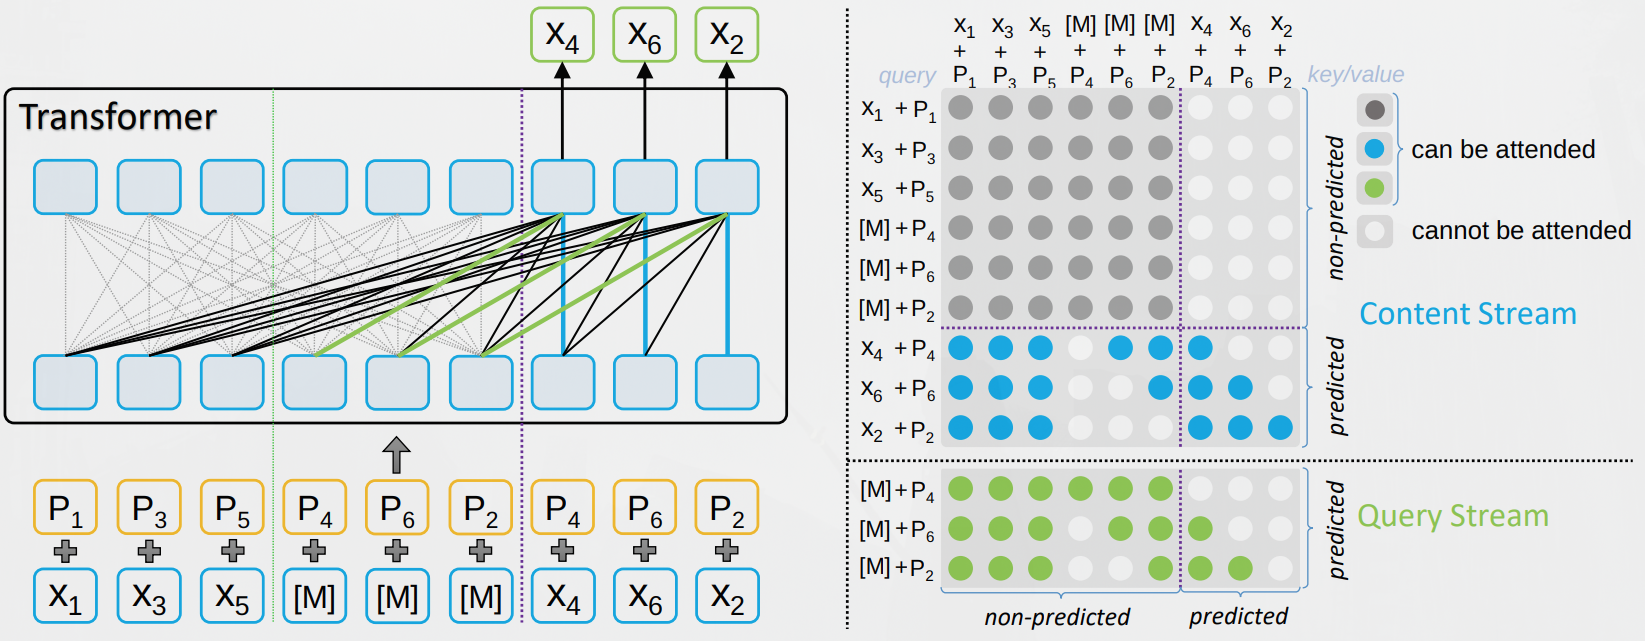
\includegraphics[width=0.95\textwidth]{MPNetTwoStreamSelfAttention1.png}
%     \end{center}
%     \caption{Illustration of the attention masks for an example input with 3 masked tokens. Left shows the transformer architecture with light grey attention masks Source: (\citet{song2020mpnet})}\label{fig:MPNetTwoStreamSelfAttention1}
% \end{figure}

% %It was shown in (\citet{song2020mpnet}) that under this unified view, masked language modelling and permutation language modelling both are able to represented in this unified view. As an illustration, take Figure~\ref{fig:mpnet} which shows how, for masked language modelling (Figure~\ref{fig:MPNetMLM}), it is equivalent first permute the input sequence and then mask a portion of the right-most tokens (both $x_2$ and $x_4$). Moreover, for permutation language modelling in Figure~\ref{fig:MPNetPLM} the input sequence is permuted, choosing the right most tokens as the predicted tokens \cite{song2020mpnet}. In either case, the tokens being predicted is the right of some index $c$ (the dotted line in the illustration). 
%
% % Formalising, let $\mathcal{Z_T}$ be some $T$-length set of all $T!$ permutations of the index list $[1,...,T]$. For a given permutation $z = (z_1, ..., z_T)$ we say $x_{(z_i)}$ denotes a token at position $z_i$ (and we denote $z_{<i}$ as all positions before some $1 \le i \le T$). Further, we let $M$ be a set of masked tokens, where $M_{z>c}$ denotes the masked tokens (\texttt{[M]} in Figure~\ref{fig:mpnet}) past the index $c$, mentioned before. Then, for some fixed model parameters $\theta$ we show the objective function in Equation~\ref{eq:mpnet} \cite{song2020mpnet}.
% %
% % \begin{align}
% %     \max_{\theta} \text{  } \mathbb{E}_{z\in\mathcal{Z}_T} \bigl[ \sum_{i=1}^{T} \log p_{\theta} \bigl(x_{z_i}\mid x_{z_{<i}}, M_{z_{>c}}\bigr) \bigr], \label{eq:mpnet}
% % \end{align}
%
% Formalising, let $\mathcal{Z}_T$ be the set of all $T!$ permutations of the
% index list $[1,\dots,T]$.  For a given permutation
% $z=(z_1,\dots,z_T)$ we denote $x_{(z_i)}$ the token at position $z_i$ and
% $z_{<i}$ the prefix positions.  Let $M$ be the set of masked tokens with
% $M_{z>c}$ the subset to the right of index $c$.
% The pre‑training objective is
% \begin{align}
%   \max_{\theta}\,
%   \mathbb{E}_{z\in\mathcal{Z}_T}
%   \Bigl[\sum_{i=1}^{T}\log p_{\theta}(x_{z_i}\mid x_{z_{<i}},M_{z_{>c}})\Bigr],
%   \label{eq:mpnet}
% \end{align}
% identical to Eq. (3) in \citet{song2020mpnet}.  
%
% % ➜  Suggestion: move the equation and derivation to Appendix A and leave a
% %    one‑line pointer here.
% To illustrate, a 6‑token input
% $(x_1,\dots,x_6)$ permuted as $(x_3,x_5,x_2,x_1,x_4,x_6)$ and masked after
% $c{=}3$ becomes
% $\langle x_3,x_5,x_2,[M],[M],[M],x_1,x_4,x_6\rangle$
% (see Fig.~\ref{fig:mpnet}).  % 🟥 6
% % ➜  Figure can stay if space allows; otherwise appendix.
%
% Clearly, this objective function looks very similar to that of the permutation language modelling. The main difference is the ability to capture the conditioning on the masked tokens, past some index $c$. To demonstrate this, take the following input 6 token input sequence $(x_1,x_2,...,x_6)$. After applying a random permutation, assume we have $(x_3, x_5, x_2, x_1, x_4, x_6)$ and are going to be masking 3 tokens (i.e. $c = 3$). A new input sequence is generated from concatenation of two parts: the non-predicted ($x_{z_{\le c}}$) and predicted ($x_{z_{>c}}$) parts. These parts are concatenated, joined with $M_{z_{>c}}$ masked tokens in between resulting in Equation~\ref{eq:concatmpnet} \cite{song2020mpnet}. \todo{Comment on this and what it basically means.}
% \begin{align}
%     \langle &x_{z_{\le c}}; M_{z_{>c}}; x_{z_{>c}} \rangle \\
%     = \langle &x_3, x_5, x_2, [M], [M], [M], x_1, x_4, x_6 \rangle
%     \label{eq:concatmpnet}
% \end{align}

\section{UMAP Hyperparameter Search} \label{app:umaphypgrid}

Figures~\ref{fig:mpnet1} through \ref{fig:nomic3} in this appendix illustrate the results of the naive grid search performed over the UMAP hyperparameters listed in Table~\ref{tab:umapgrid}, applied to both MPNet and Nomic embeddings of the Operalog \texttt{FaultDescription} entries. These visualisations demonstrate the effects of varying parameters like \texttt{n\_neighbors}, \texttt{min\_dist} and \texttt{metric} as described conceptually in Section~\ref{sec:umap}. Notably, visual inspection suggests that, for the goal of creating a low-dimensional representation that isolates structural groupings in this specific dataset, the `cosine' distance metric did not produce significantly different or clearly superior results compared to the `euclidean' metric. This outcome is somewhat surprising as cosine distance is frequently recommended for text embedding applications in the literature \cite{cao2024recent, baba2017plagiarism}. This observation, combined with the difficulty in determining the optimal settings purely through visual inspection of numerous plots, makes it evident that this naive grid search approach is insufficient. It therefore motivates the need for the systematic hyperparameter optimisation process detailed in Section~\ref{sec:hyperparameterOpt}.

\begin{figure}[htbp]
    \centering
    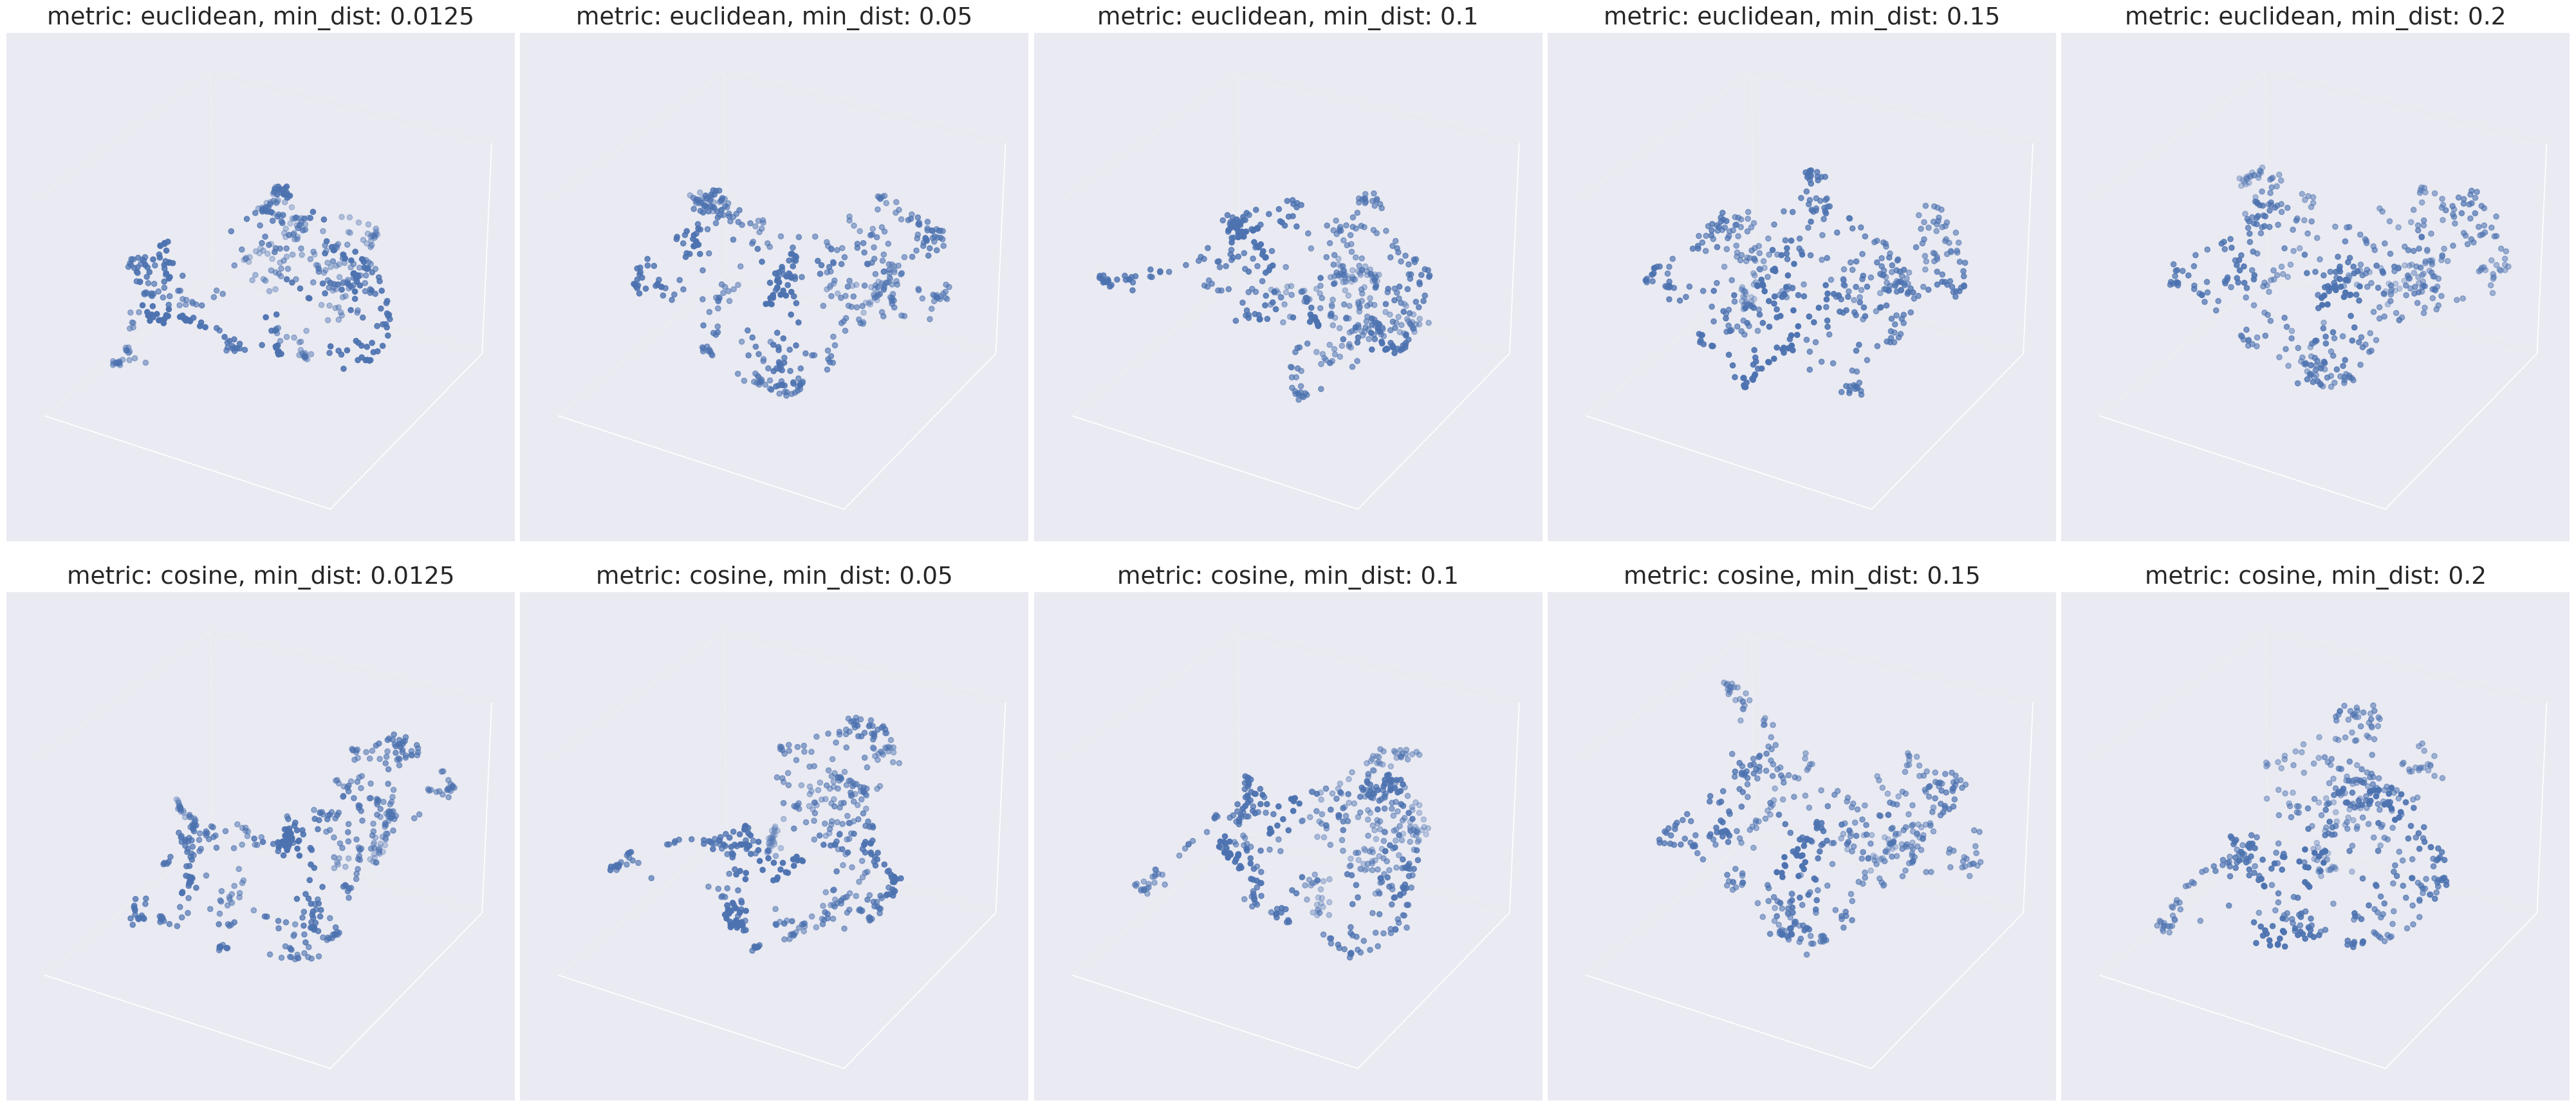
\includegraphics[width=\textwidth]{./images/mpnethyp1.png}
    \caption{MPNet, grid search for UMAP hyperparameter (see Table~\ref{tab:umapgrid}) over the parameters \texttt{metric} and \texttt{min\_dist}}
    \label{fig:mpnet1}
\end{figure}%
\begin{figure}[htbp]
    \centering
    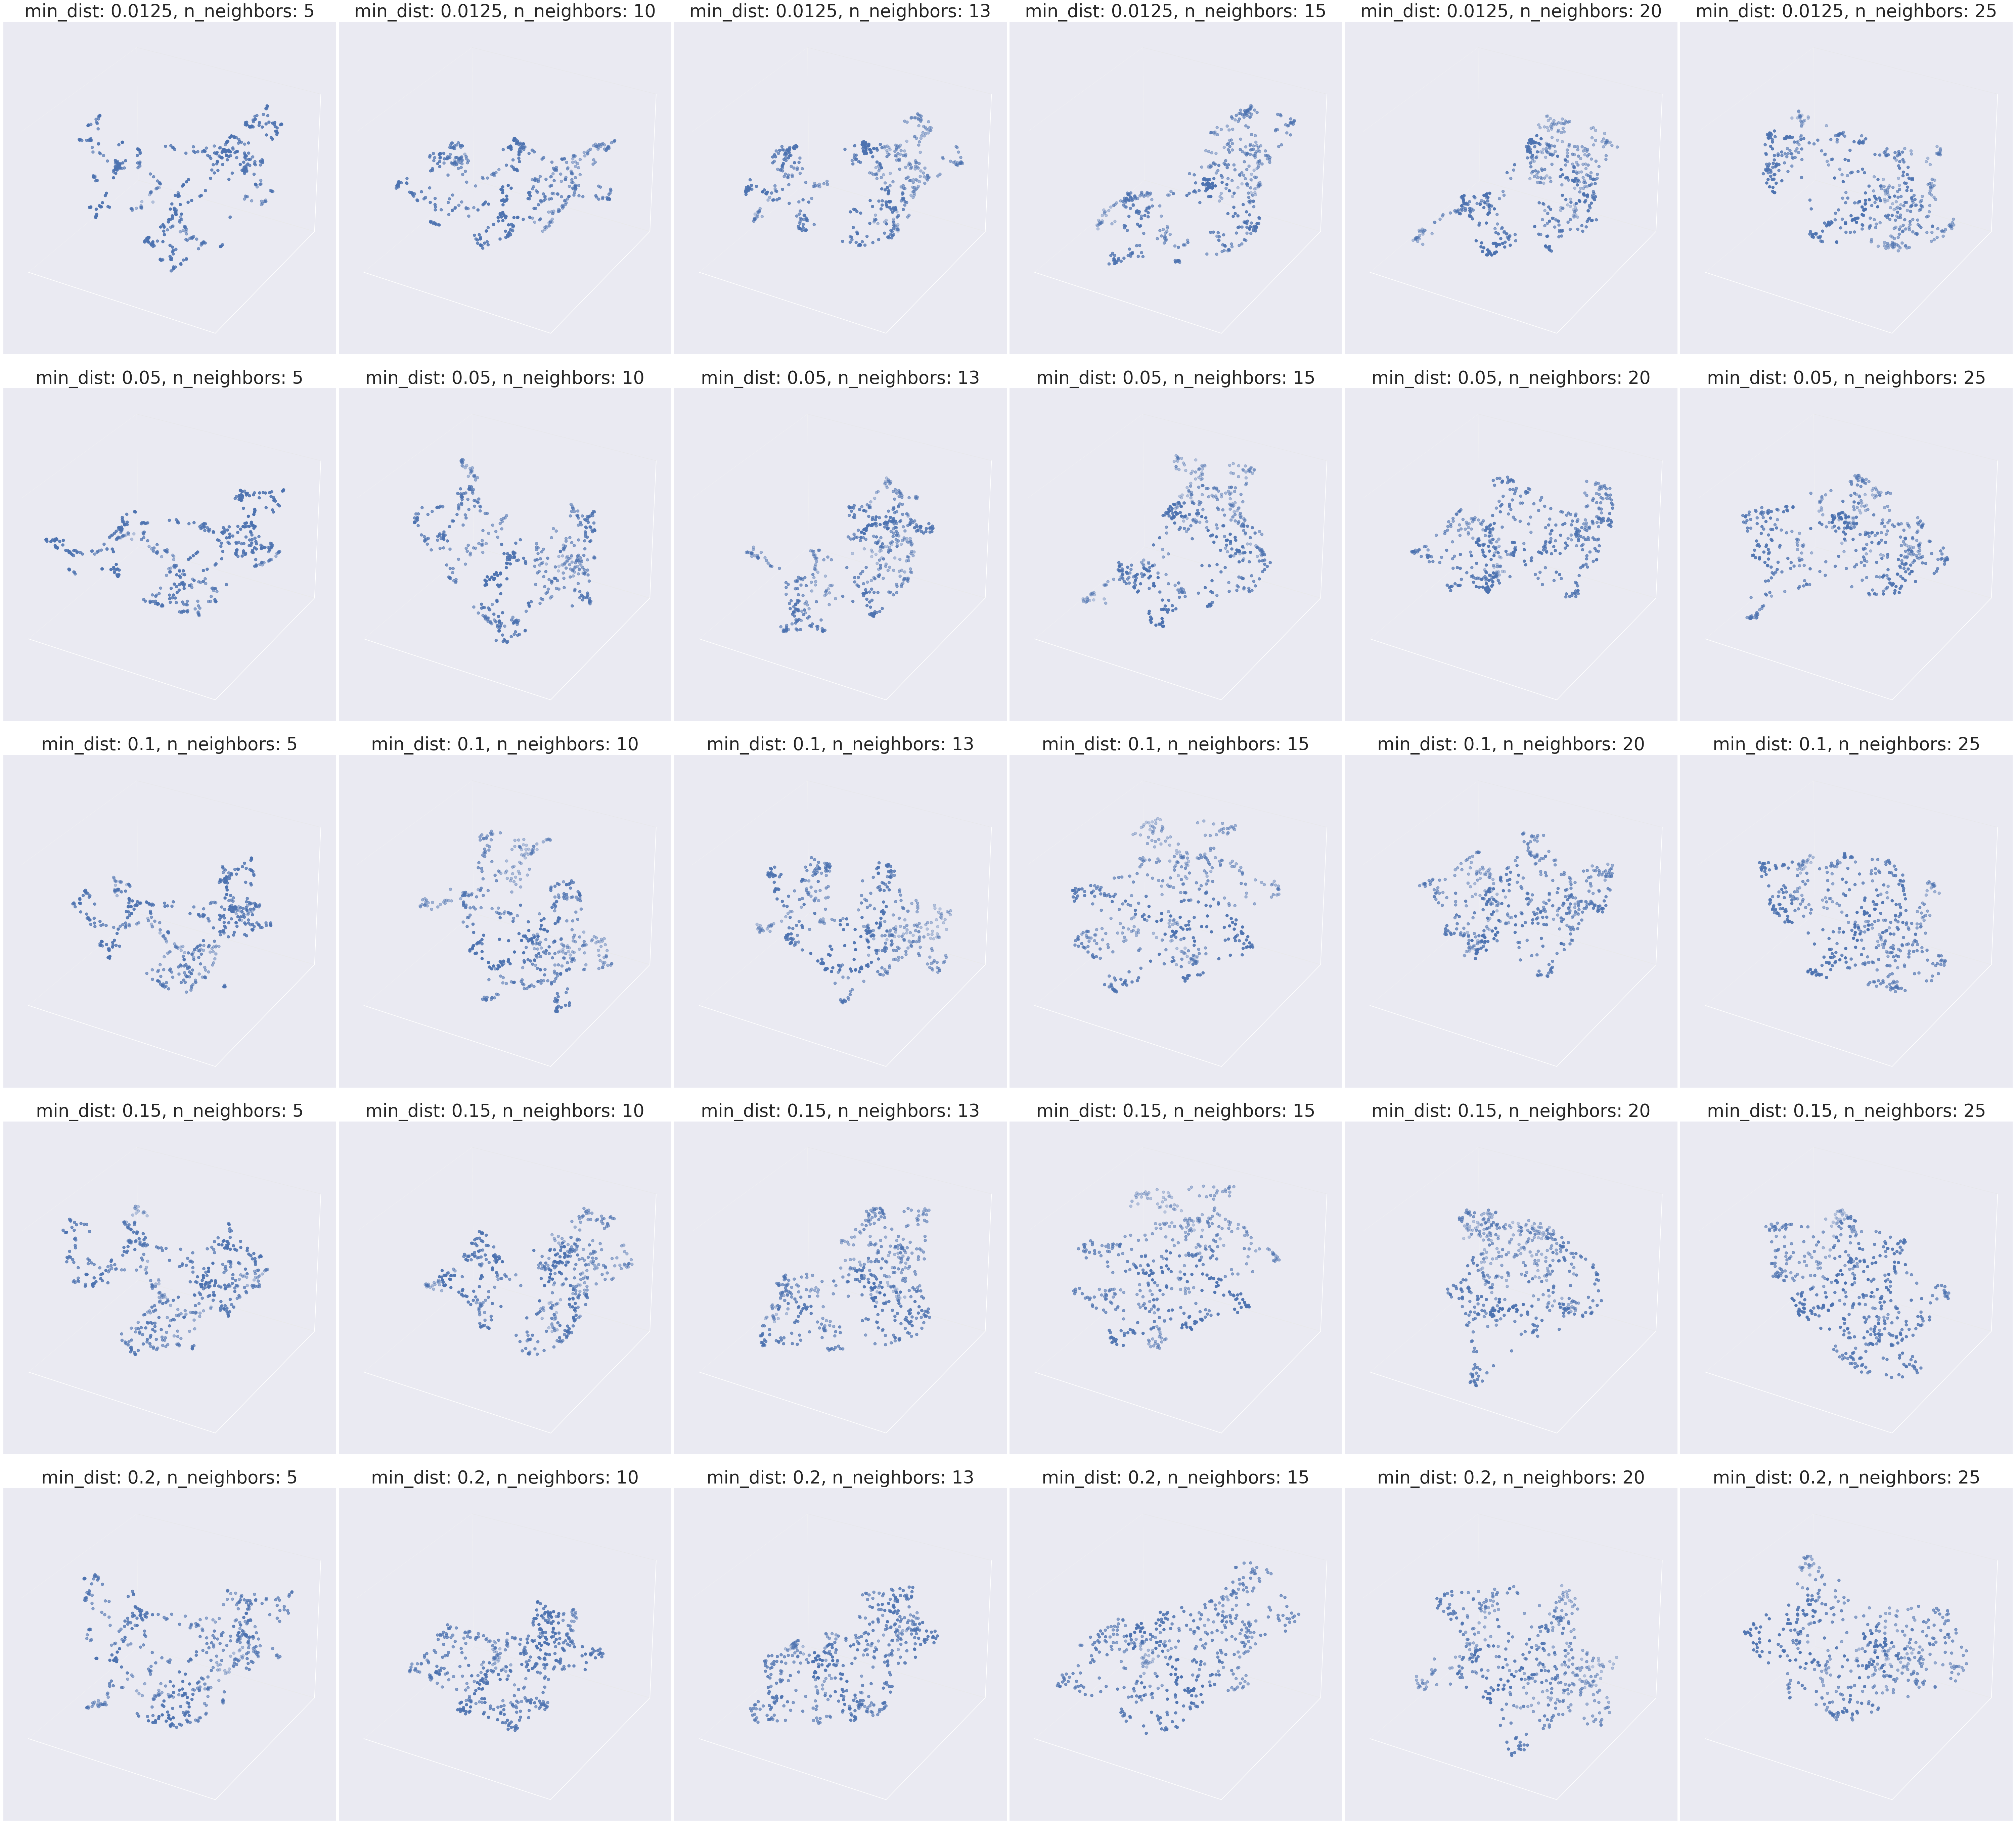
\includegraphics[width=\textwidth]{./images/mpnethyp2.png}
    \caption{MPNet, grid search for UMAP hyperparameter (see Table~\ref{tab:umapgrid}) over the parameters \texttt{min\_dist} and \texttt{n\_neighbors}}
    \label{fig:mpnet2}
\end{figure}%
\begin{figure}[htbp]
    \centering
    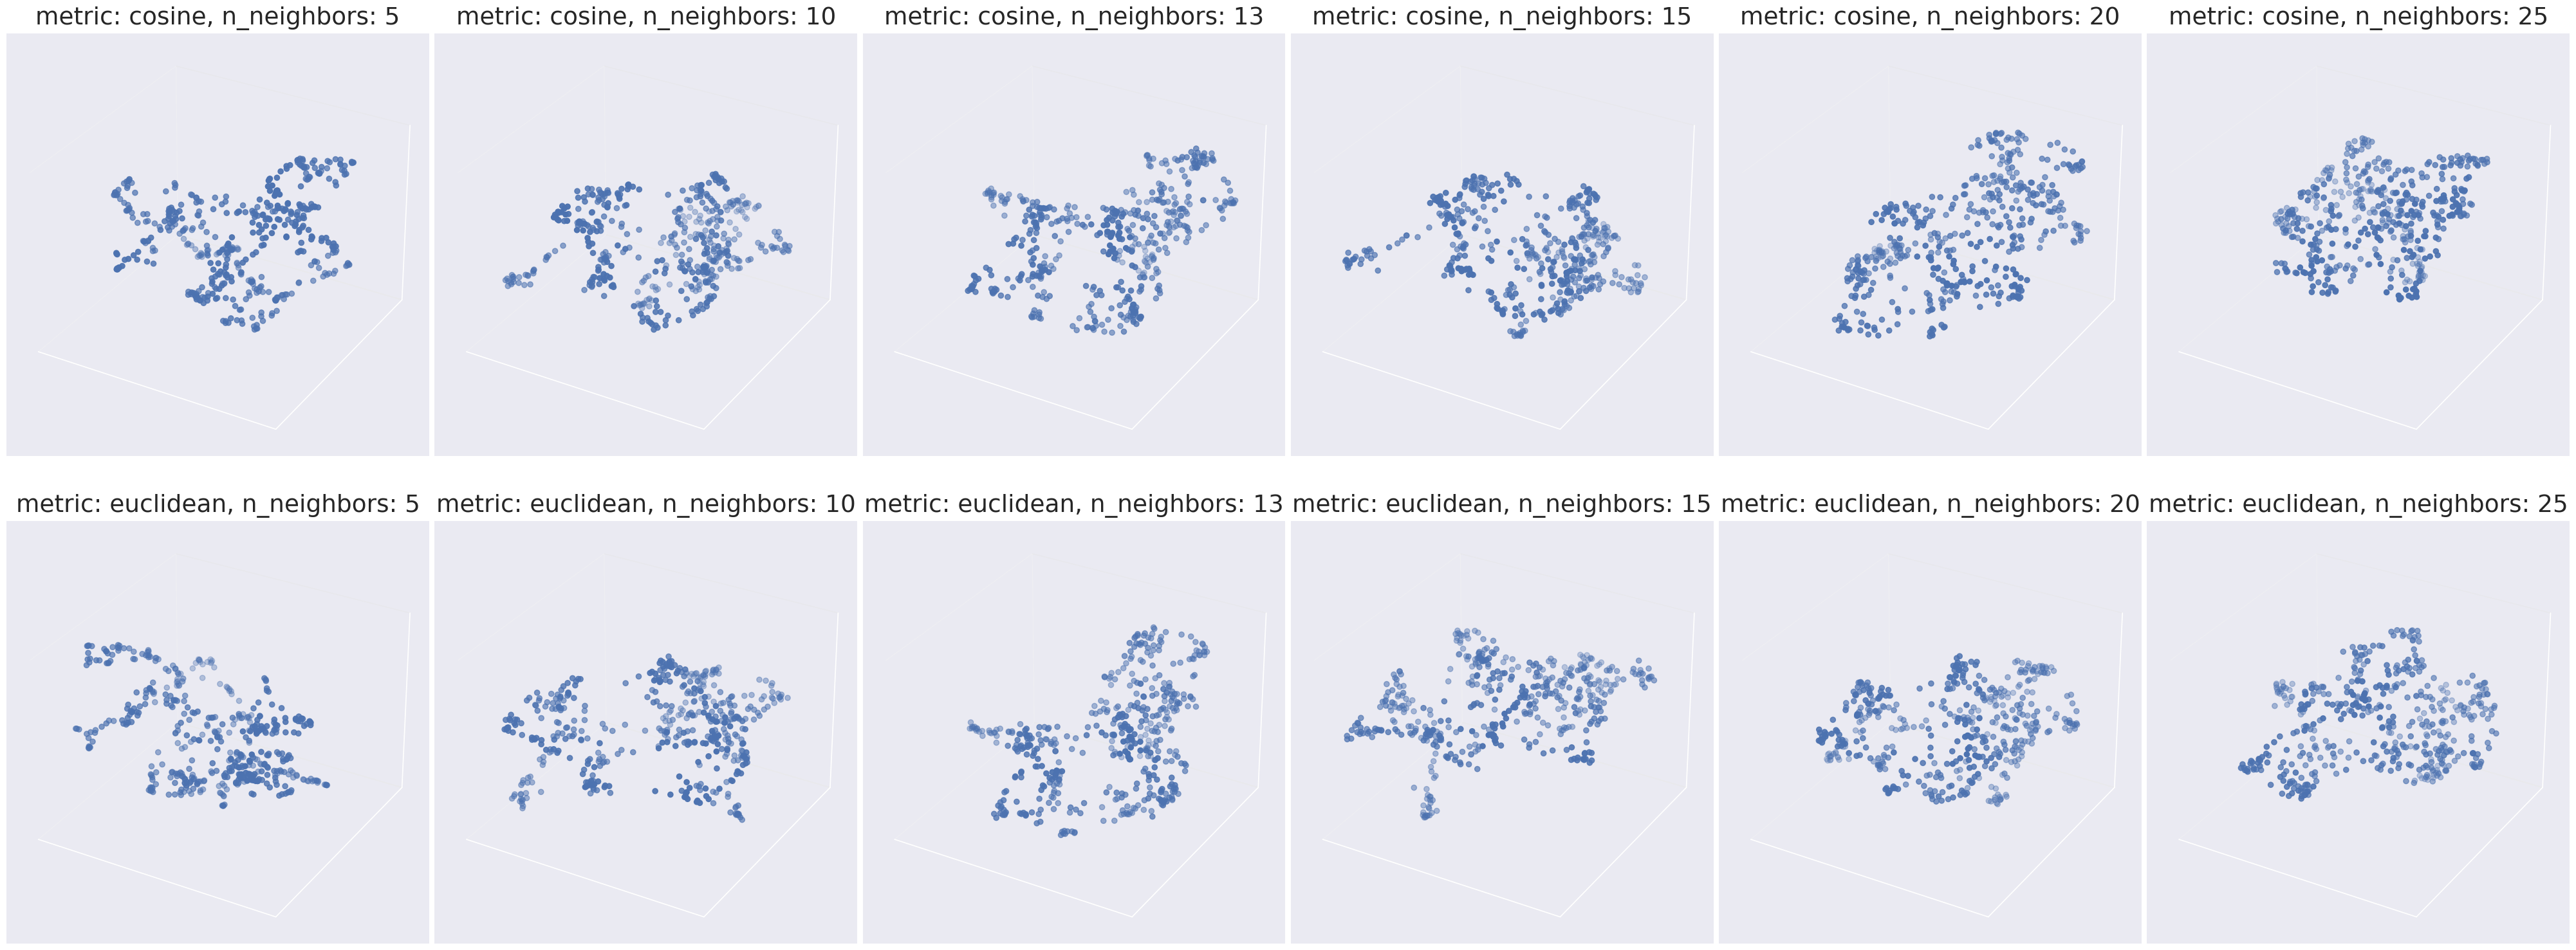
\includegraphics[width=\textwidth]{./images/mpnethyp3.png}
    \caption{MPNet, grid search for UMAP hyperparameter (see Table~\ref{tab:umapgrid}) over the parameters \texttt{metric} and \texttt{n\_neighbors}}
    \label{fig:mpnet3}
\end{figure}%
\begin{figure}[htbp]
    \centering
    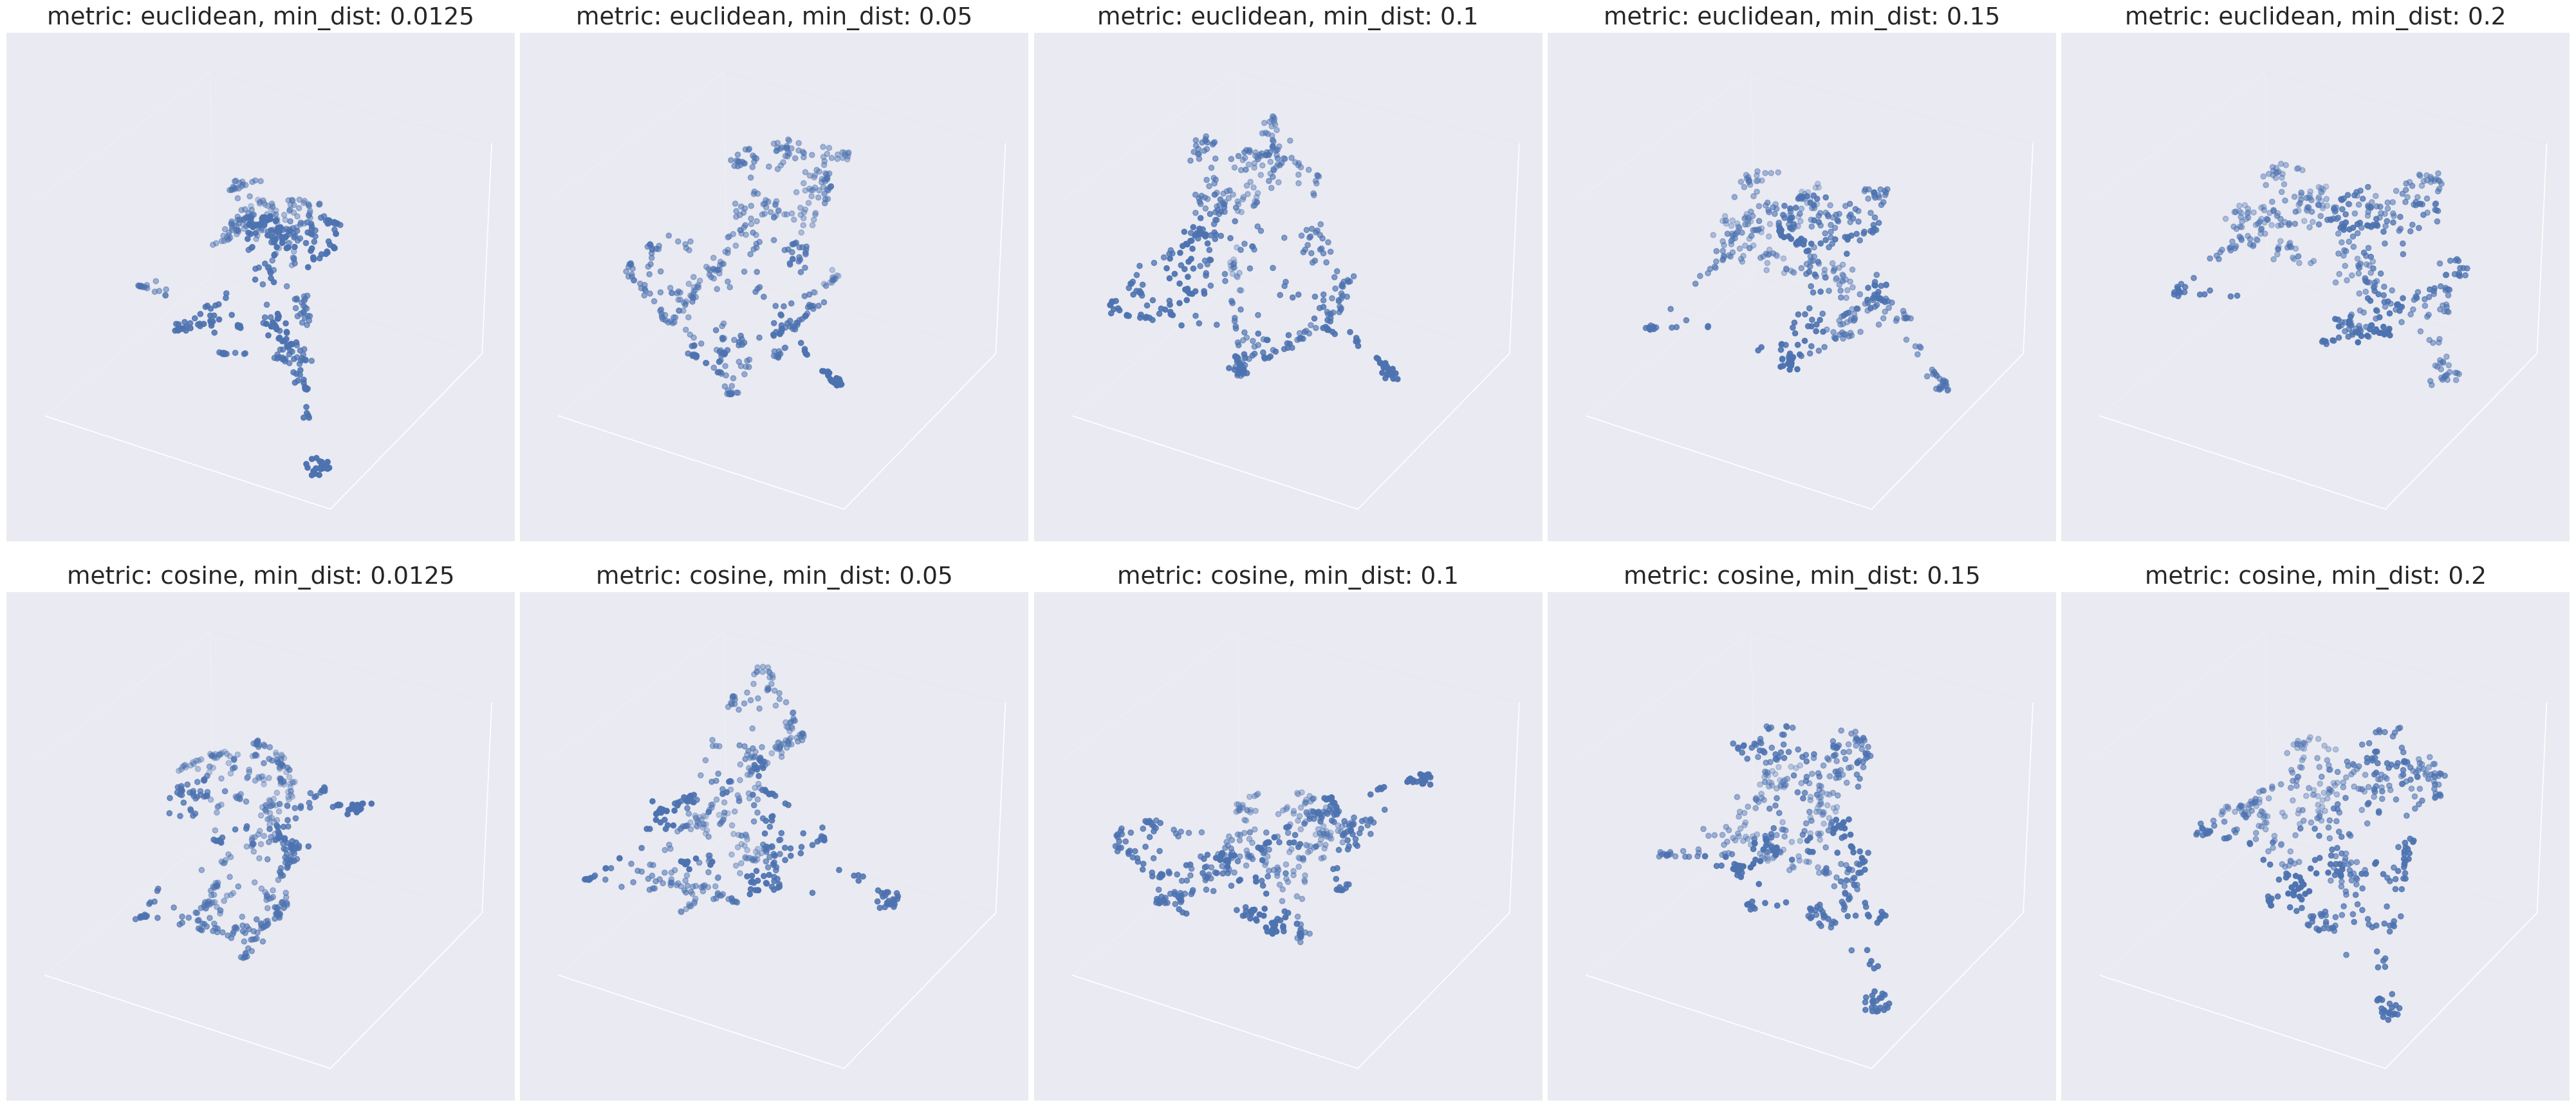
\includegraphics[width=\textwidth]{./images/nomichyp1.png}
    \caption{Nomic, grid search for UMAP hyperparameter (see Table~\ref{tab:umapgrid}) over the parameters \texttt{metric} and \texttt{min\_dist}}
    \label{fig:nomic1}
\end{figure}%
\begin{figure}[htbp]
    \centering
    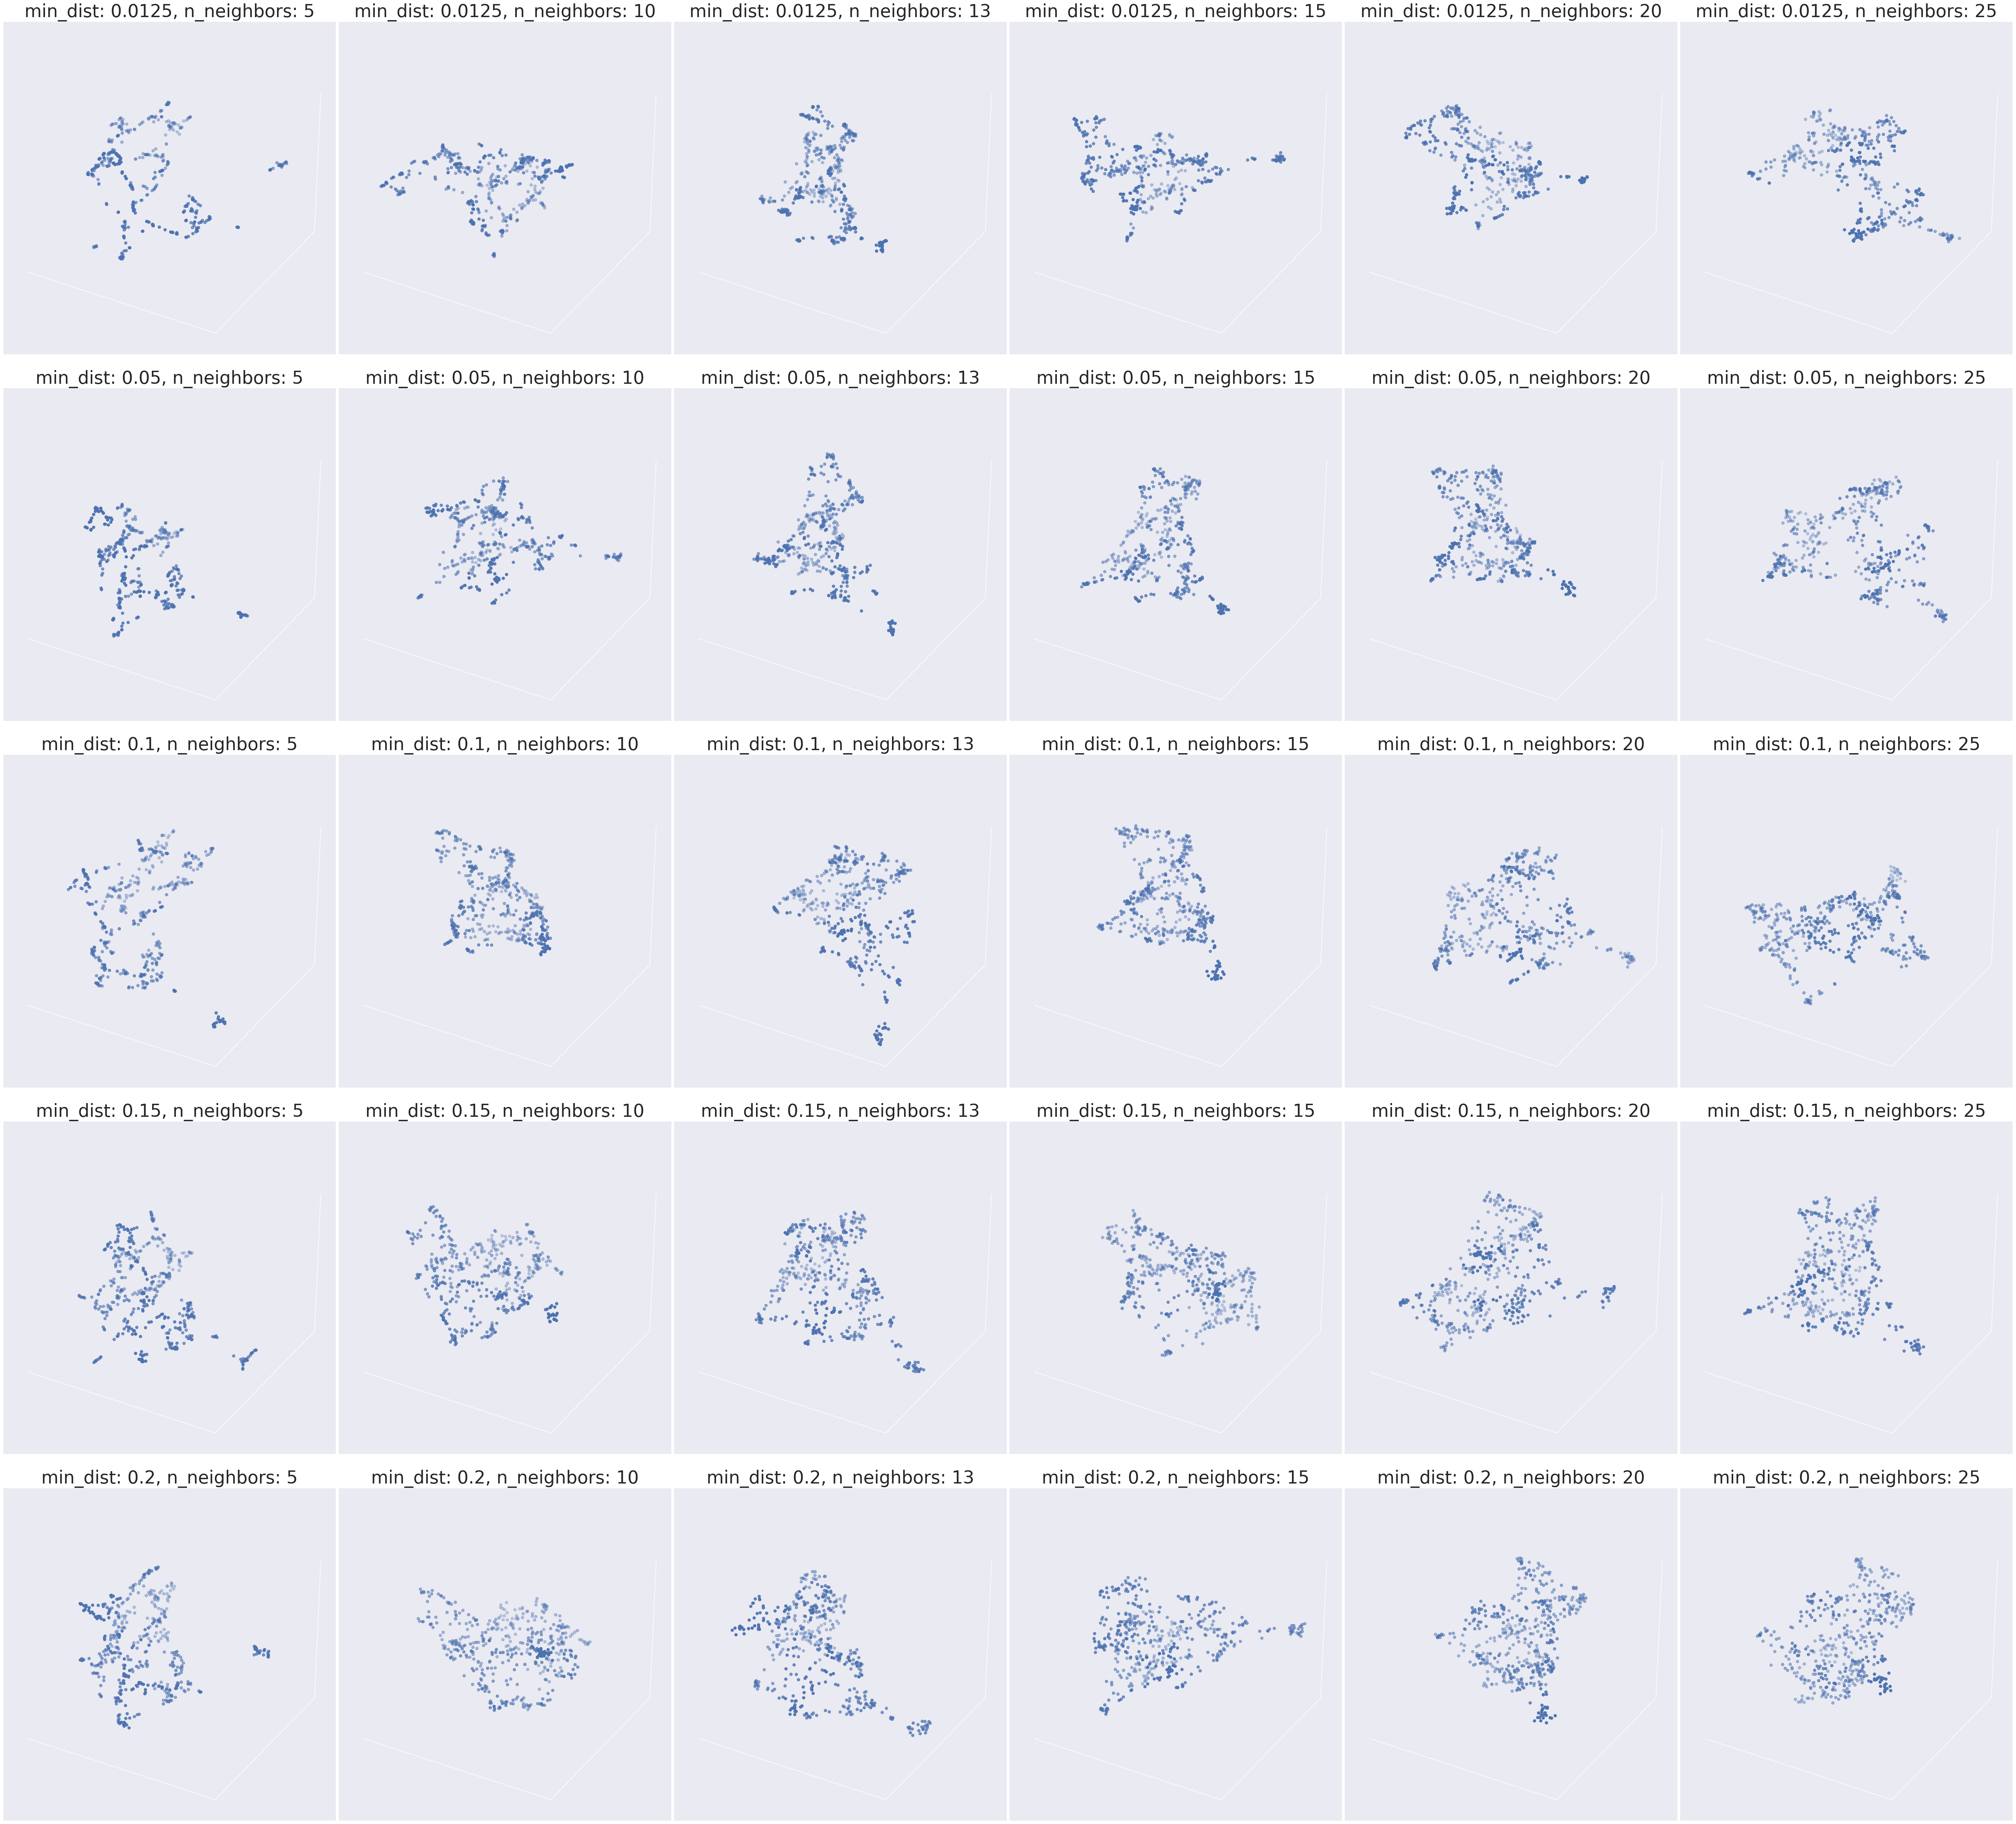
\includegraphics[width=\textwidth]{./images/nomichyp2.png}
    \caption{Nomic, grid search for UMAP hyperparameter (see Table~\ref{tab:umapgrid}) over the parameters \texttt{min\_dist} and \texttt{n\_neighbors}}
    \label{fig:nomic2}
\end{figure}%
\begin{figure}[htbp]
    \centering
    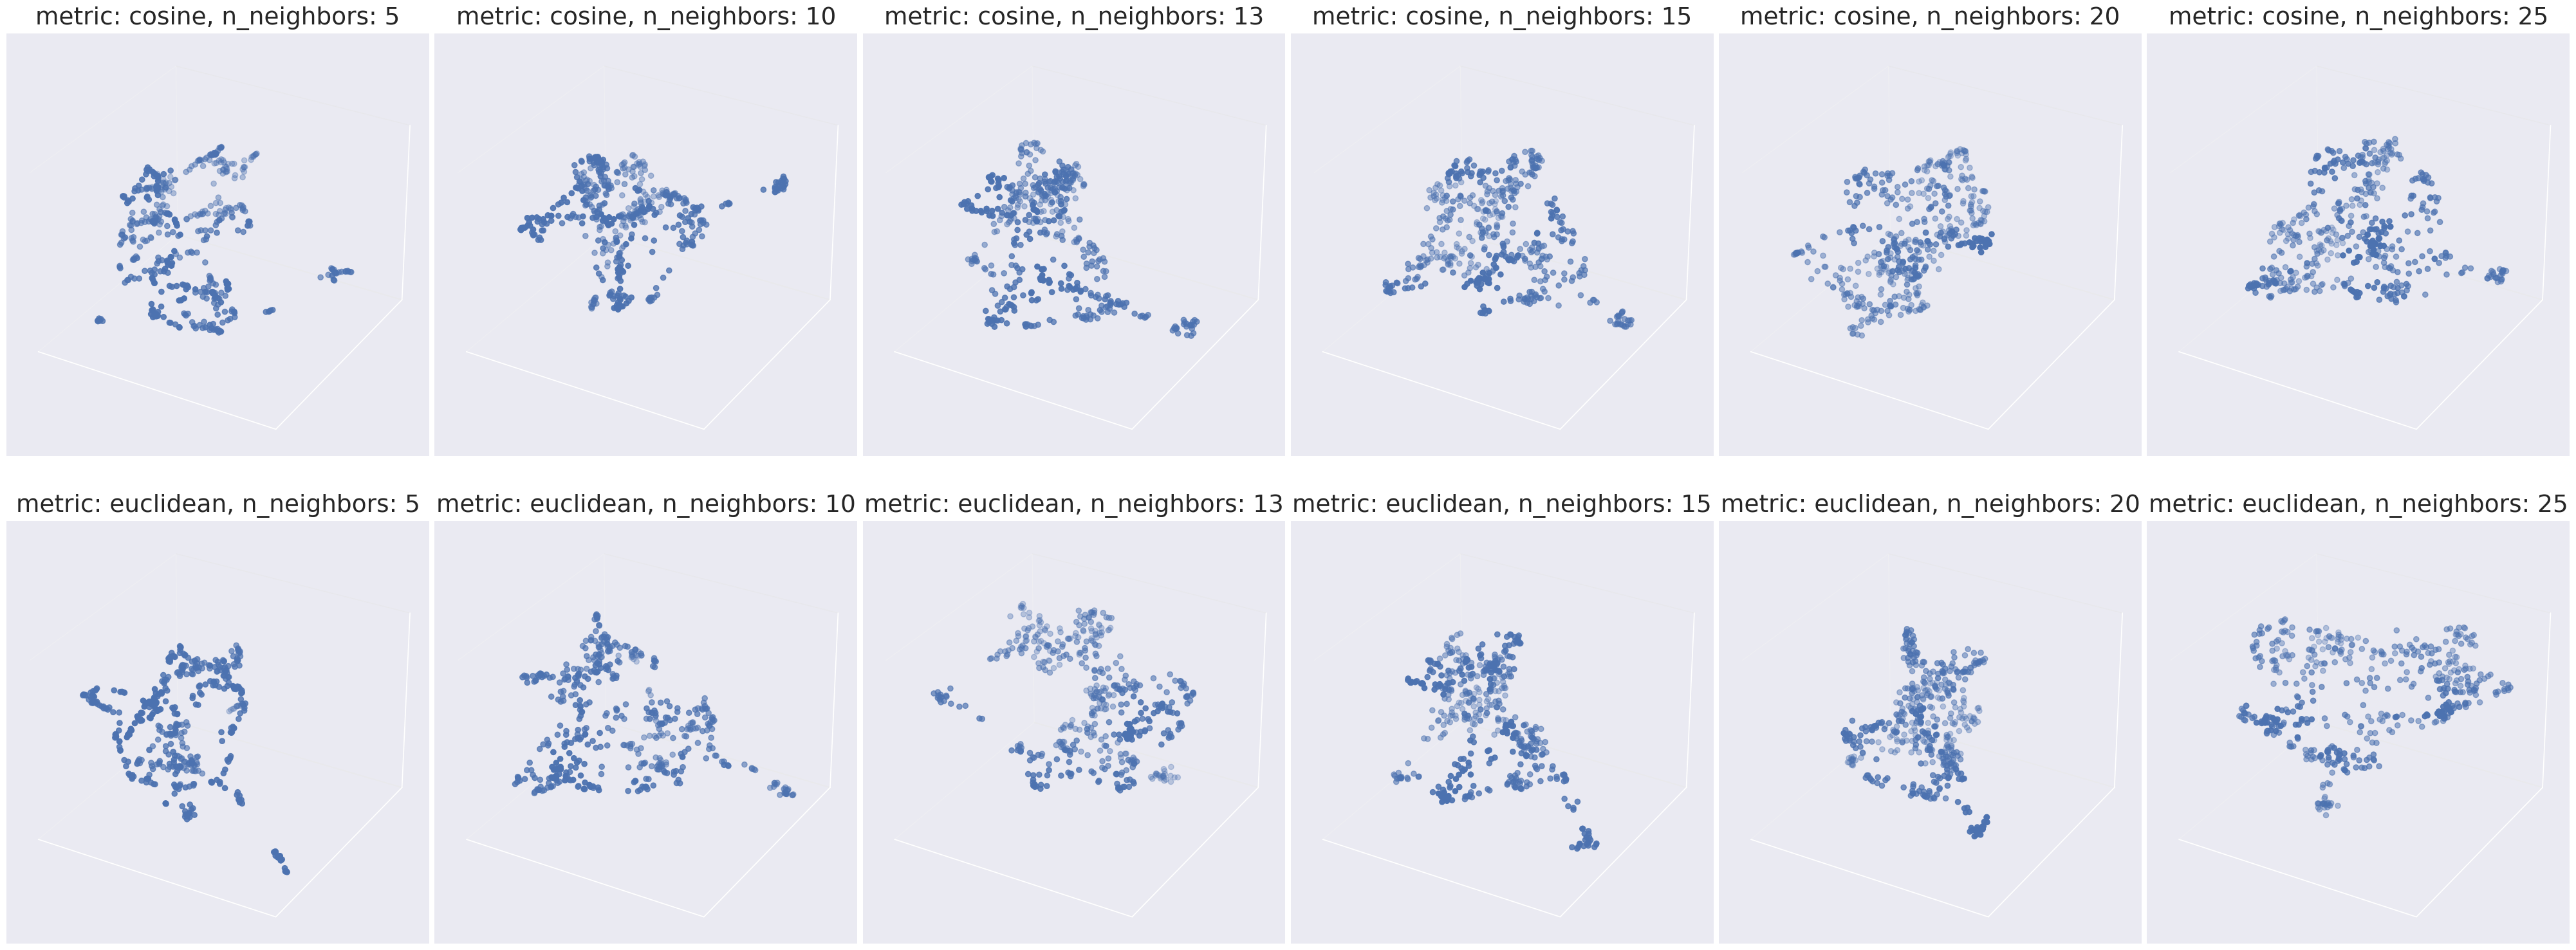
\includegraphics[width=\textwidth]{./images/nomichyp3.png}
    \caption{Nomic, grid search for UMAP hyperparameter (see Table~\ref{tab:umapgrid}) over the parameters \texttt{metric} and \texttt{n\_neighbors}}
    \label{fig:nomic3}
\end{figure}%


\end{document}
